\chapter{Search for H2Mu targeting the VH production mode}\label{chp:VH_analysis}

As described in Section~\ref{sec:hmm_cat_and_strategy}, the analysis in the \VH category targets the \VH production modes of the Higgs boson, 
and is established as two independent parts, the \WH category and the \ZH category.
This chapter provides a full description of the procedures and the results in these two categories.

The \VH analysis focuses on the leptonic ($e$ or $\mu$) decay modes of vector bosons (\PV = \PW or \PZ), 
which lead to distinct final states involving extra well-reconstructed charged lepton(s) in addition to the two muons from the Higgs boson decay.
By requiring these additional leptons, the main backgrounds in the generic $\mu\mu$ phase-space, the \DY and the \ttbar processes, are greatly suppressed,
leading to a high \SoB in the \VH category, and ensuring a good expected significance with only a handful of signal events.
The other decay modes of the vector boson are disregarded for reasons as described below.

The vector bosons decay to tau leptons ($\PW \to \tau+\PGn_{\tau}$, or $\PZ \to \tau\bar{\tau}$) at the same rate as they decay to electrons or muons. 
The reconstruction of $\tau$, as described in Section~\ref{sec:reco_tau}, 
targets the hadronic decays of taus and suffers from a sizable fake rate.
Tagging final states with hadronic tau decays gives a low \SoB phase-space 
and yields negligible contribution to the overall sensitivity.
Tau leptons may also decay into leptons ($e/\mu$ + neutrinos).
The resulting $e$ or $\mu$ only carries about one third of the $\tau$ momentum, 
and has a displacement of a few millimeters from the primary vertex.
The majority of them fail electron or muon selection criteria of the analysis.

The hadronic decays of the \PW or the \PZ boson lead to two jets in the event, making an invariant mass near the mean mass of the boson.
Although amounting to a larger branching ratio than the leptonic decay modes, these hadronic decays turned out not as helpful in enriching the \VH events.
The dijet selection is subject to immense QCD backgrounds and has a much worse mass resolution than for leptons. 
It gives a phase-space dominated by $\ggH+$jets signal vs $\DY+$jets background.
Therefore the hadronic \VH events are considered as minor signal contributions in the \ggH category, 
rather than a dedicated \VH hadronic tag.

The \PZ boson can decay to a pair of neutrinos at a branching ratio of 20\%, 
which leave no electronic signal in the CMS detector and appear as missing transverse momentum (\MET) in the event.
This \MET equals to the \pt of the \PZ boson and can provide discrimination against some backgrounds.
However, as described in Section~\ref{sec:reco_met}, 
the \MET resolution is much worse than those of leptons and jets.
The purity of the $\ZH \to \nu\nu+\mu\mu$ signal can only be enhanced if a very tight cut on the \MET (for example $\MET>100$~\GeV) is applied.
Only a small fraction of \ZH signal would pass this selection 
while some large irreducible backgrounds still remain, like the \ttbar and diboson processes.
Overall, a tag for the $\ZH \to \nu\nu+\mu\mu$ would be much less sensitive than the existing $\ZH \to \ell\ell+\mu\mu$ tag, and is not deployed.
The $\ZH \to \nu\nu+\mu\mu$ signal events are considered as minor signal contributions in the \ggH category.

After requiring additional lepton(s) in the event, the main background in the resulting \VH phase-spaces becomes the \WZ and \ZZ processes, for the \WH and \ZH categories respectively.
For both \WZ and \ZZ backgrounds, if more than two muons are present in the event, 
there are different possibilities of the association between the muons and their parent particles.
In fact, the wrong pairing of muons, called the combinatorial background, yields the majority of the \WZ and \ZZ background.
For example, in an on-shell \WZ event, the muon from the \PW decay can be falsely paired with the oppositely signed (OS) muon from the \PZ decay, 
making an invariant mass near the Higgs boson mass value.
A set of cut-based event selection is optimized to reduced the combinatorial background, further improving the \SoB. 
More details are given in Section~\ref{sec:vh_event_selection}.

The minor backgrounds may include the triboson processes, the \DY process accompanied with additional nonprompt leptons, 
or the \Pqt quark associated processes, for example the \ttbar, $\Pqt\PW$, and $\ttbar\PV$ processes, 
where the \Pqb quarks from the top decays either fall out of the acceptance of the detector or fails the b-tagging. 
All these minor backgrounds have different kinematic profiles from the signal and can be reduced to different extents. 
Multivariate discriminators are trained in both the \WH and the \ZH categories to account for the differences between the signal and the inclusive background as much as possible.

Events are further divided in to several subcategories with different \SoB based on the Multivariate discriminators. 
In each subcategory, the \mmm spectrum is plotted, and analytic functions are used to model the shapes of signal and background.
The strength of the \hmm signal is evaluated by fitting the signal and the background functions to the \mmm spectrum of data.

The following sections of this chapter are organized as follows: 
Section~\ref{sec:vh_event_selection} describes the event selection. 
Section~\ref{sec:vh_bdt_cats} discusses the details of the training of the MVA discriminators, and the determination of subcategories based on them.
Section~\ref{sec:vh_sig_bkg_model} shows the performances of different analytic functions on the signal and background modeling.
Section~\ref{sec:vh_systematics} lists different sources of systematic uncertainties considered in this analysis.
And Section~\ref{sec:vh_results} gives the statistical interpretation of the results.


\section{Event selection}\label{sec:vh_event_selection}
The \VH analysis takes standard CMS physics objects described in Chapter~\ref{chp:objects},
whose selections in this analysis are detailed in Section~\ref{sec:obj_sel}.
The selection criteria for electrons and muons, which are the most important for this analysis, are also summarized in Table~\ref{tab:vh_lep_sel}.

\begin{table*}[!htb]
    \centering
    \captionsetup{justification=centering}
    \topcaption{Selection criteria on muons and electrons in the VH analysis.}
    \begin{tabular}{lcc}
    \hline
    Variable               & Muon                      & Electron \\
    \hline
    \pt                    & $>$ 20\GeV                & $>$ 20\GeV       \\
    $|\eta|$               & $<$ 2.4                   & $<$ 2.5          \\
    ID and Iso             & Medium ID + Loose Iso     & MVA wp90         \\
    ECal gap veto          & -                         & $(1.444,1.566)$  \\
    $d_{xy}$(PV)           & $<$ 0.05 cm               & $<$ 0.05 cm      \\
    $d_{z}$(PV)            & $<$ 0.10 cm               & $<$ 0.10 cm      \\
    SIP                    & $<$ 8.0                   & $<$ 8.0          \\
    Conversion Veto        & -                         & \checkmark       \\
    Number of Missing Hits & -                         & $<$ 2            \\
    lepMVA                 & $>$ 0.4                   & $>$ 0.4          \\
    \hline
    \end{tabular}
    \label{tab:vh_lep_sel}
\end{table*}

The event selection targets the leptonic decays of the \PW or the \PZ bosons in the \VH signals.
The selection steps are devised to suppress different background processes 
and optimize the \SoB in the \WH and \ZH categories respectively. 
The event selection in the $\WH \to \ell\nu+\mu\mu$ category is described as follows:
\begin{itemize}
	\item At least one muon must have \pt $>$ 26\GeV /29\GeV /26\GeV 
	      for years 2016/2017/2018 respectively, which is matched to a
              single-muon trigger object
	\item All SFOS lepton pairs must have an invariant mass $> 12$~\GeV
	\item The charge of the three leptons must add up to $\pm 1$
	\item At least one $\mu^{+}\mu^{-}$ pair must have an invariant mass between 110
	      and 150~GeV
	\item If two $\mu^{+}\mu^{-}$ pairs fall in the 110 - 150~GeV mass window, the pair
	      with the higher \pt is chosen as the Higgs candidate (denoted $\mu\mu_{\PH}$)
	\item The event must contain exactly 0 medium b-tagged jet and less than 2 loose b-tagged jets
	\item In 3$\mu$ events, the non-Higgs-candidate $\mu^{+}\mu^{-}$ pair ($\mu\mu_{OS}$) must
	      not have an invariant mass between 81 and 101~\GeV, to suppress WZ and Z+jets backgrounds
\end{itemize}
The event selection in the $\ZH \to \ell\ell + \mu\mu$ category is described as follows:
\begin{itemize}
	\item At least one muon must have \pt $>$ 26\GeV /29\GeV /26\GeV 
	      for years 2016/2017/2018 respectively, and the event must
	      contain an unprescaled single-muon trigger object
	\item The charge of the four leptons must add up to 0.
	\item All SFOS lepton pairs must have an invariant mass $> 12$~\GeV.
	\item In $\mu\mu ee$ events, the $e^{+}e^{-}$ pair must have invariant mass between 70 and 110 GeV, and the $\mu^{+}\mu^{-}$ pair must have invariant mass between 110 and 150 GeV.
	\item In 4$\mu$ events, if it is possible to form two distinct $\mu^{+}\mu^{-}$ pairs
          each with a mass between 81 and 101~GeV, the event is discarded.
	\item In 4$\mu$ events, one muon pair must have mass between 110 and 150 GeV, and the other muon pair must have mass between 81 and 101 GeV.
	\item In 4$\mu$ events, if both combinations have a muon pair in the Z-mass window and a muon pair in the signal-mass window, the combination in which the mass of the Z candidate is closer to 91 GeV is chosen. 
	\item The event must contain exactly 0 medium b-tagged jet and less than 2 loose b-tagged jets.    
\end{itemize}
These selection criteria are also summarized in Table~\ref{tab:vh_evt_sel}.
\begin{table*}[!htb]
    \centering
    \captionsetup{justification=centering}
    \topcaption{Event selections for the \WH and \ZH categories.}
    \resizebox{\textwidth}{!}{\begin{tabular}{lcc}
    \hline
    Criterion                                                & \WH category            & \ZH category\\
    \hline
    Muon trig match                                          & \checkmark              & \checkmark \\
    b-jets veto, 0 medium and $<$ 2 loose                    & \checkmark              & \checkmark \\
    $\mu^{+}\mu^{-}$ pair with $110<\mmm<150~\GeV$           & \checkmark              & \checkmark \\
    Additional lepton(s)                                     & 1                       & 1 SFOS pair \\
    Low-mass resonance veto $m_{\ell\ell}>12~\GeV$           & \checkmark              & \checkmark \\
    Number of $|\mmm-m_{\PZ}|<10~\GeV$ or $|m_{\Pe\Pe}-m_{\PZ}|<20~\GeV$     & $=$ 0          & $=$ 1  \\
    Choice of muon combination                               & Highest $p_T(\mu\mu)$ as $\mu\mu_{\PH}$  & Smallest $|\mmm-m_{\PZ}|$ as $\mu\mu_{\PZ}$ \\
    \hline
    \end{tabular}}
    \label{tab:vh_evt_sel}
\end{table*}

%\textcolor{red}{efficiency of sig combo and bkg combo,
%plots before and after.}


\section{MVA discrimination}\label{sec:vh_bdt_cats}

After the event selection of the \WH or the \ZH categories, the remaining background processes 
resemble the kinematic signatures of the signals and cannot be decisively reduced by simple selection cuts.
MVA discriminators are trained to further enhance the \SoB.
The algorithm used in this analysis is called the Boosted decision tree (BDT),
which is a supervised machine learning algorithm that classifies data by 
iteratively generating and averaging (boosting) a series of decision trees.

Different variables can be effective in separating different background processes.
For example, the muon pair from \Pqt quark associated processes usually have more \pt than those from the \WH signal process,
while the \MET in the \DY process is likely to be smaller than that in the \WH events.
The main background, \WZ or \ZZ in the \WH and \ZH categories respectively, 
in which the Higgs candidate $\mu\mu$ pair comes from an off-shell \PZ boson,
is a more complicated story as it looks almost kinematically identical to the signal.  
The key in discriminating them lies in the spin difference between the \PZ and the \PH bosons,
which is measured as a difference in the helicity angle $\theta^{*}$ between the decay products of the \PZ (\PH) boson.

The helicity angle is defined in a decay system in the frame in which the parent particle is at rest,
as the angle between the direction of the decay and the boost direction of the parent particle.
The distribution of this angle is determined by the spins of the parent particle and the decay products.
In the case of $\PW \to \WZ$ ($\PZ \to \ZZ$) vs $\PW \to \WH$ ($\PZ \to \ZH$), the helicity angle between the \PW ($\PZ_{1}$) and the $\PZ_{2}$ follows the distribution $1 + cos^{2}\theta^{*}$ %\textcolor{red}{a illustrative figure},
while the the helicity angle between the \PW (\PZ) and the \PH follows a flat distribution.
Similarly, for \zmm vs \hmm, the muons from a \PZ decay tend to align with the polarization of the \PZ boson, 
while the muons from a \PH decay do not have a preference in direction.

All these helicity angles, $\theta^{*}_{\WH}$, $\theta^{*}_{\ZH}$, and $\theta^{*}_{\mu\mu}$, 
can in principle provide significant discrimination between the signal and the background.
However, in practice, $\theta^{*}_{\WH}$ cannot be reconstructed because of the lack of information of the neutrino from the \PW decay, 
and the distribution of $\theta^{*}_{\mu\mu}$ is severely sculpted by the acceptance of the CMS detector, 
rendering a similar shape for the \zmm and \hmm processes.
On the other hand, the spin information can be partially captured in other variables, 
for example the helicity angle between the \PW-lepton and the $\mu\mu_{\PH}$ system, 
and some other angular correlations like $\Delta\phi$, $\Delta\eta$.
All these variables are tested as inputs to the BDT for the performance.
Some of them turned out insignificant and are later trimmed off from the input collection.
To make sure the BDTs do not sculpt the \mmm shape, which will be used for the signal extraction,
variables that are strongly correlated with \mmm, for example the \pt of the muons, are not used in the BDTs.  


\subsection{BDT targeting \texorpdfstring{$\WH \to \ell\nu+\mu\mu$}{WH to 3l} signal}\label{subsec:WHlep_BDT}

The \WH BDT takes variables of three different kinds, the kinematic variables of leptons that are uncorrelated with \mmm,
the angular correlations between different leptons as discussed above, and the variables reflecting the missing energy in the event.
In total, there are 16 input variables to the BDT, which are listed in Table~\ref{tab:wh_bdt_vars}. 
The variables related to the missing energy includes the missing energy itself, 
the transverse mass (\MT) between a lepton and the missing energy, and the angular separation between a lepton and the missing energy.
Two types of missing energy are tested, \MET, which is the negative of the vector sum of the \pt of all PF candidates, 
and \MHT, which only considers well-defined jets, photons, and leptons in the similar calculation.
The \MET-related and \MHT-related variables are expected to play interchangeable roles in the BDT.
The \MHT-related variables turned out to be slightly better performing and are kept in the final BDT,
while the \MET-related variables are trimmed.

Another important feature in the \WH category is that about 40\% of the \WZ background are from the wrong combination of muons in 3$\mu$ events.  
The duplication of some variables calculated with the alternative combination of the muons in each event may also help with the discrimination.
For example, apart from the transverse mass between the nominal \PW-lepton and the the \MHT, 
another transverse mass is also considered, using the \MHT and the same-sign muon from the nominal Higgs candidate,
which turns out to be effective.

\begin{table*}[!htb]
  \centering
  \captionsetup{justification=justified}
  \topcaption{List of input variables used to train the signal-background
           separation BDT in the WH category. In this table, $\mu\mu_{\PH}$ is the Higgs candidate, 
           $\ell$ is the lepton from the W decay, $\mu_{OS}$ ($\mu_{SS}$) refers to the muons in the Higgs candidate which OS (SS) to the lepton.}
  \begin{tabular}{lc}
  \hline
   Variable                            &  Description  \\
  \hline
   $\pt(\mu\mu_{\PH})$                 & \pt of the Higgs candidate \\
   $|\eta(\mu_{1})|$                   & $\eta$ of the leading muon in the Higgs candidate \\
   $|\eta(\mu_{2})|$                   & $\eta$ of the trailing muon in the Higgs candidate \\
   $\Delta$R($\mu_{SS}, \mu_{OS}$)     & $\Delta$R between the two muons in the Higgs candidate \\
   \pt($\ell$)                         & \pt of the extra lepton in the event \\
   Number of electrons                 & Number of electrons in the event  \\
   $\Delta$R($\ell, \mu\mu_{\PH}$)     & $\Delta$R between the extra lepton and the Higgs candidate \\
   $\Delta\eta$($\ell, \mu\mu_{\PH}$)  & $\Delta\eta$ between the extra lepton and the Higgs candidate  \\
   $\Delta\eta$($\ell, \mu_{SS}$)      & $\Delta\eta$ between the extra lepton and the SS muon \\
   $\cos\theta^*(\ell, \mu_{SS})$      & $\cos\theta^*$ between the extra lepton and the SS muon \\
   $\Delta$R($\ell, \mu_{OS}$)         & $\Delta$R between the extra lepton and the OS muon \\
   $\Delta\eta$($\ell, \mu_{OS}$)      & $\Delta\eta$ between the extra lepton and the OS muon  \\
   $\cos\theta^*(\ell, \mu_{OS})$      & $\cos\theta^*$ between the extra lepton and the OS muon \\
   $\MT(\mu_{SS}, $MHT$)$              & transverse mass of the \MHT and the SS muon \\
   $\MT(\ell, $MHT$)$                  & transverse mass of the \MHT and the extra lepton \\
   $|\Delta\phi(\ell, $MHT$)|$         & $|\Delta\phi|$ between the \MHT and the extra lepton \\
  \hline
  \end{tabular}
  \label{tab:wh_bdt_vars}
\end{table*}

The sensitivity of this analysis depends largely on the resolution of the \mmm peak, which is determined by muon momentum resolution
and in turn primarily depends on $\eta$ of the muons as the detector condition differs in different $\eta$ regions in CMS.
It is important to divide events with different resolution into different categories, which leads to an enhancement to the overall \SoB.
In the previous \hmm analysis~\cite{PhysRevLett.122.021801, carnesthesis}, the categorization is achieved by dividing events based on 
both the BDT output and the $\eta$ value of the muons.  
While in this work, the resolution information is incorporated into the BDT, not as an input variable, but by weighting the signal events by 1/$\sigma(\mmm)$,
which is the per-event experimental dimuon mass resolution, calculated from the \pt uncertainty of the muon tracks.
In this way, the BDT output encapsulates both the kinematic information and the resolution information in its output, 
allowing for a categorization based on a single variable, achieving a better significance with fewer categories.
The resolution is not used as an direct input to the BDT because its distribution is not very different between signal and background.
The weights are only applied in the training on signal events, and not applied in the evaluation of the BDT score.

The BDT is trained with a collection of simulated samples from all eras in Run 2.  
The training is performed in the mass window of $110 ~\GeV{} < \mmm < 150 ~\GeV{}$.  
To make sure the BDT is not sensitive to the \mmm value, signal samples with different Higgs boson mass assumptions, 
$\mh = 120, 125, 130$ GeV, are all used as signals in the training.  
Signal events are only used if the candidate $\mu\mu$ pair truly originates from the Higgs boson decay, 
so that the BDT only picks the true kinematic signatures of the signal. No parent matching is required for backgrounds.   
To benefit from the maximal statistics in simulation while keeping sensitive to all kinematic features, 
events with $e+\mu\mu$ and $\mu+\mu\mu$ are used together in the training, but can be distinguished 
by the "number of electrons" as one of the input variables to the BDT.  
To increase the statistics of the nonprompt backgrounds in the simulated events, 
a relaxed lepMVA cut is used for the training collection than in the actual analysis, 
and the nonprompt yields are scaled by a factor of 0.5 to account for the increased nonprompt lepton efficiency.  
For both the signal and background samples, half of the events is used for the training, 
while the other half is used for the testing.

A receiver operating characteristic (ROC) curve illustrates the performance of binary classifiers 
by plotting the true positive rate against the false positive rate.
The BDT output and its ROC curve are shown in Figure~\ref{fig:wh_bdt_output}, 
in which the BDT performs the same on training and testing samples, indicating no over-training.
Distributions of the BDT input variables are shown in Figures~\ref{fig:wh_bdt_vars}.


\begin{figure}[!htb]
      \centering
      \captionsetup{justification=justified}
      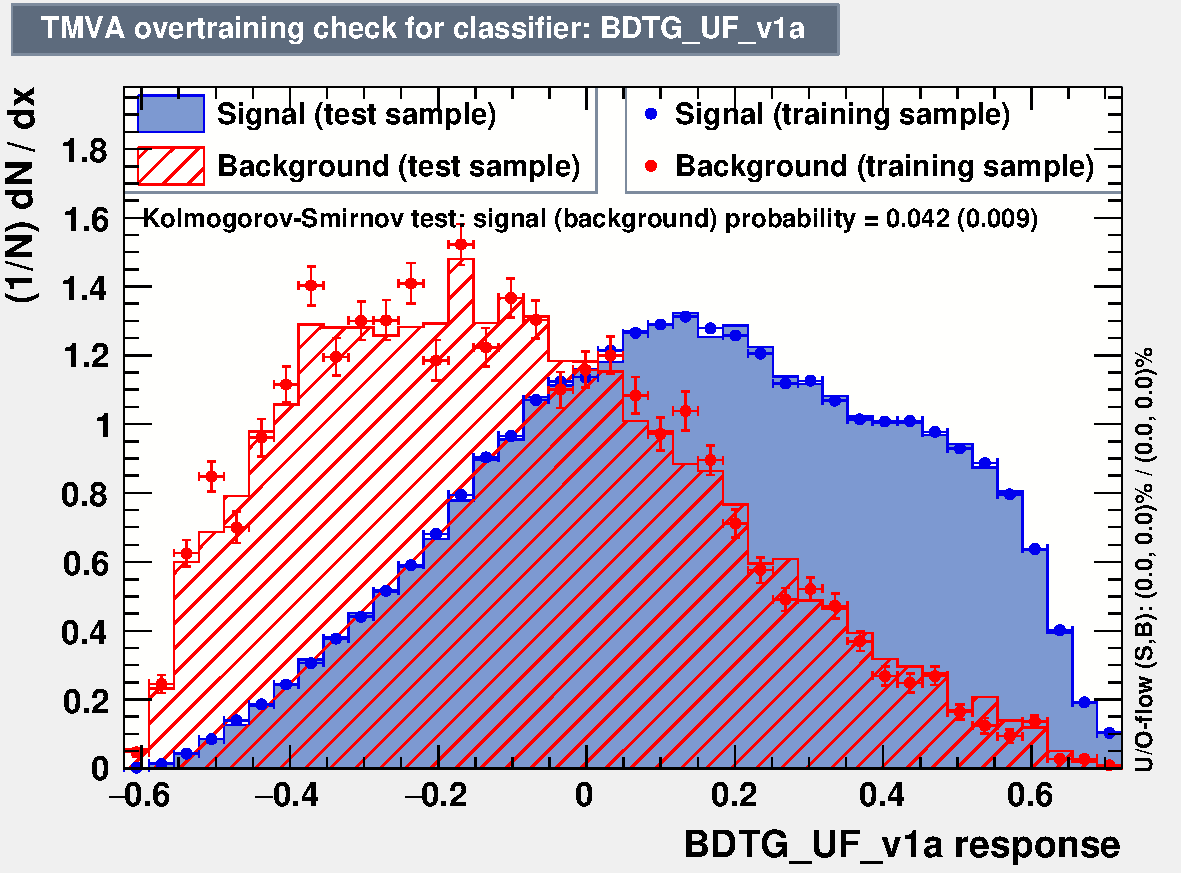
\includegraphics[width=0.50\textwidth]{pics/VH_sec/BDT_train_WH/WH_BDT_overtrain.pdf}
      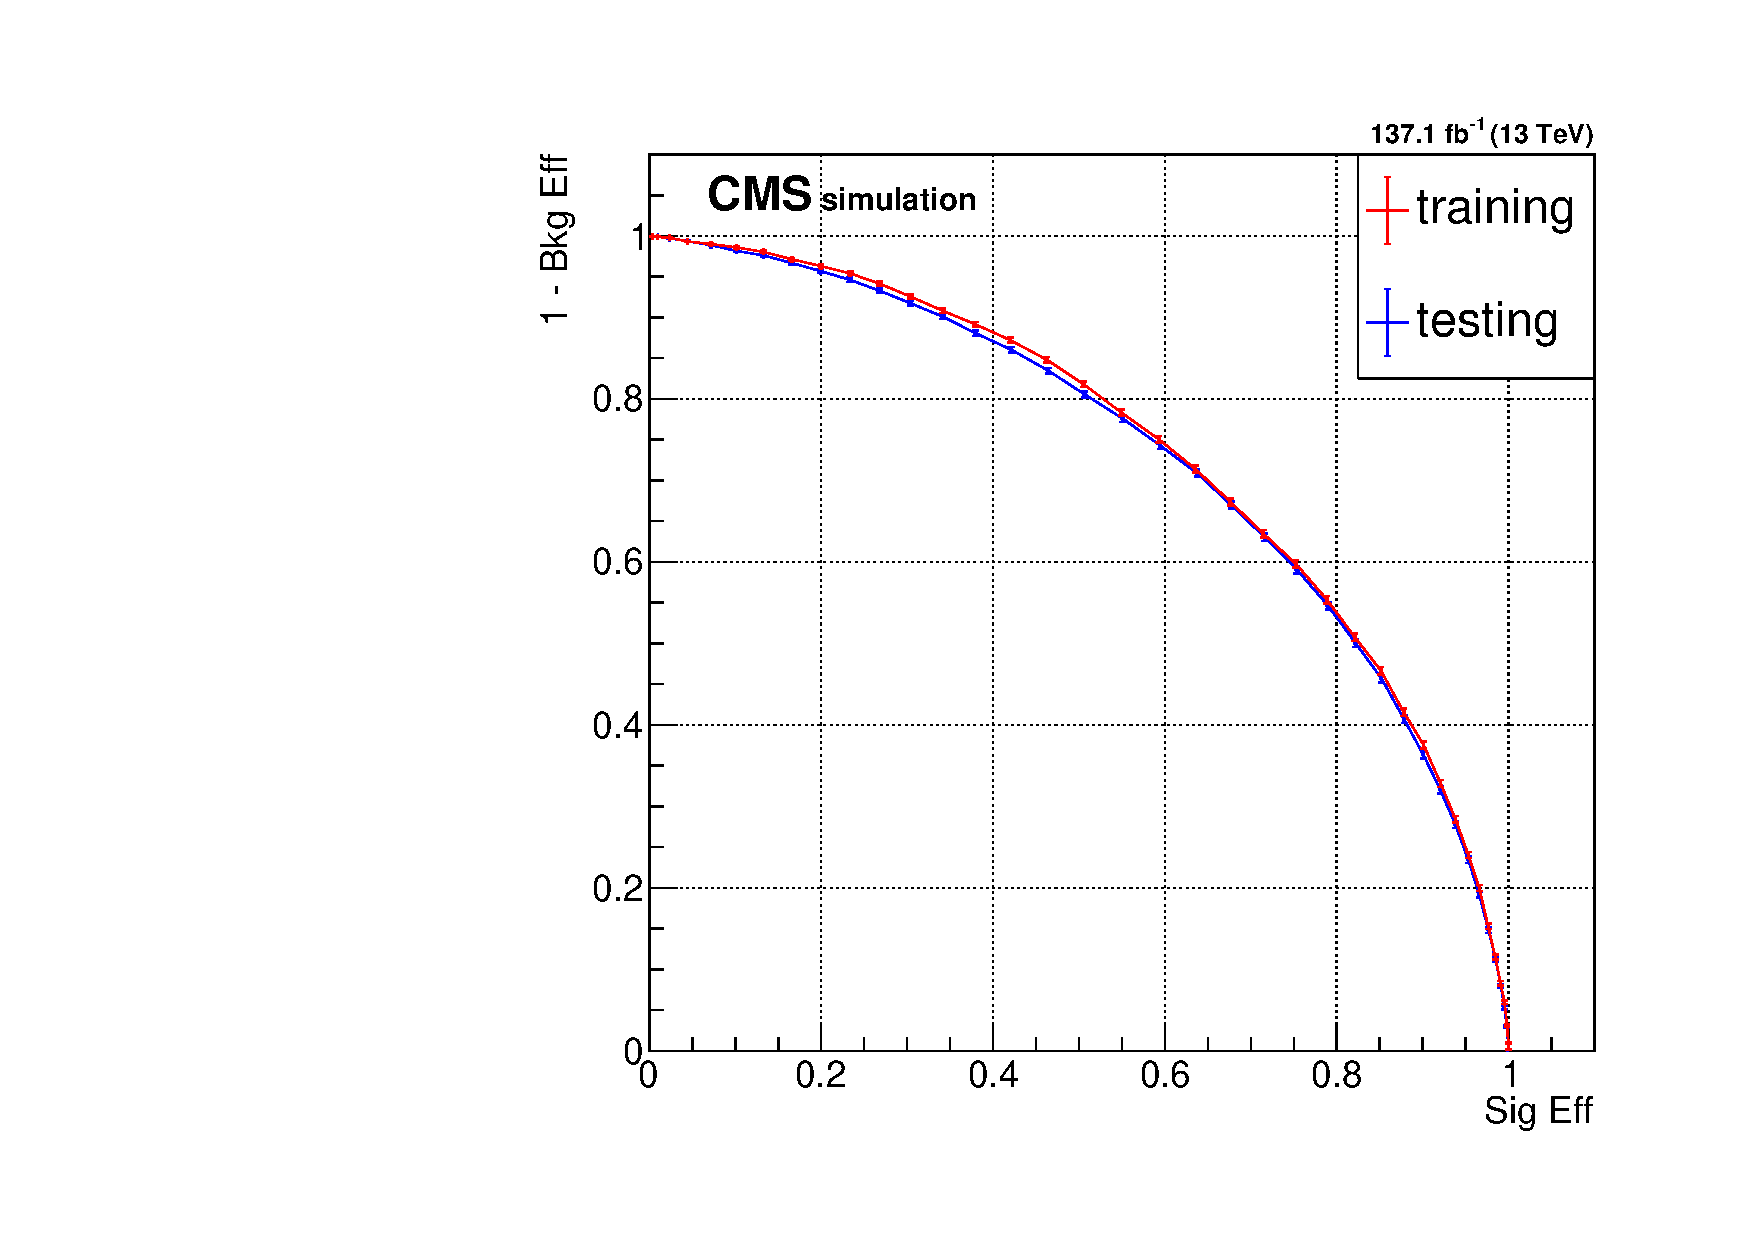
\includegraphics[width=0.43\textwidth]{pics/VH_sec/BDT_train_WH/WH_BDT_ROC.pdf}
      \caption{Plots of the performance of the \WH $\to 3\ell$. 
               On the left, the BDT output score, with signal in blue and background in red.  
               On the right, the receiver operating characteristic (ROC) curve, 
               with training sample in red and testing sample in blue. 
               A slight over-training is observed in the region of low signal efficiency, because of the fluctuation in background. 
               As will be shown in Fig.~\ref{fig:wh_bdt_mass}, the BDT dose not sculpt the shape of $\mmm$.}
      \label{fig:wh_bdt_output}
  \end{figure}
  
  \begin{figure*}[!htb]
      \centering
      \captionsetup{justification=justified}
      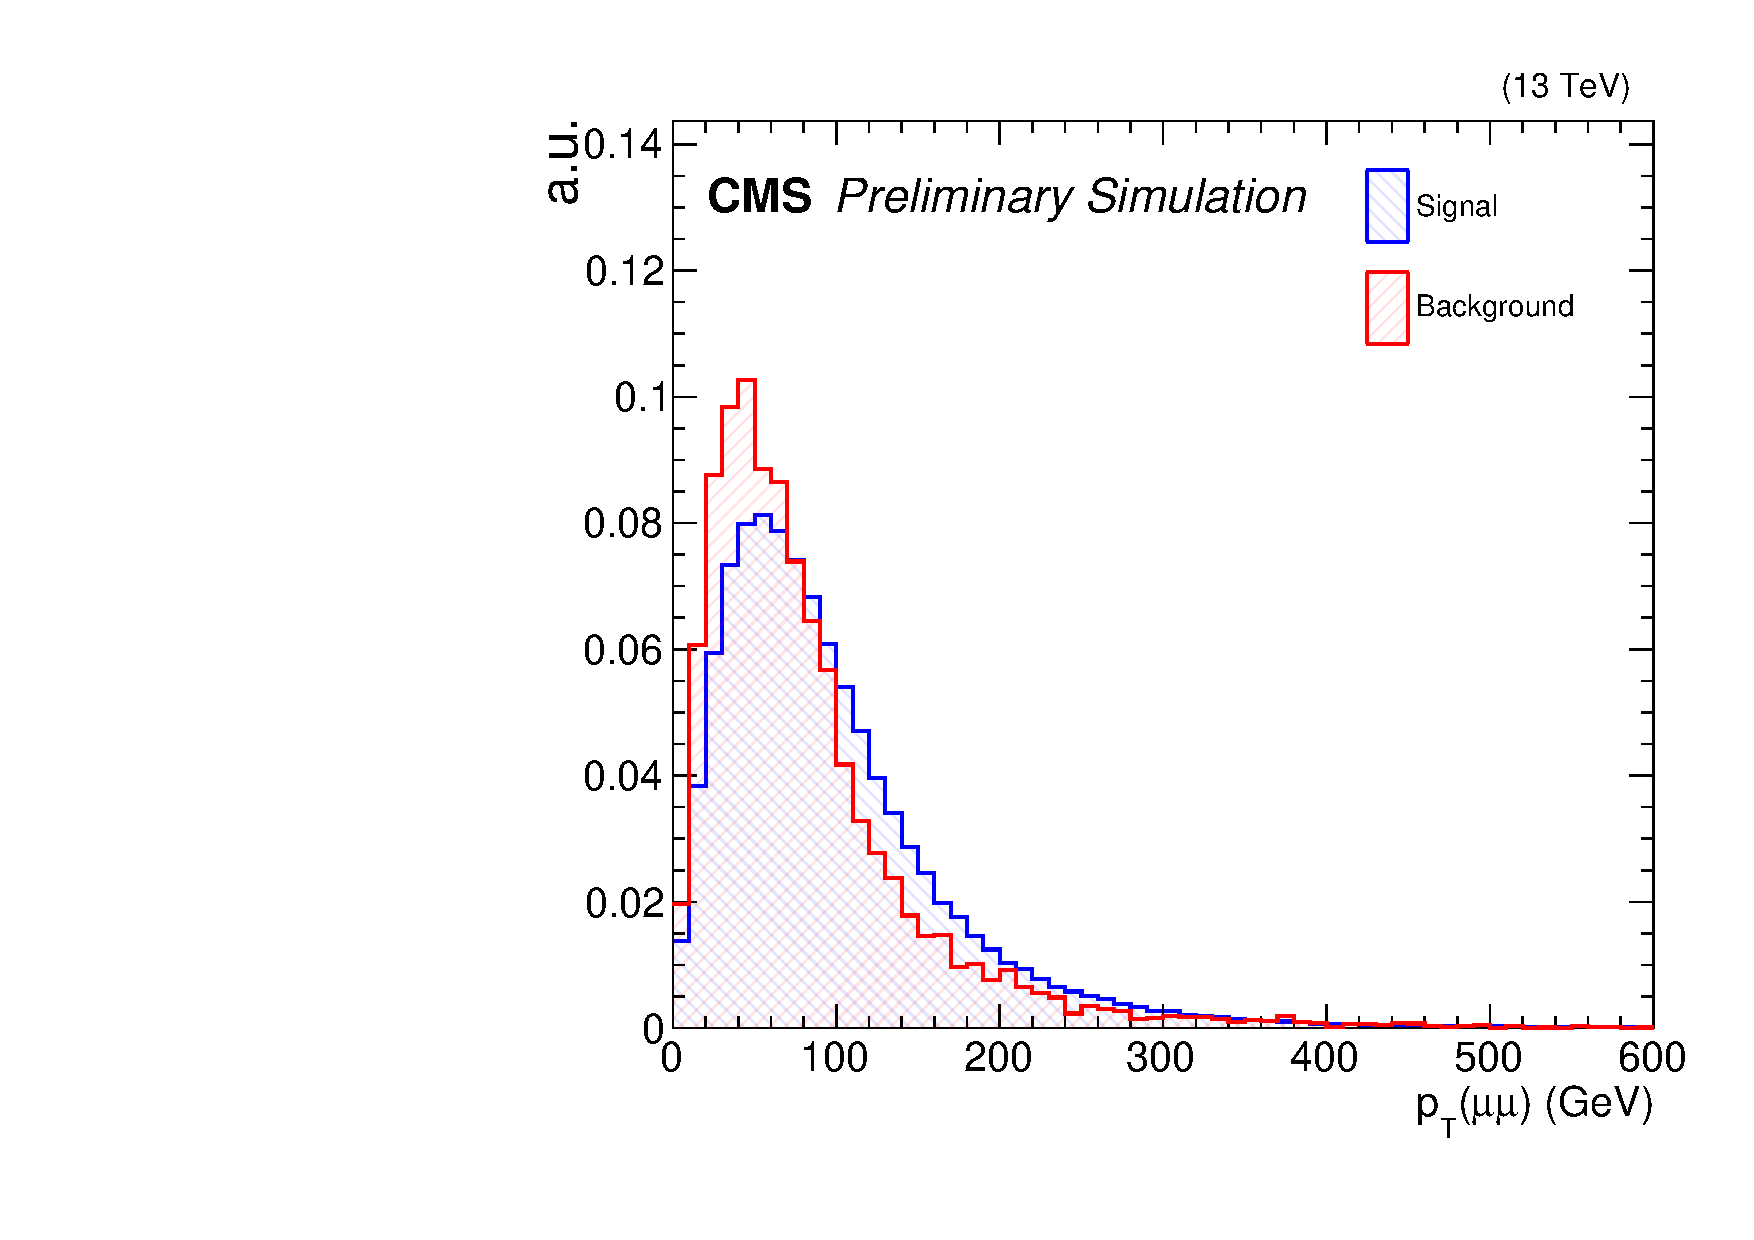
\includegraphics[width=0.24\textwidth]{pics/VH_sec/BDT_train_WH/BDT_H_pair_pt.pdf}
      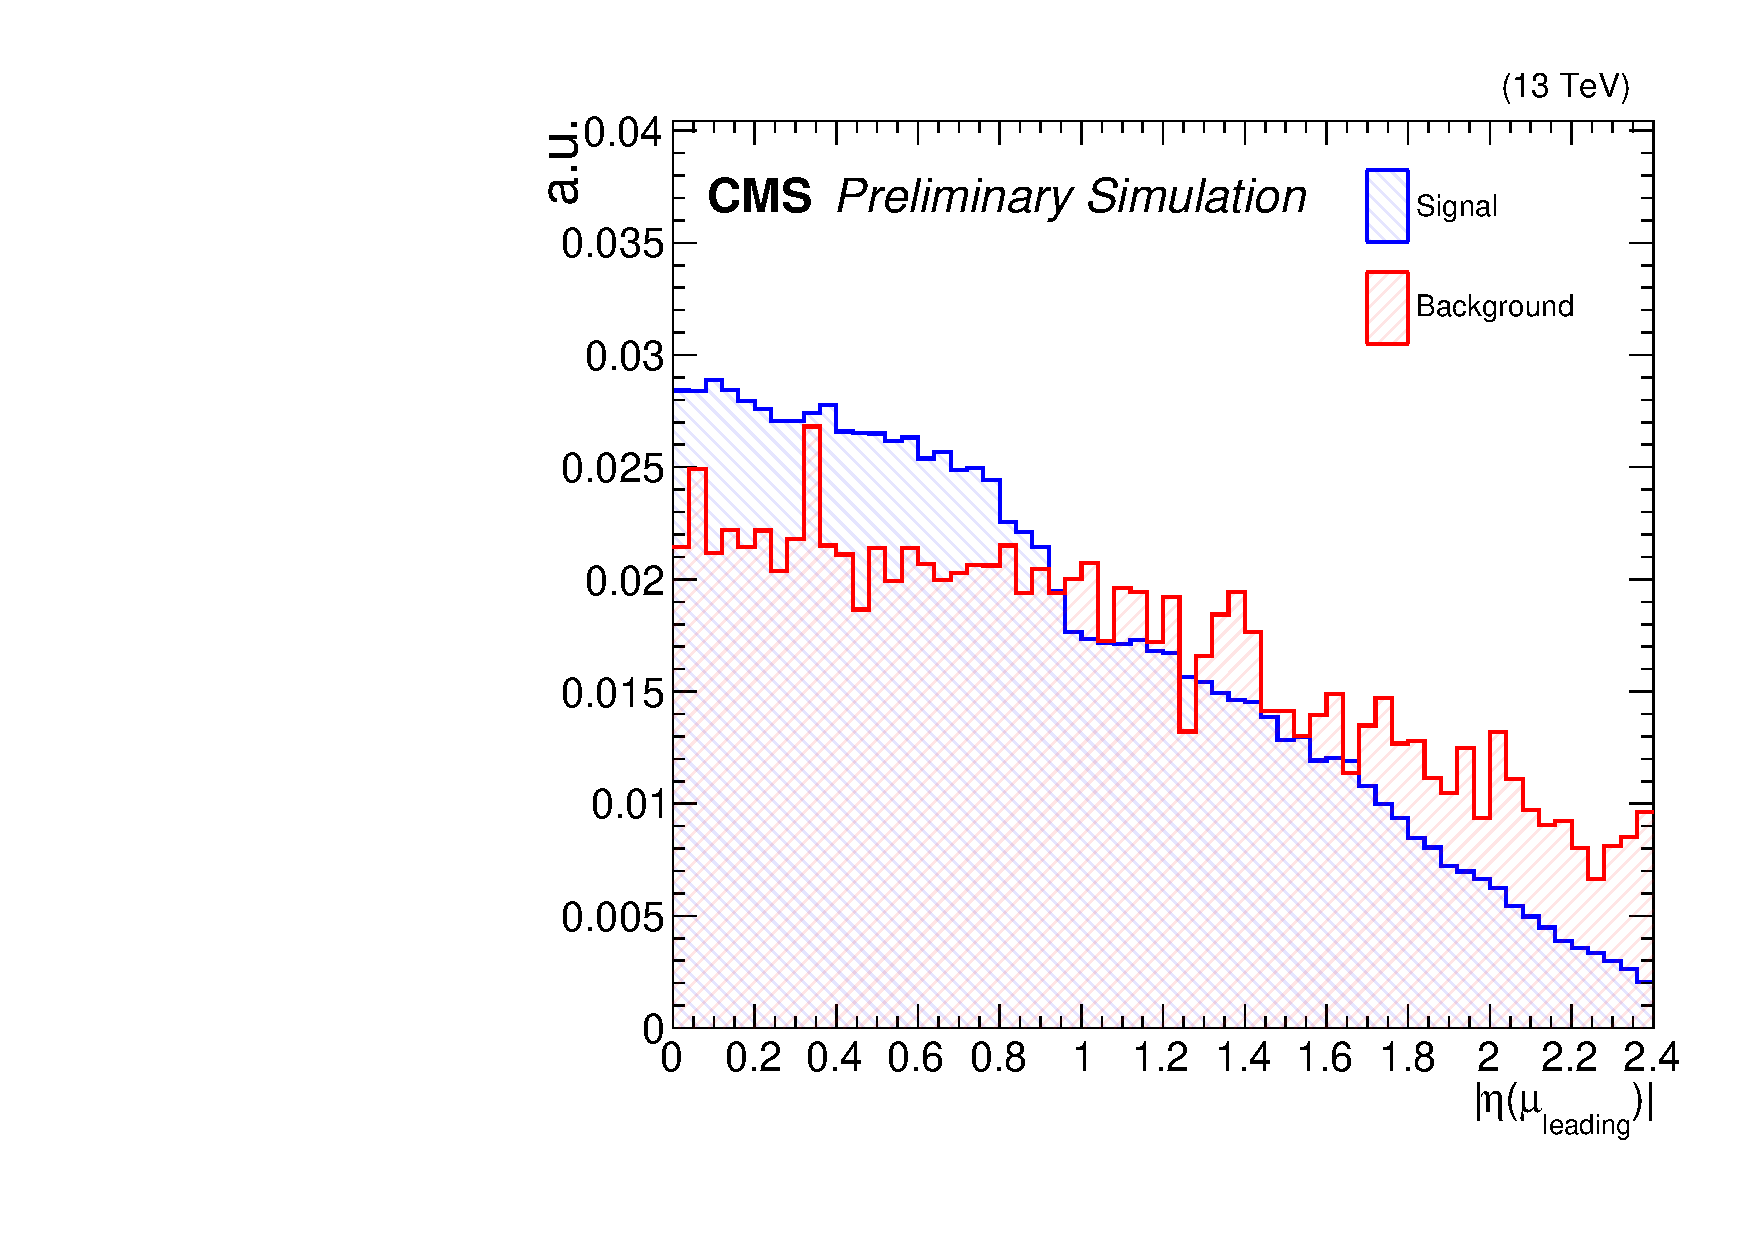
\includegraphics[width=0.24\textwidth]{pics/VH_sec/BDT_train_WH/BDT_muH1_eta_abs.pdf}
      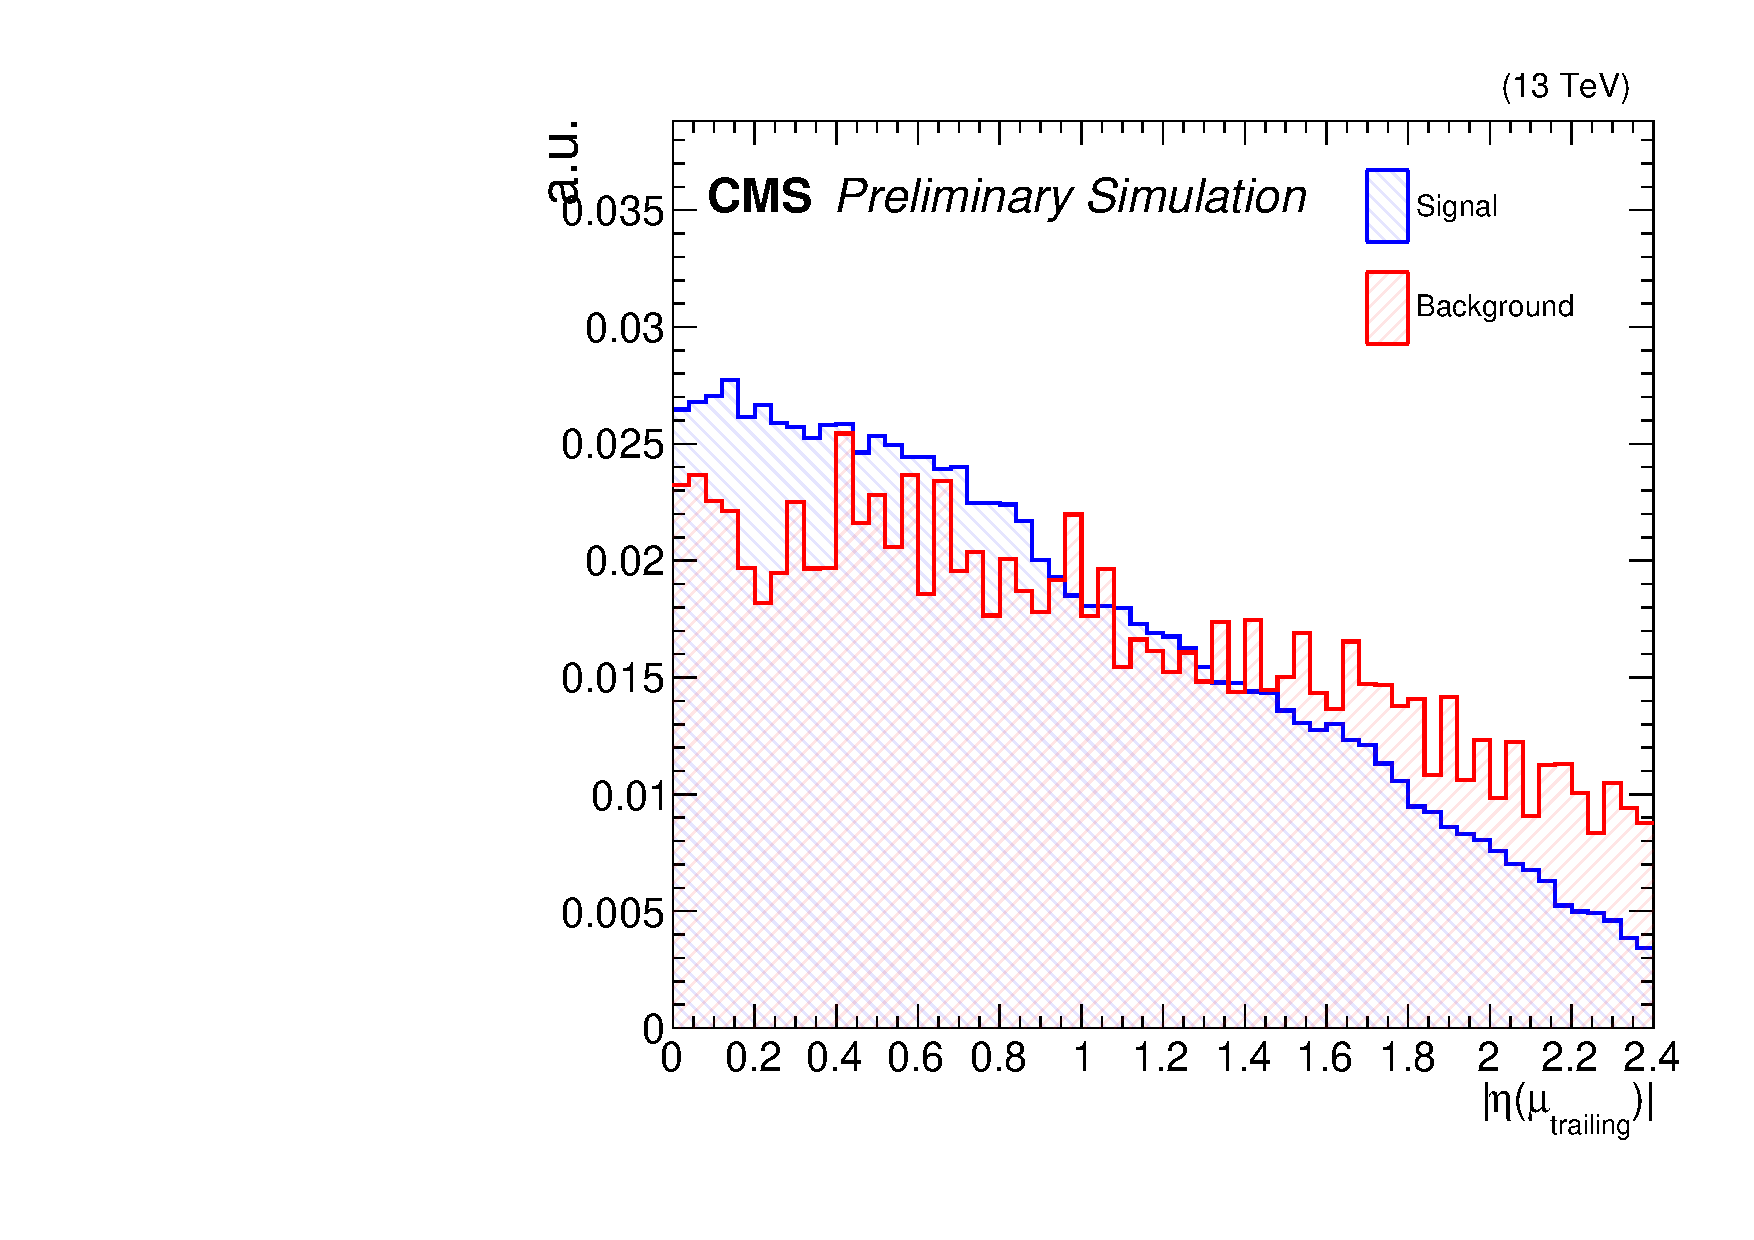
\includegraphics[width=0.24\textwidth]{pics/VH_sec/BDT_train_WH/BDT_muH2_eta_abs.pdf}
      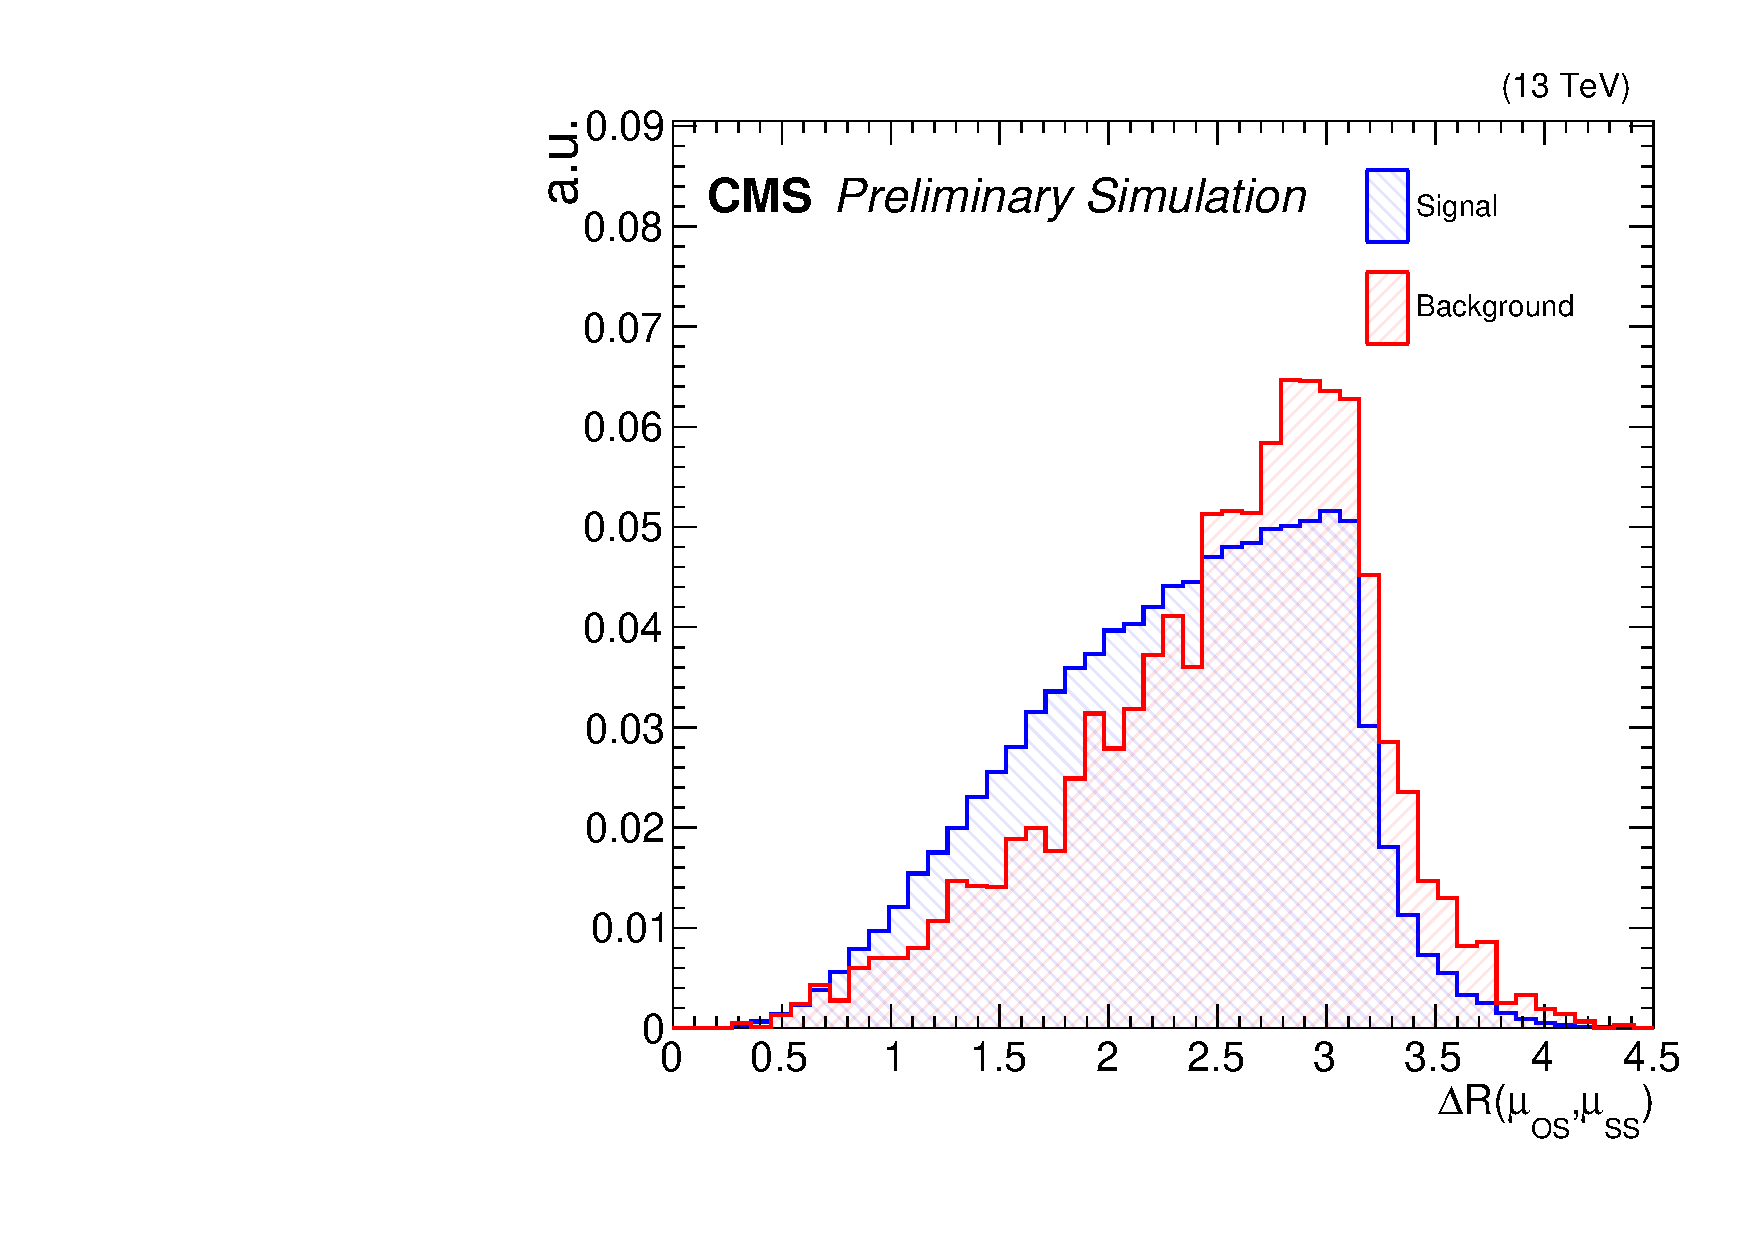
\includegraphics[width=0.24\textwidth]{pics/VH_sec/BDT_train_WH/BDT_muSS_muOS_dR.pdf}
  
      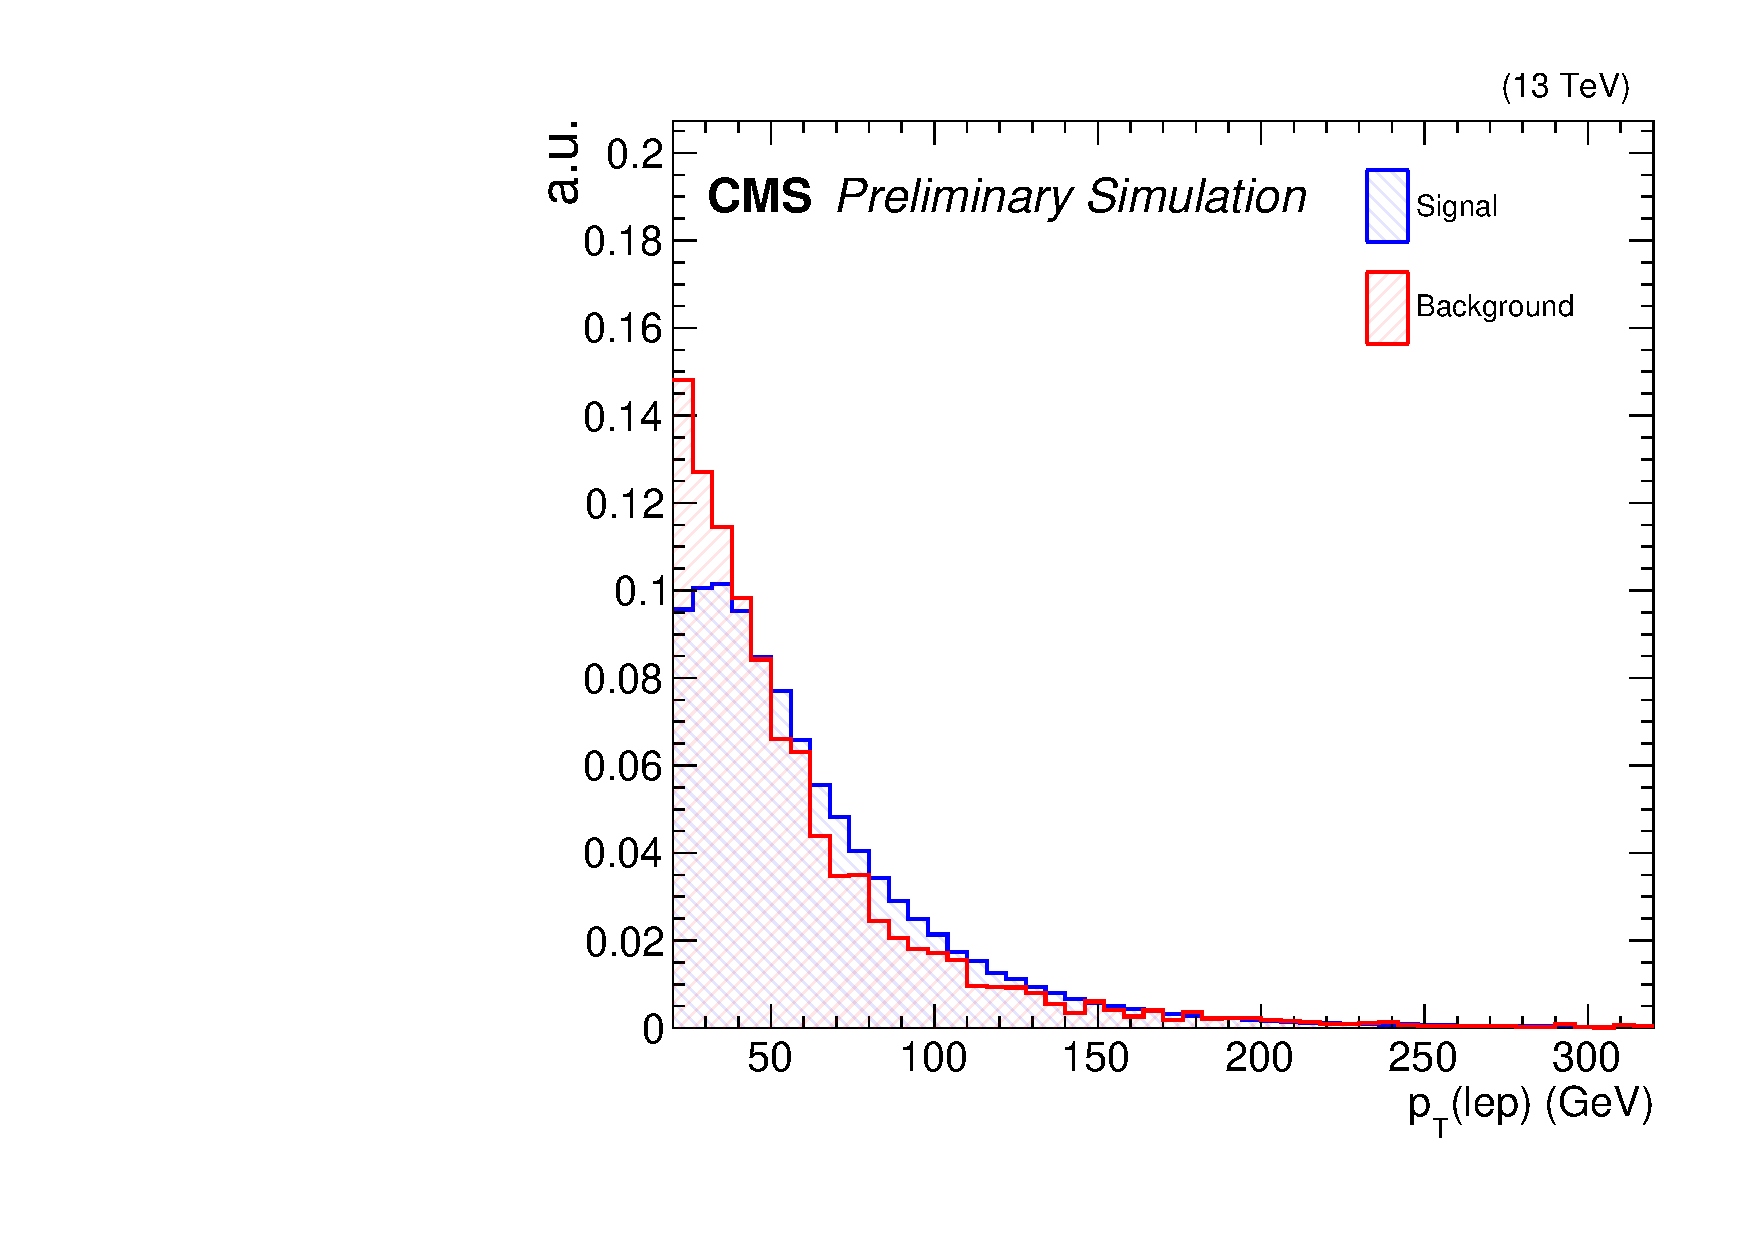
\includegraphics[width=0.24\textwidth]{pics/VH_sec/BDT_train_WH/BDT_lep_pt.pdf}
      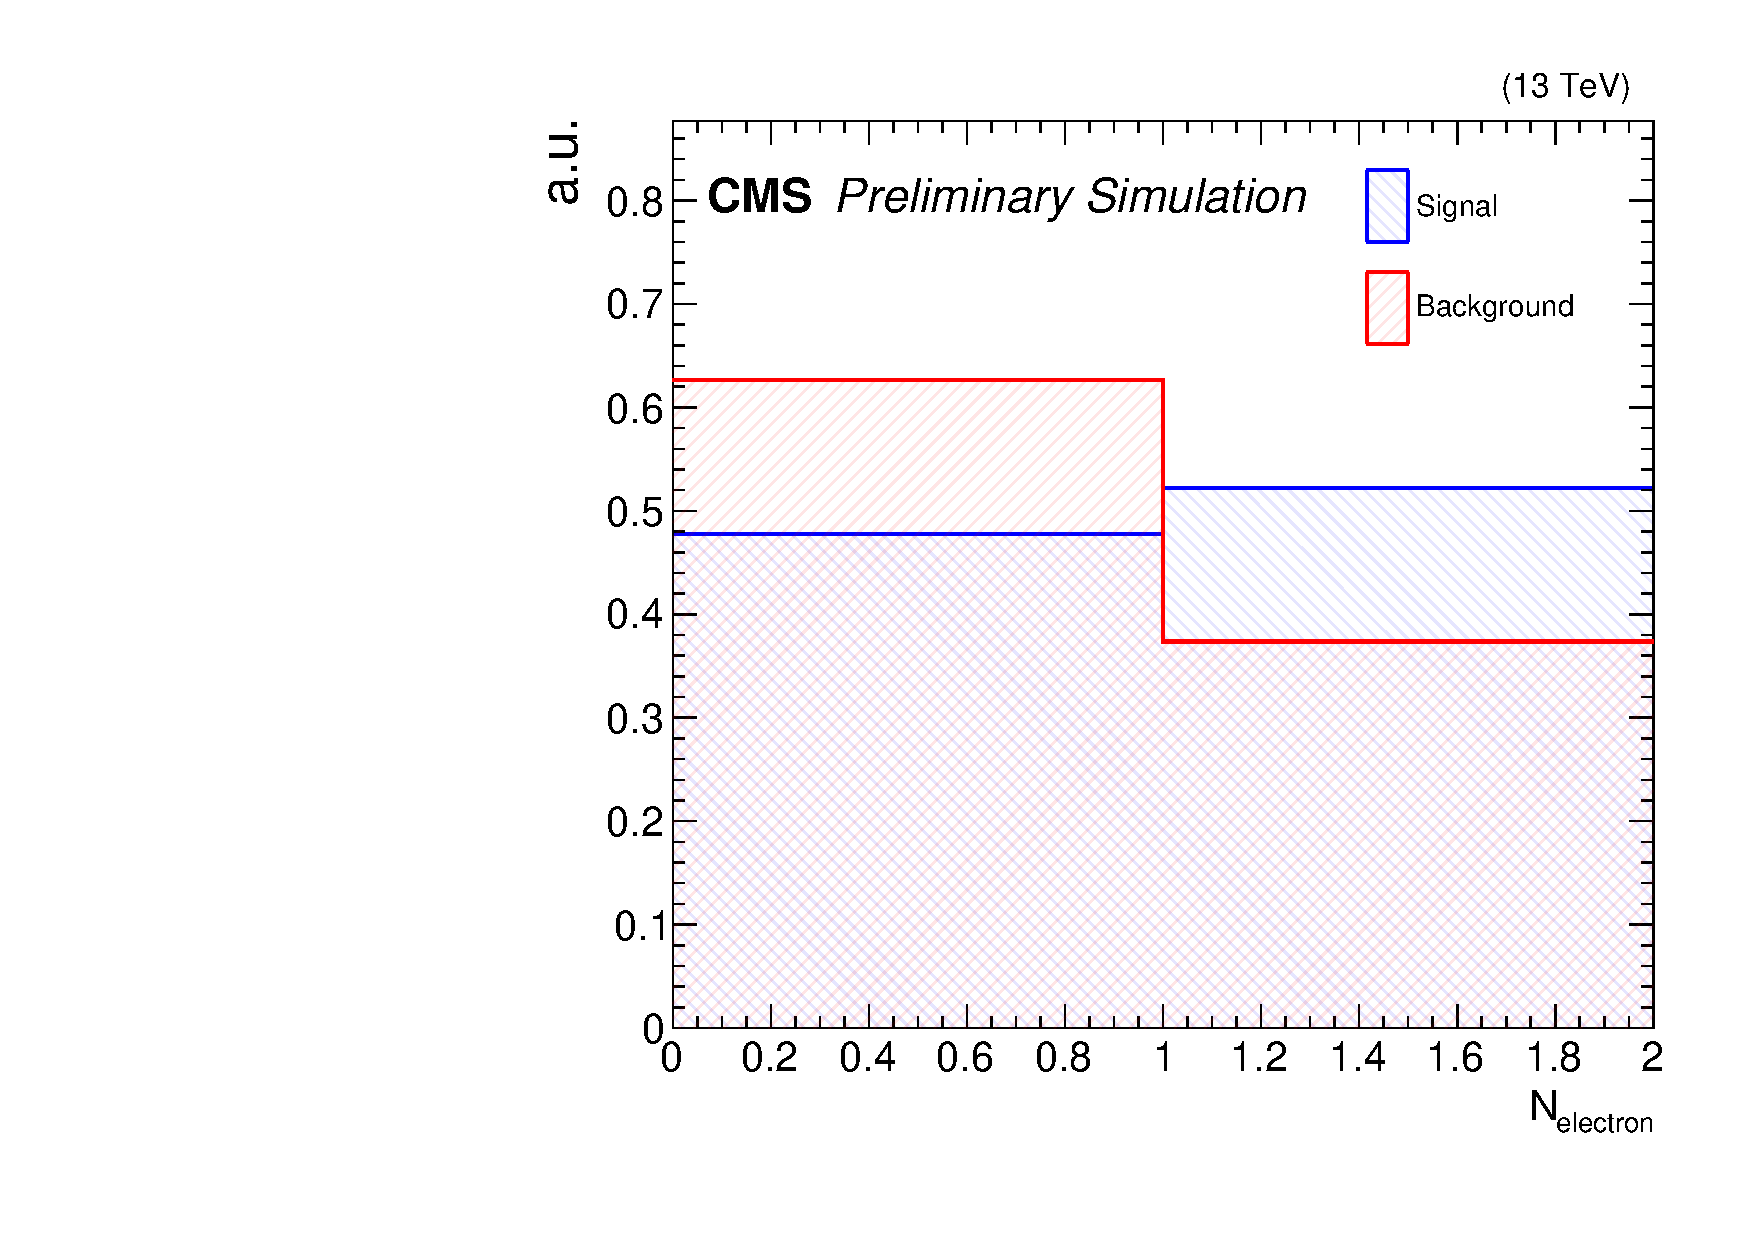
\includegraphics[width=0.24\textwidth]{pics/VH_sec/BDT_train_WH/BDT_nEles.pdf}
      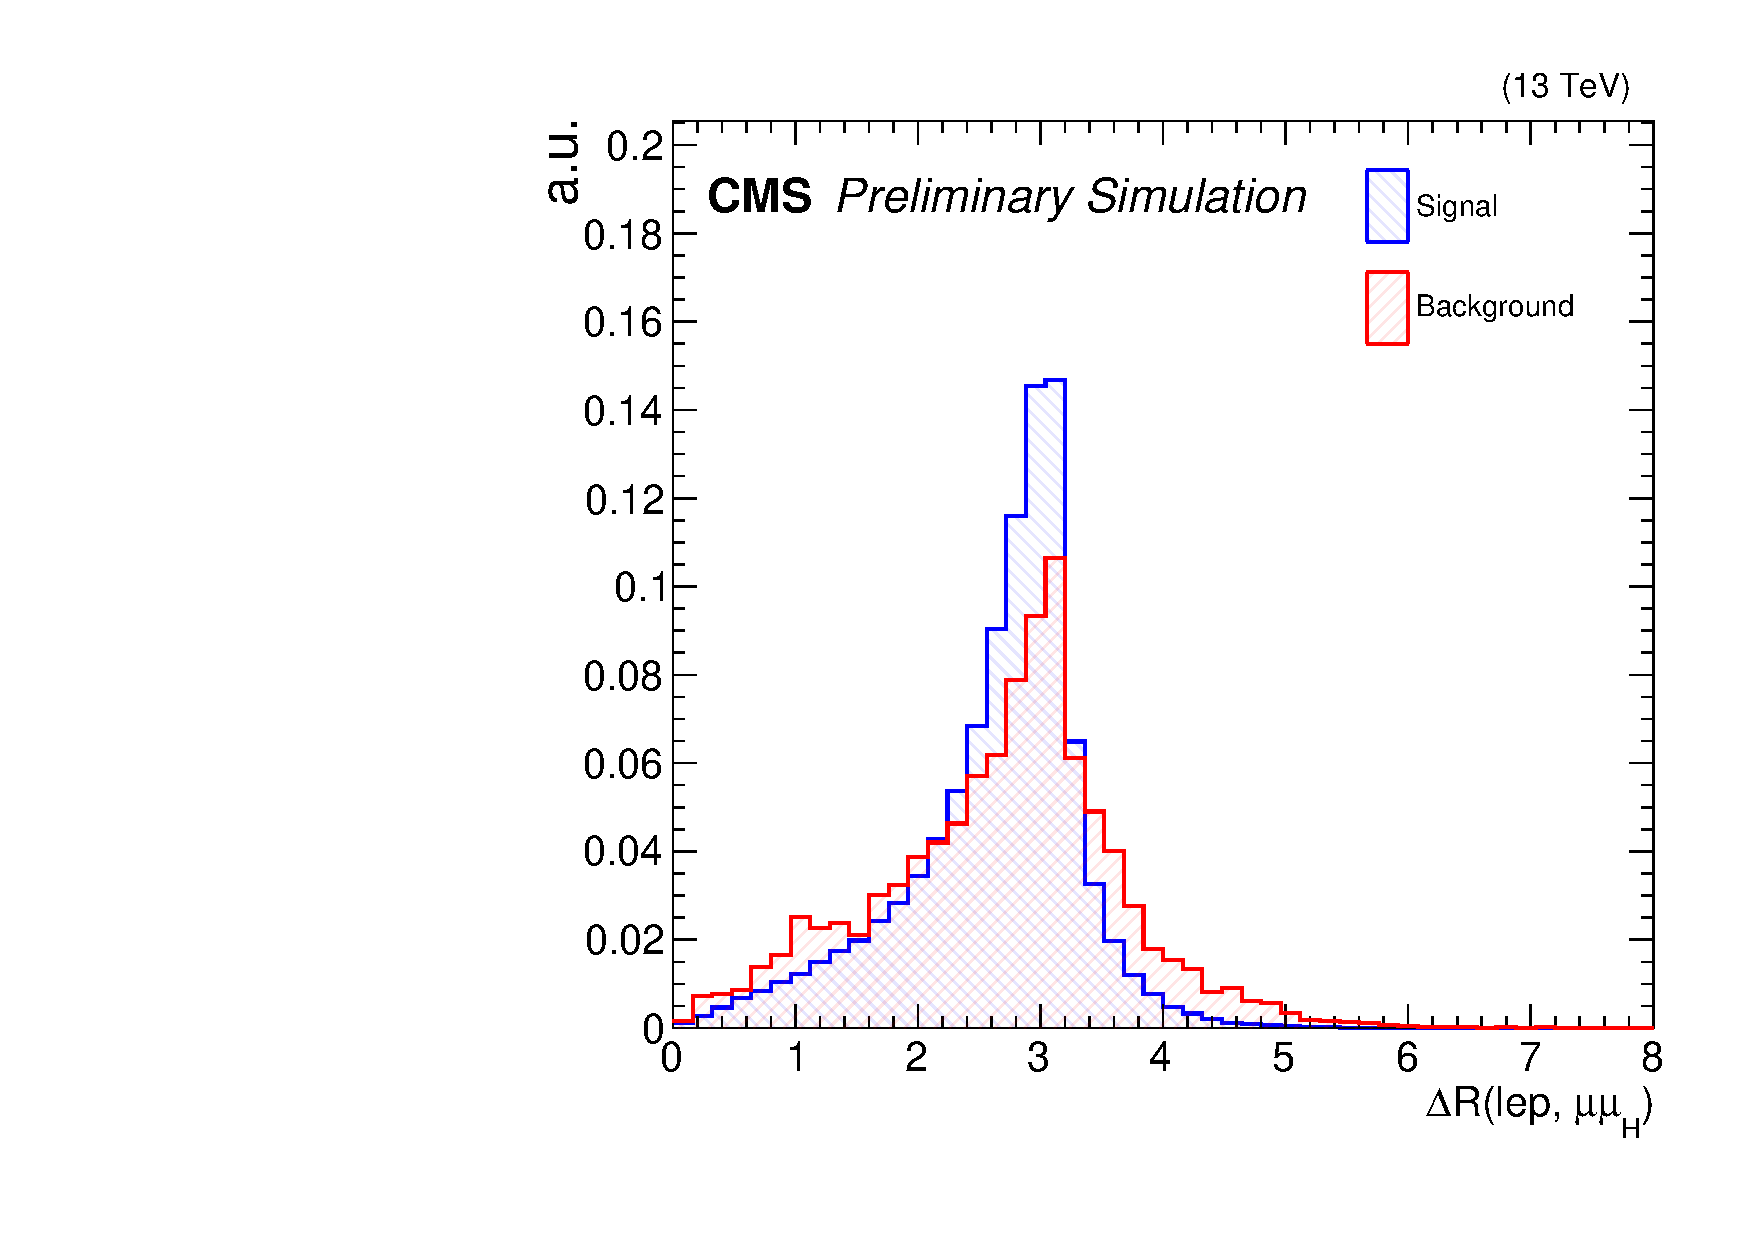
\includegraphics[width=0.24\textwidth]{pics/VH_sec/BDT_train_WH/BDT_lep_H_pair_dR.pdf}
      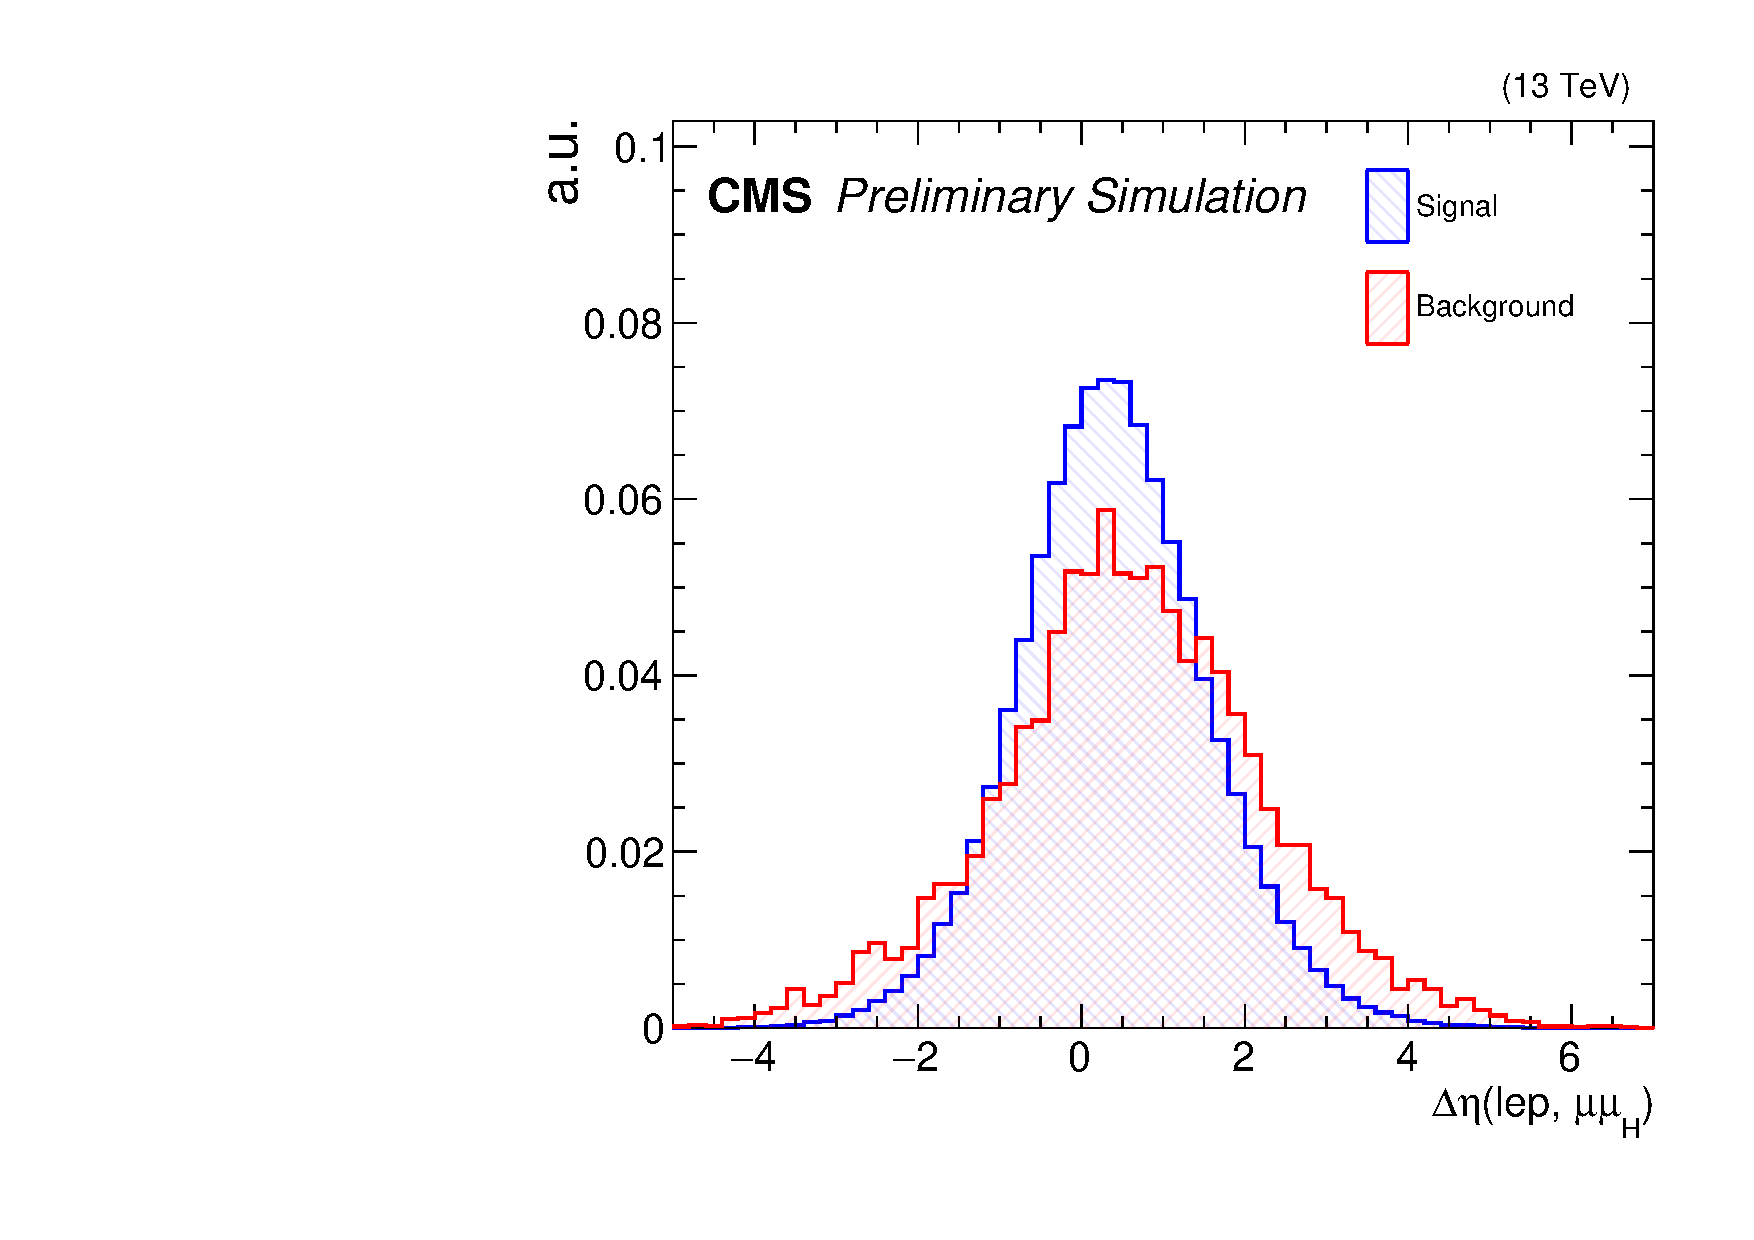
\includegraphics[width=0.24\textwidth]{pics/VH_sec/BDT_train_WH/BDT_lep_H_pair_dEta.pdf}
  
      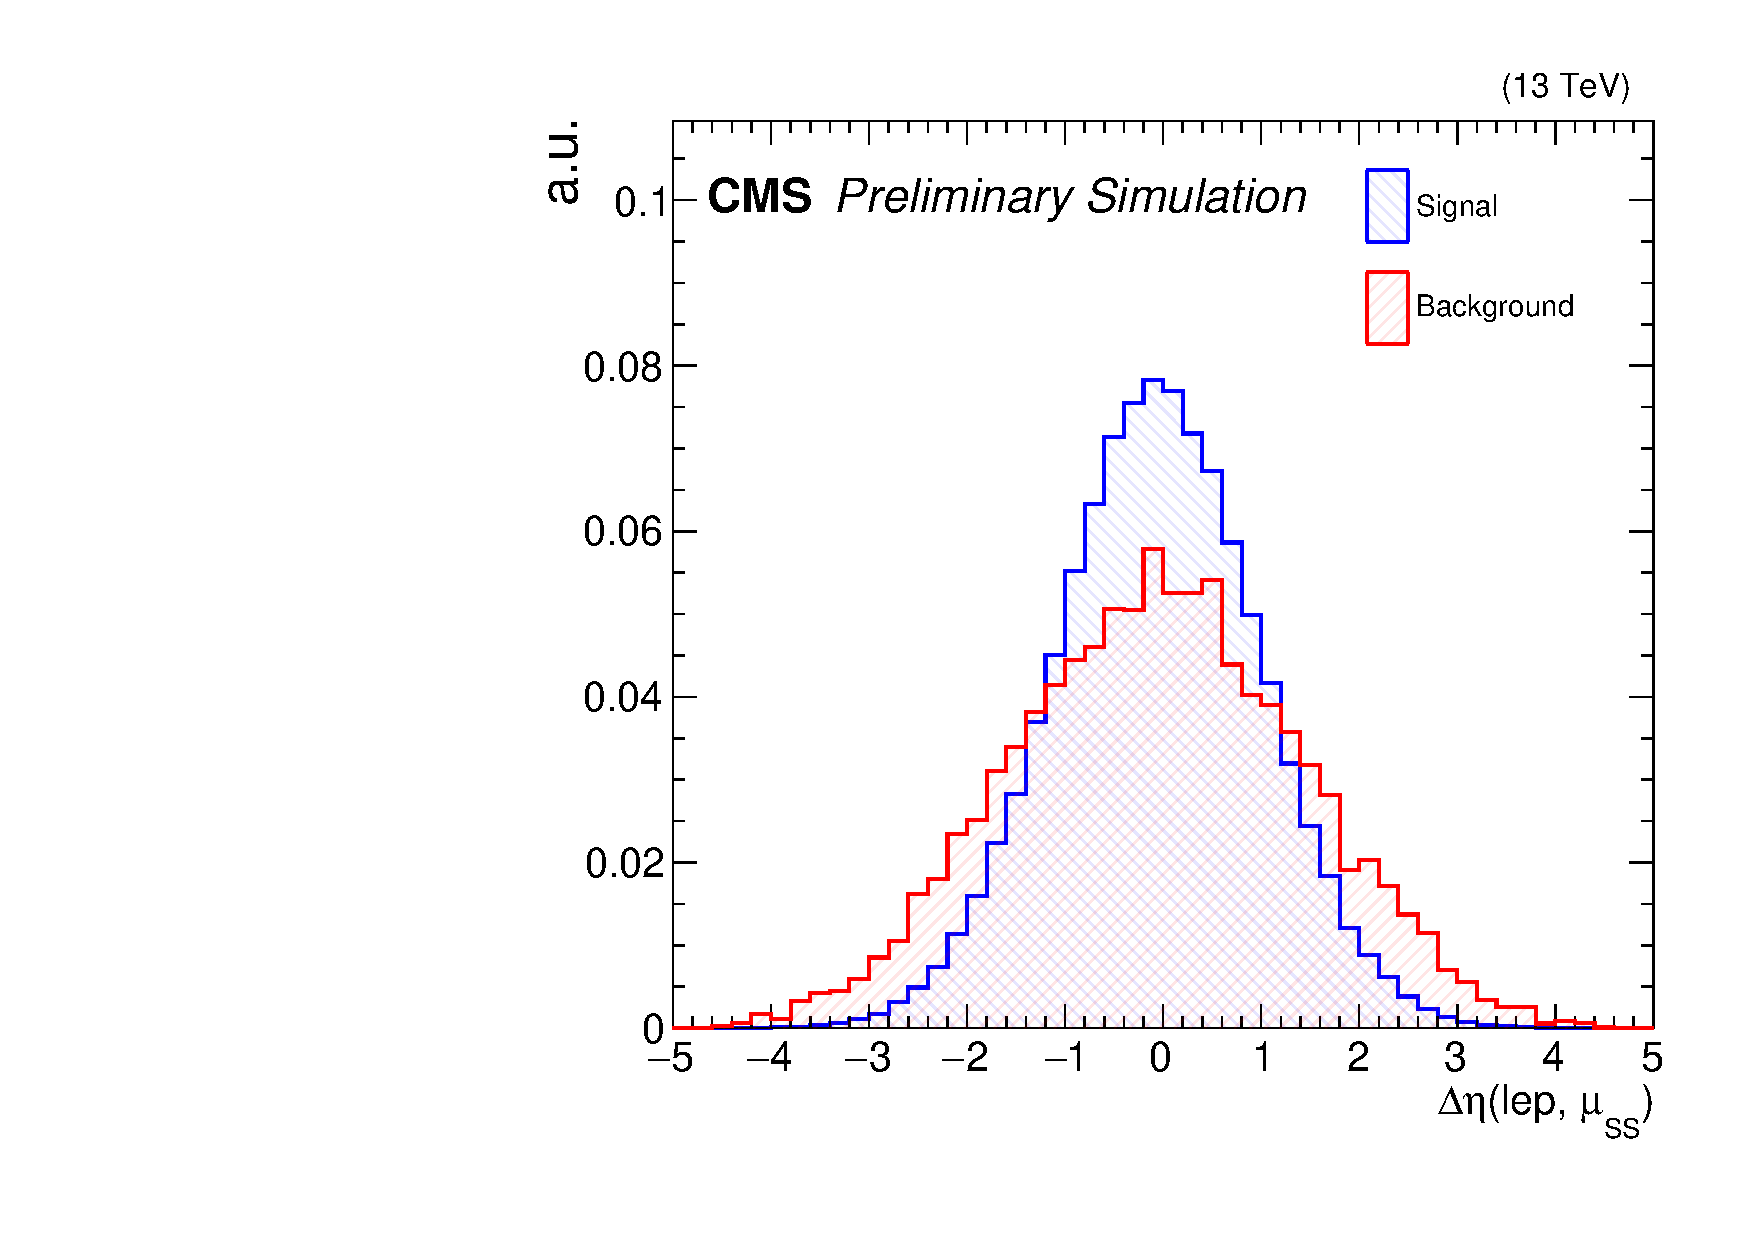
\includegraphics[width=0.24\textwidth]{pics/VH_sec/BDT_train_WH/BDT_lep_muSS_dEta.pdf}
      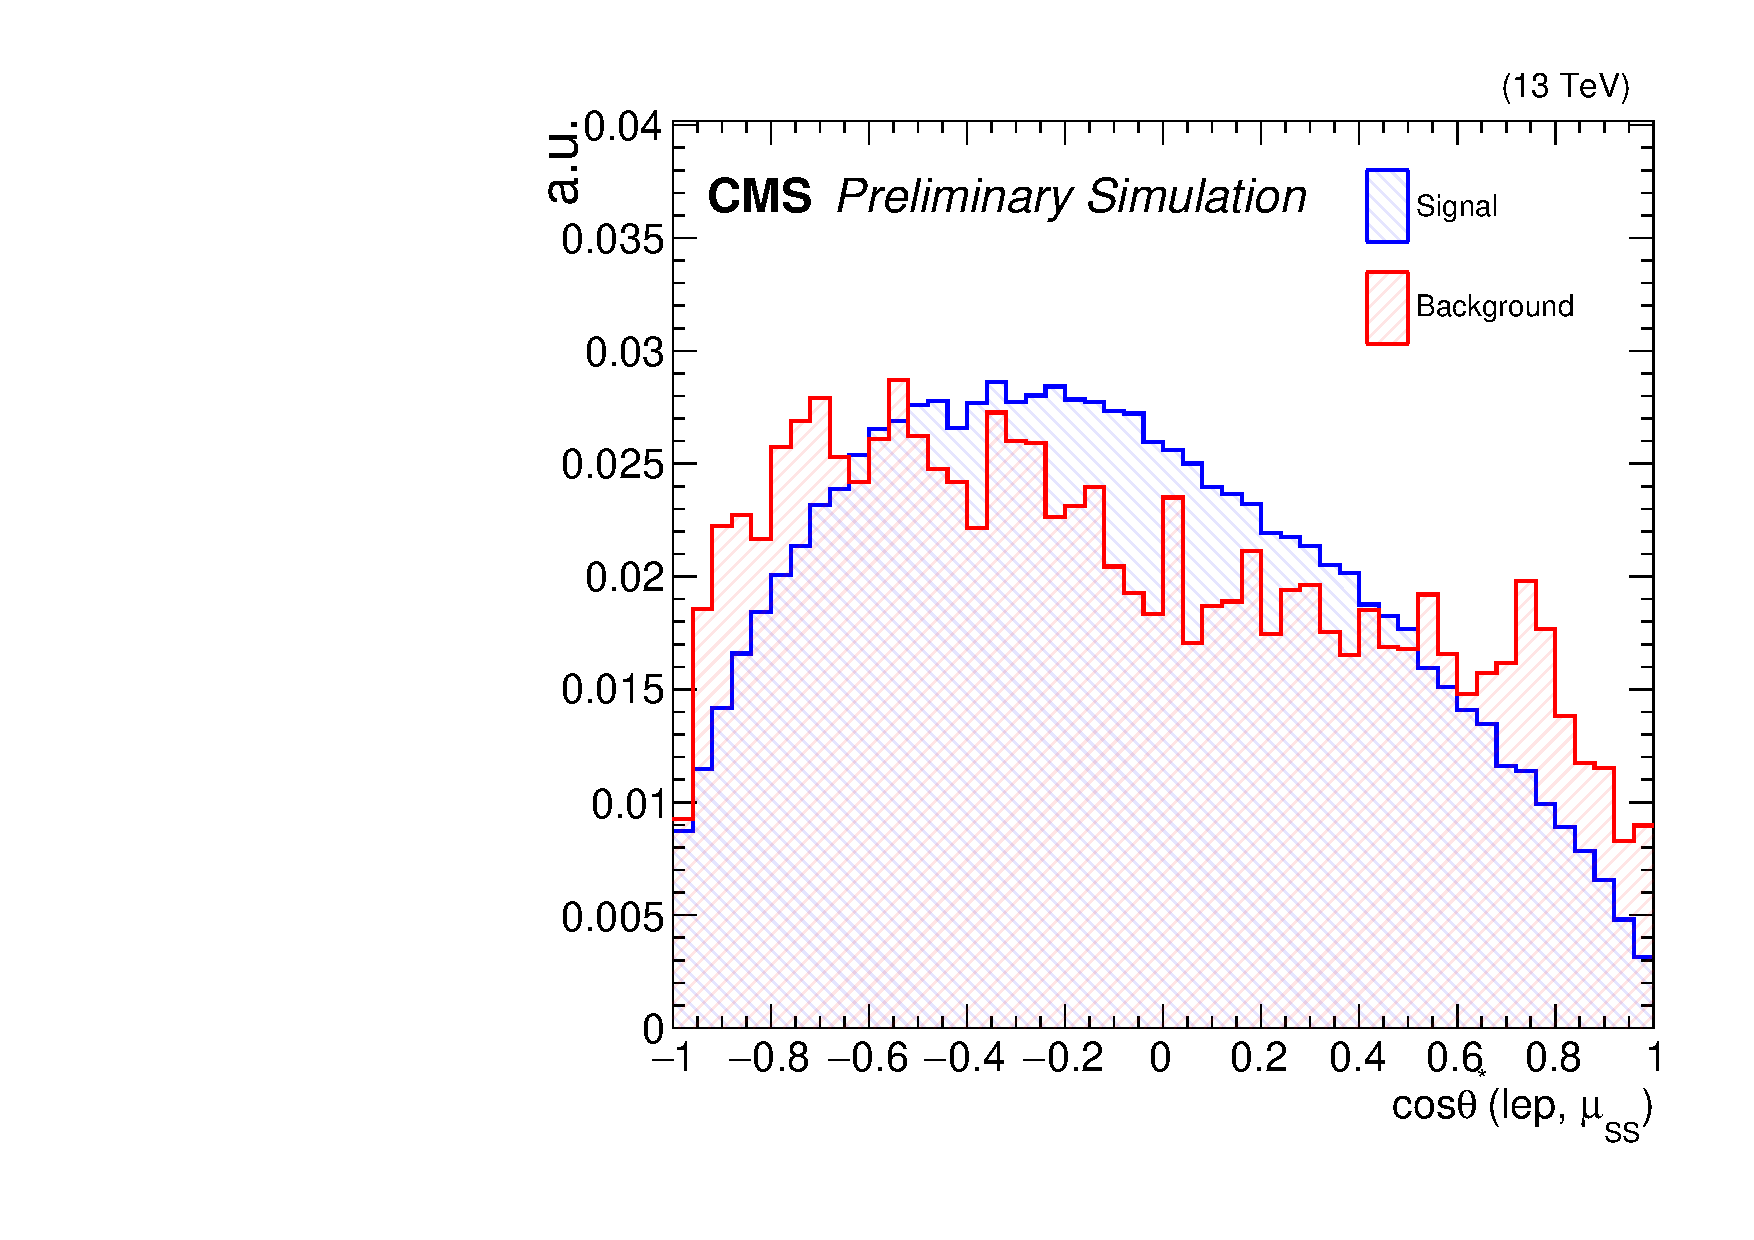
\includegraphics[width=0.24\textwidth]{pics/VH_sec/BDT_train_WH/BDT_lep_muSS_cosThStar.pdf}
      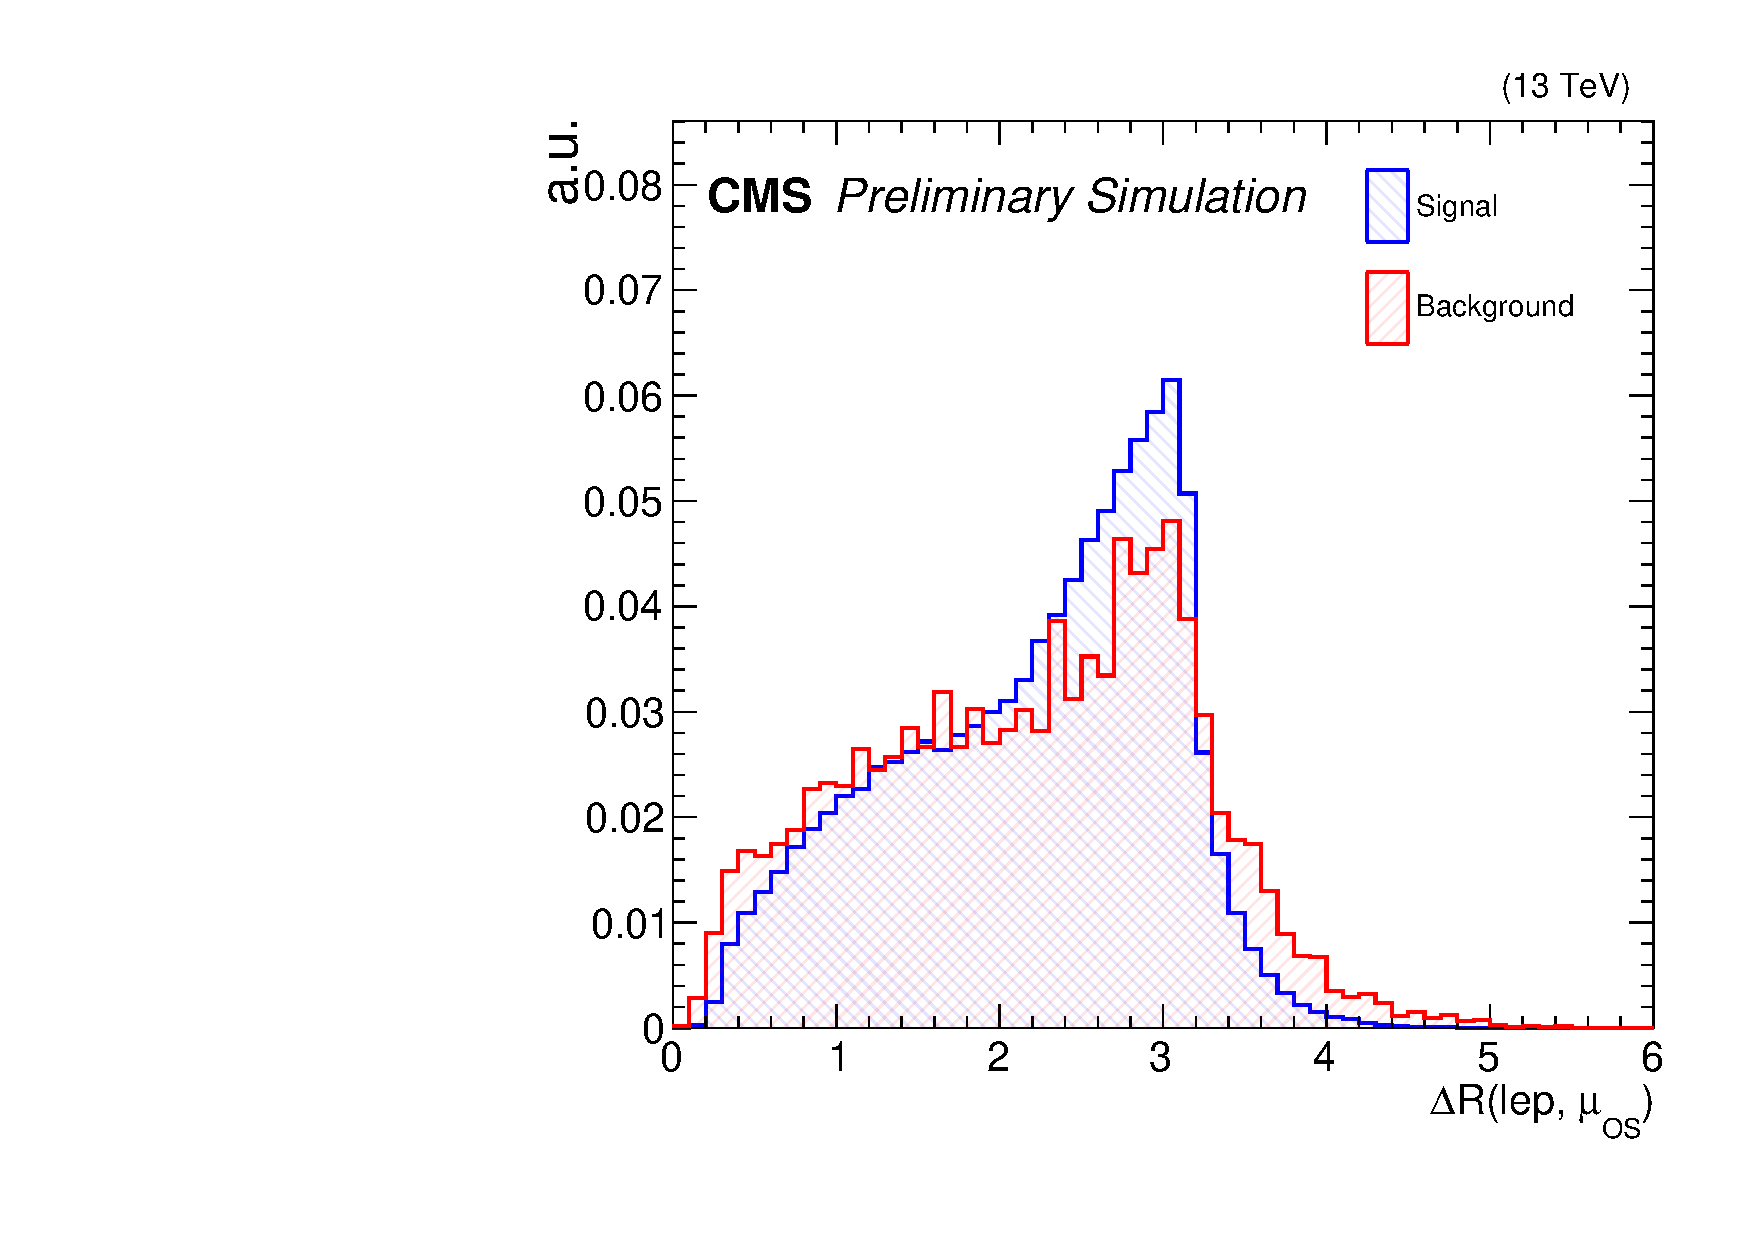
\includegraphics[width=0.24\textwidth]{pics/VH_sec/BDT_train_WH/BDT_lep_muOS_dR.pdf}
      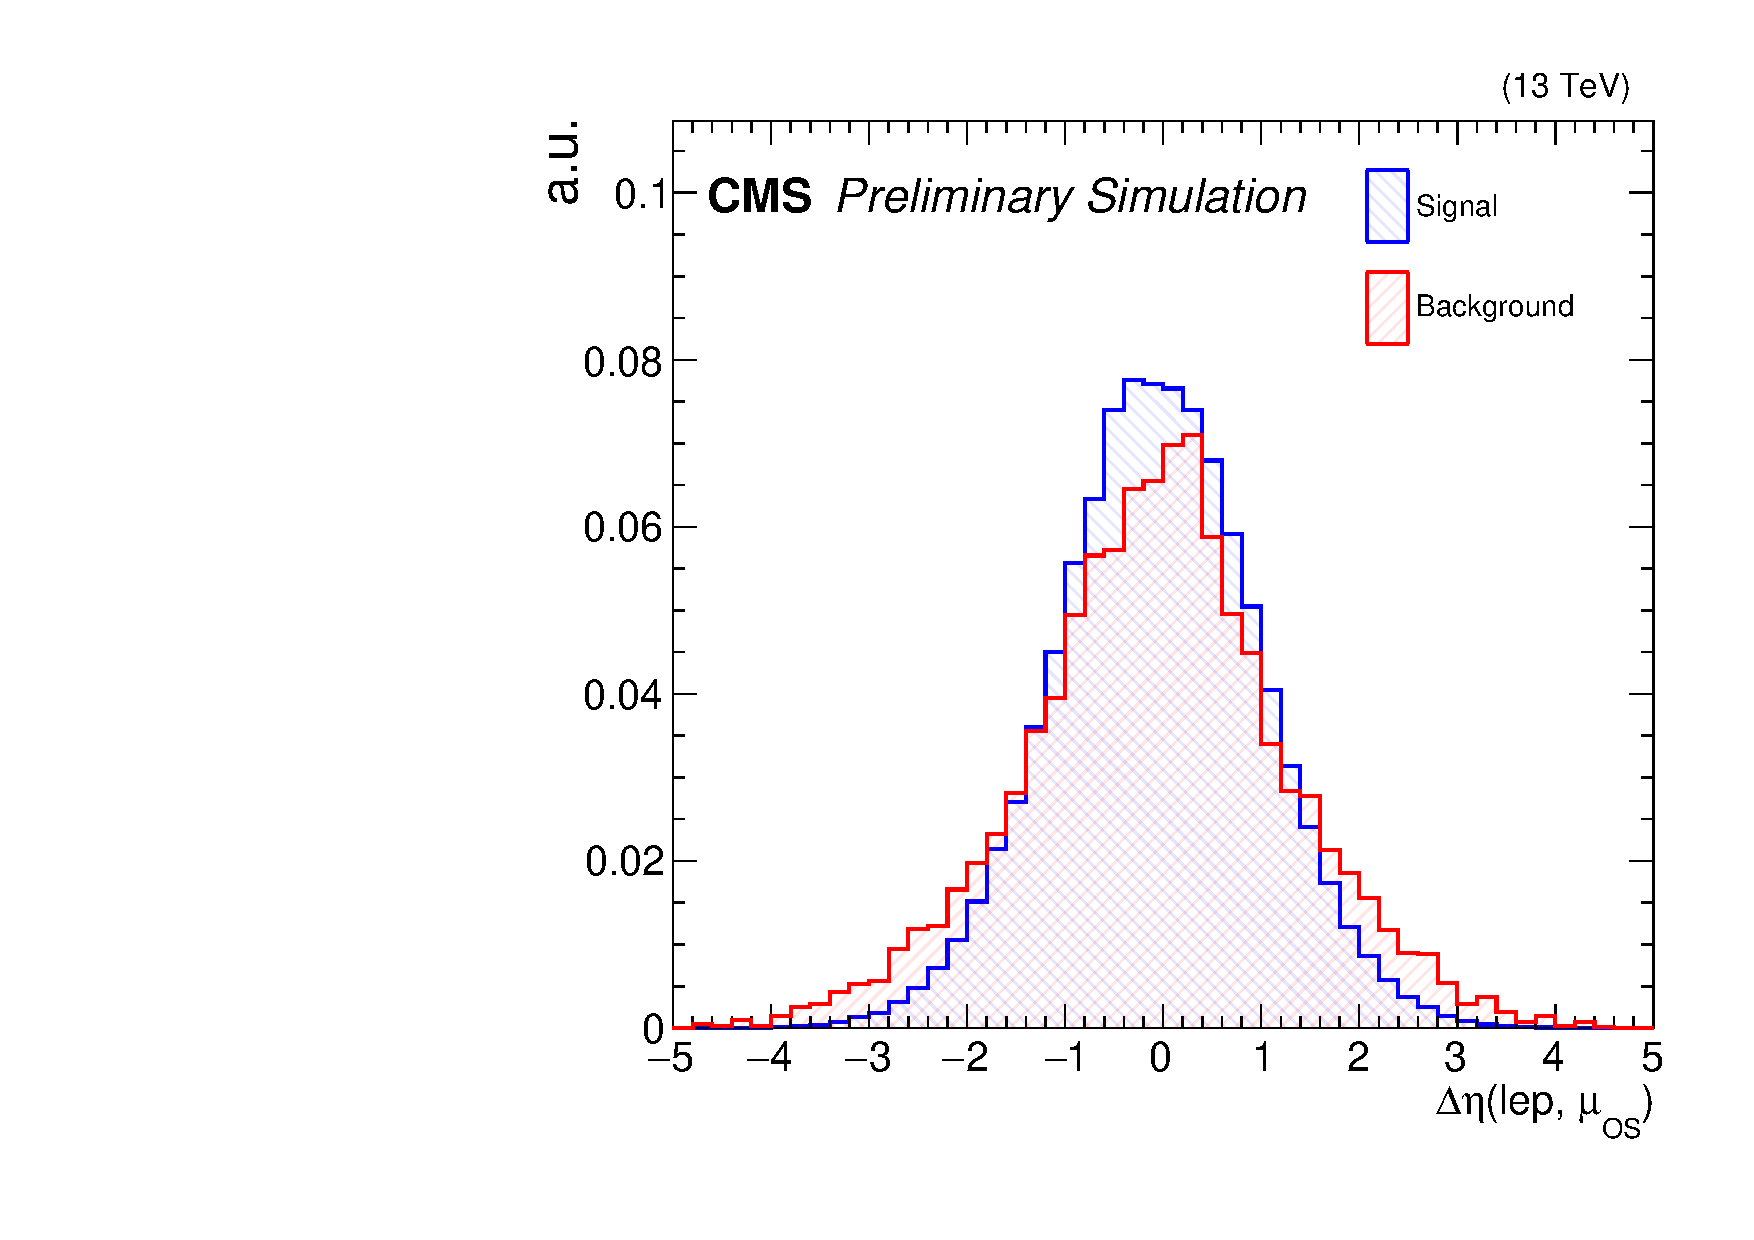
\includegraphics[width=0.24\textwidth]{pics/VH_sec/BDT_train_WH/BDT_lep_muOS_dEta.pdf}
  
      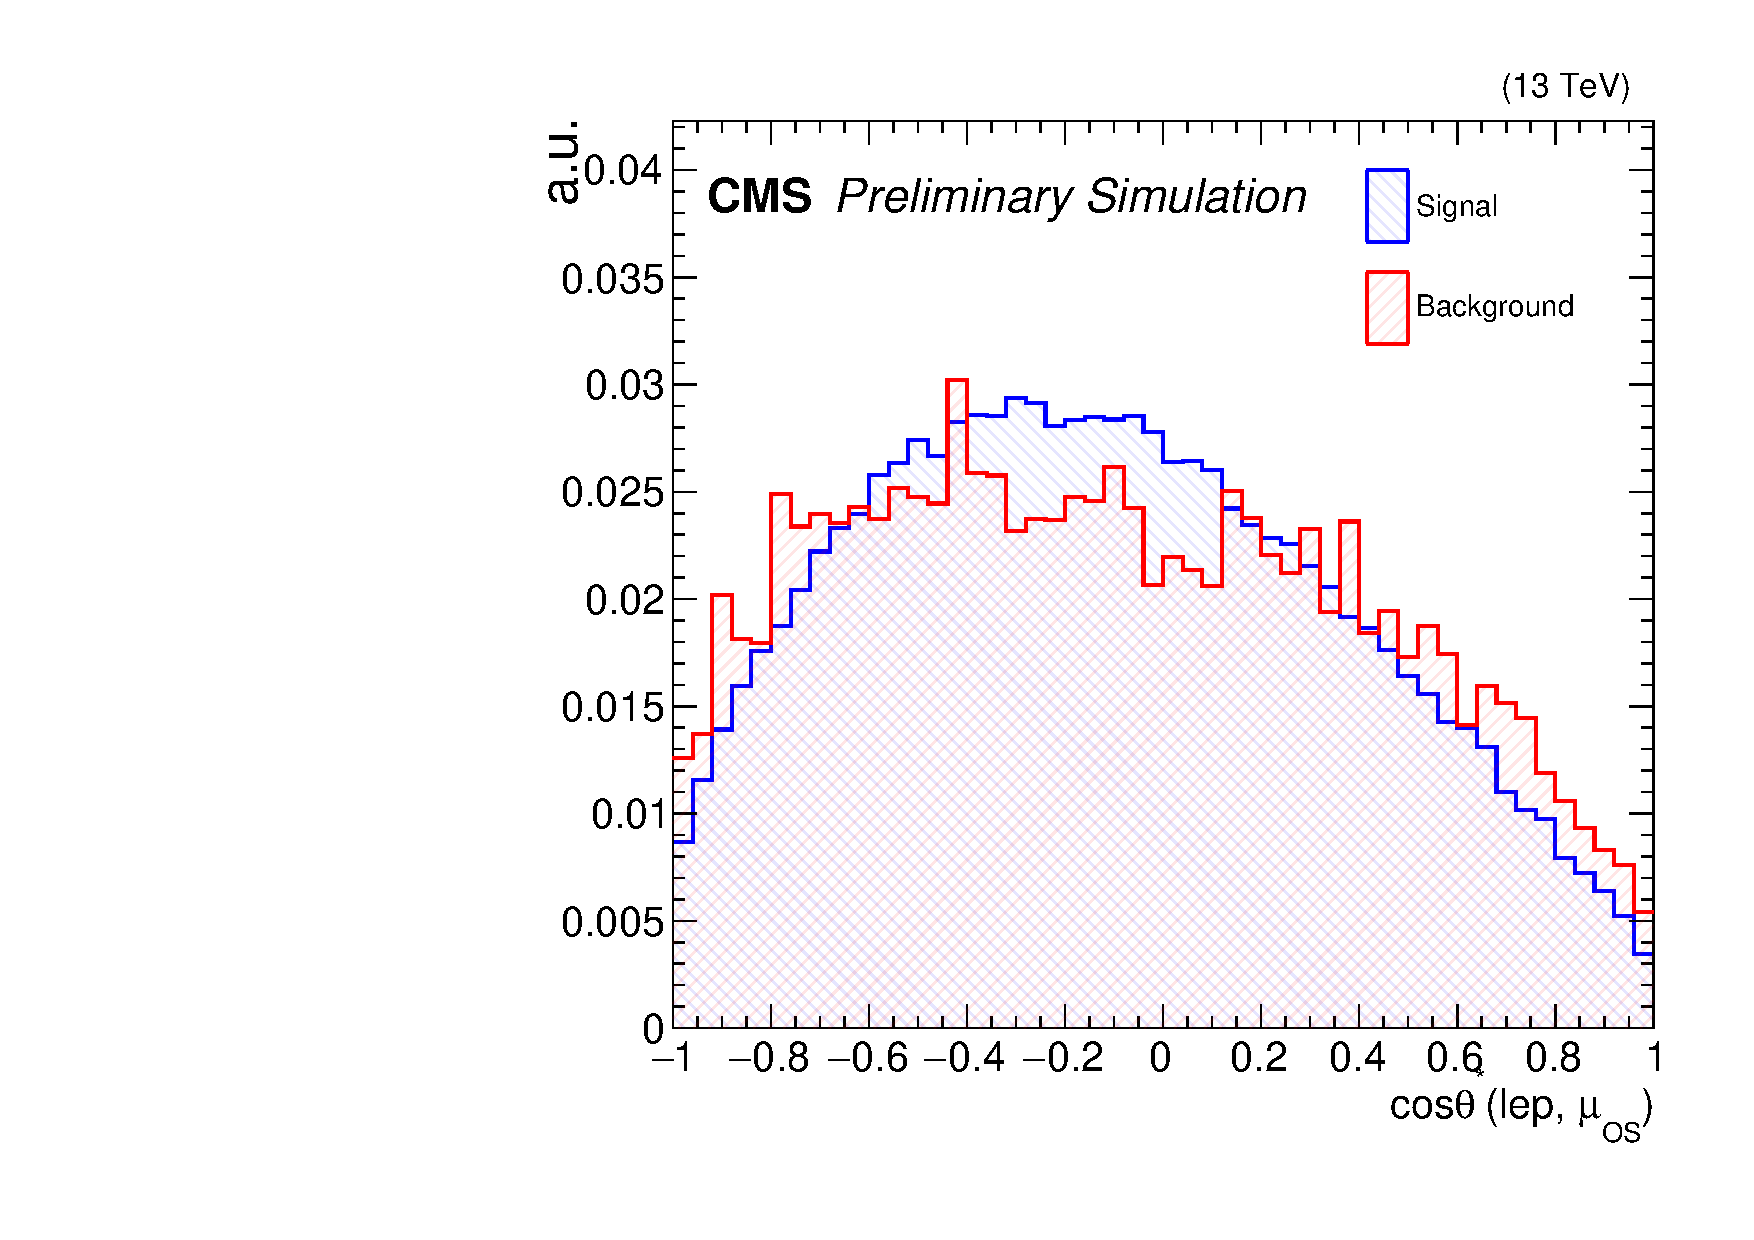
\includegraphics[width=0.24\textwidth]{pics/VH_sec/BDT_train_WH/BDT_lep_muOS_cosThStar.pdf}
      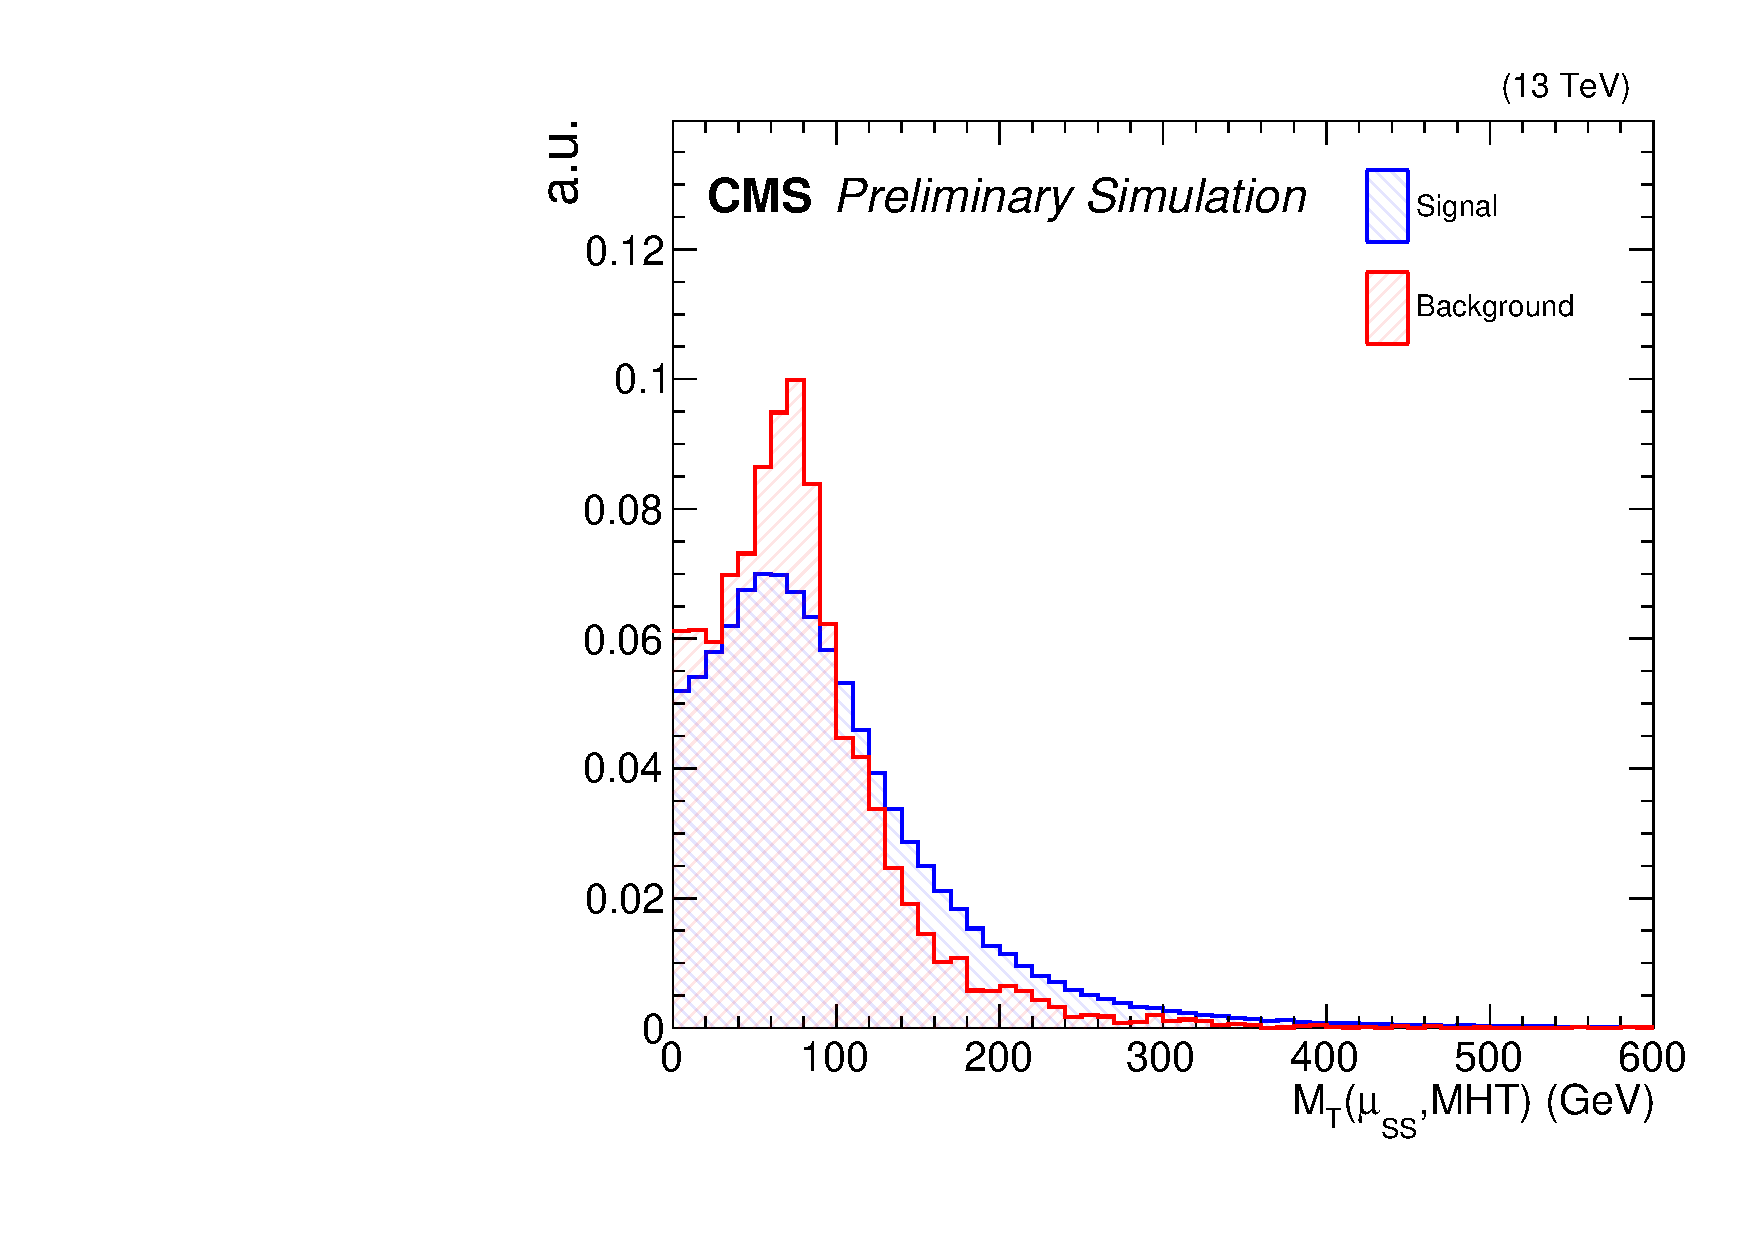
\includegraphics[width=0.24\textwidth]{pics/VH_sec/BDT_train_WH/BDT_muSS_MHT_MT.pdf}
      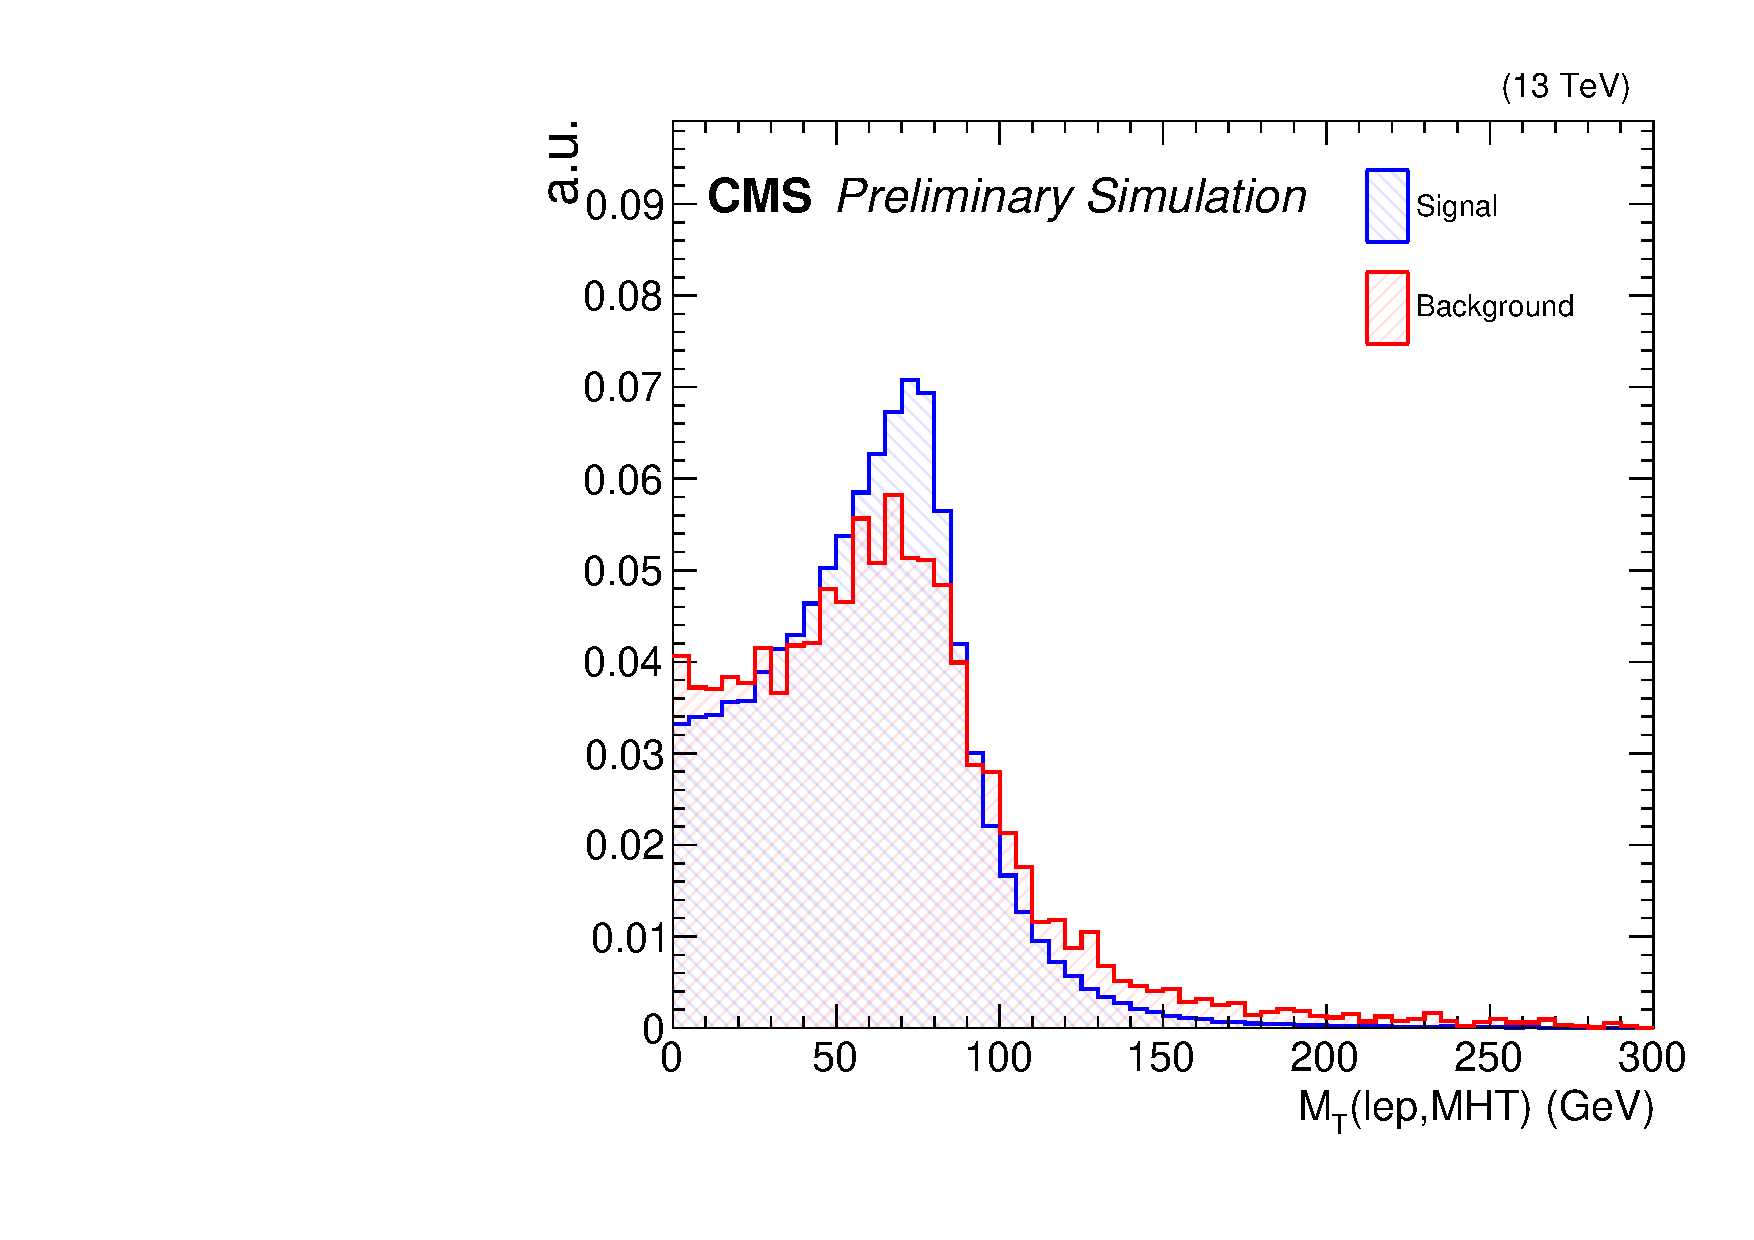
\includegraphics[width=0.24\textwidth]{pics/VH_sec/BDT_train_WH/BDT_lep_MHT_MT.pdf}
      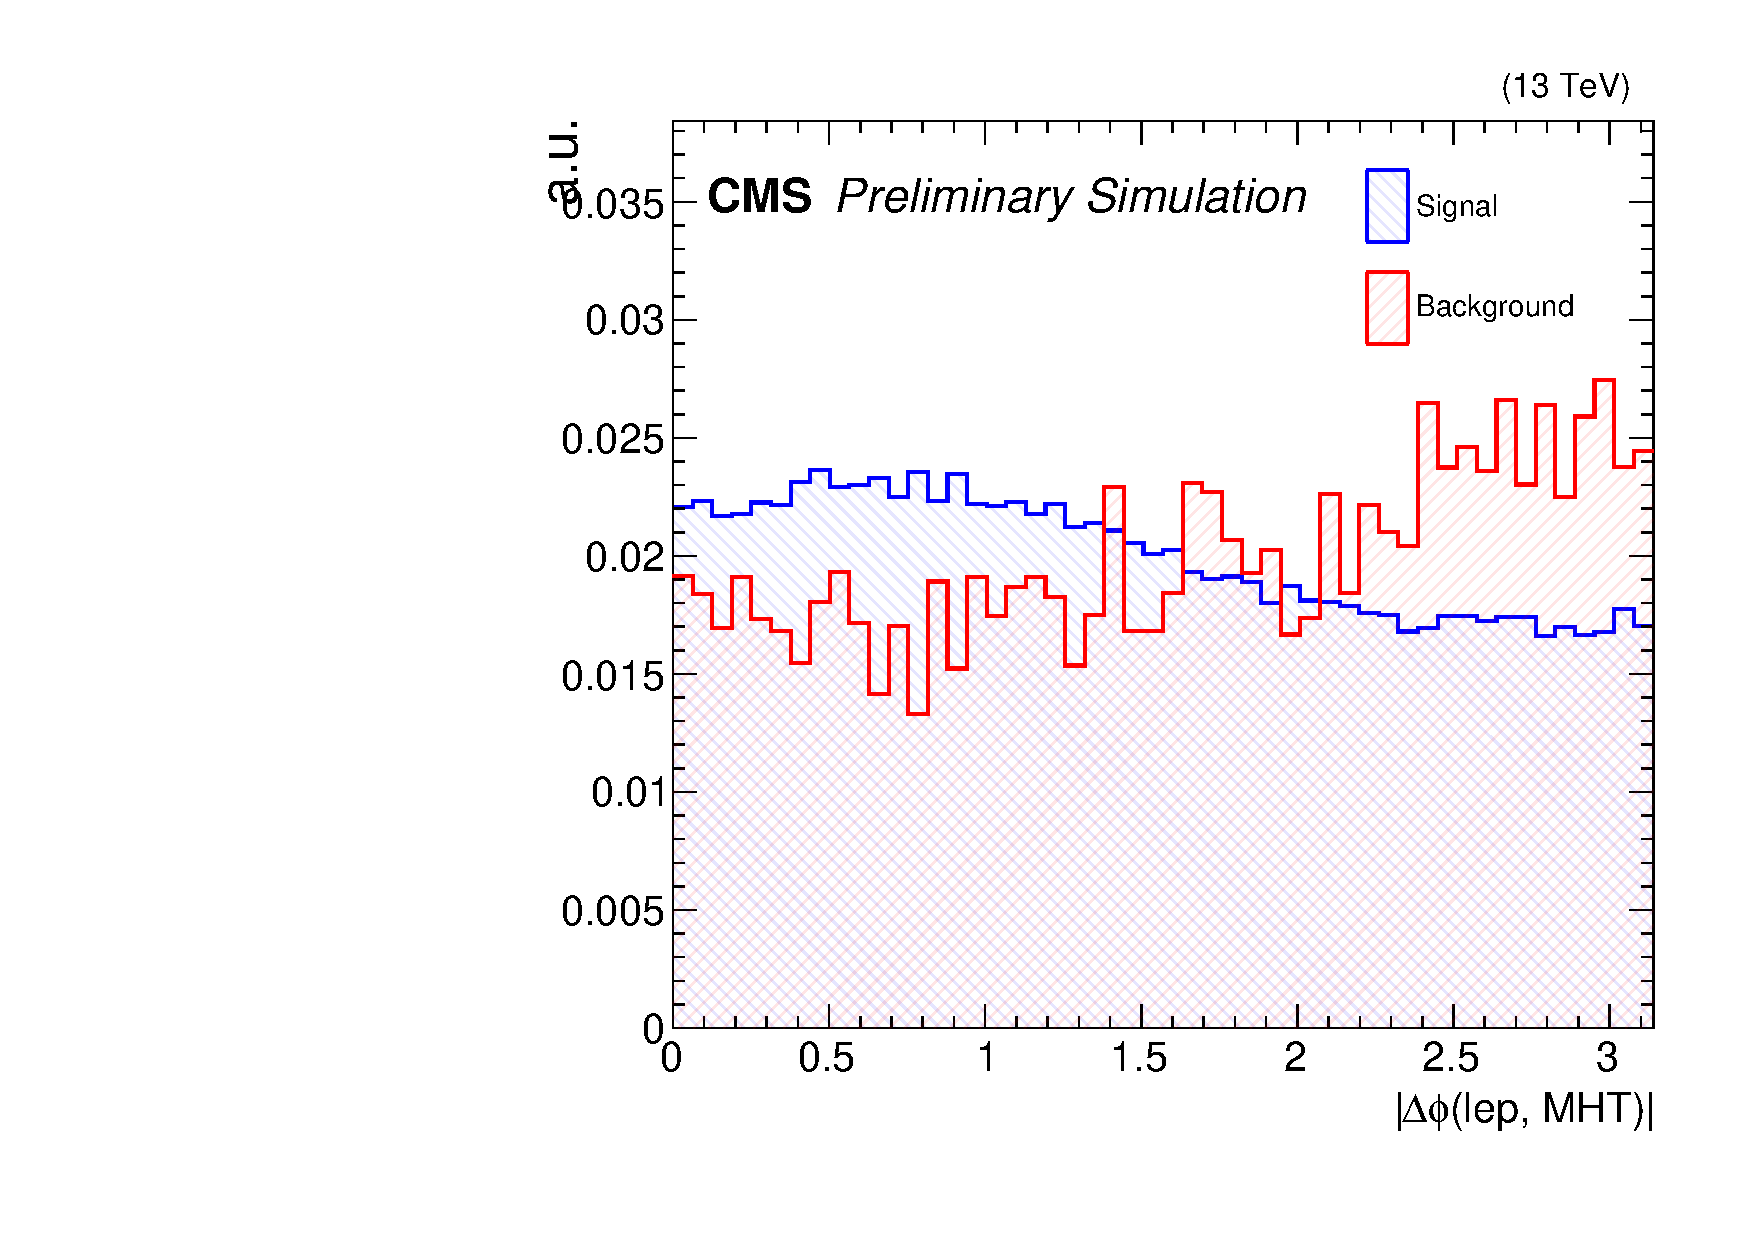
\includegraphics[width=0.24\textwidth]{pics/VH_sec/BDT_train_WH/BDT_lep_MHT_dPhi_abs.pdf}
      \caption{Input variables to the WH $\to 3\ell$ BDT, with signal in blue and background in red.}
      \label{fig:wh_bdt_vars}
  \end{figure*}
  
\subsection{BDT targeting \texorpdfstring{ZH $\to \ell\ell+\mu\mu$}{ZH to 4l} signal}\label{subsec:ZHlep_BDT}

After the event selection of the \ZH category, the background is almost purely composed of $\ZZ \to 4\ell$ and $\ggZZ \to 4 \ell$ processes. 
Other backgrounds, prompt or nonprompt, have negligible contribution in this channel. 
Both \ZZ and \ggZZ processes have the identical final states as the ZH signal. 
Apart from the dimuon mass, which is used in the last stage for 
signal extraction, the most distinct discrimination between the signal and the background 
lies in the helicity angles, between the leptons from the \PH (\PZ) decay, 
and between the \PH ($\PZ_{1}$) and the $\PZ_{2}$ bosons.

The input variables to the BDT are listed in Table~\ref{tab:zh_bdt_vars} and shown in Figure~\ref{fig:zh_bdt_vars}, 
among which, $\cos\theta^*(\mu\mu_{\PH},\ell\ell_{\PZ})$, the helicity angle between 
the Higgs candidate and the Z candidate, is one of the most discriminating. 
In the ZZ background process, a propagator Z boson ($\PZ_{0}$) couples to two Z bosons ($\PZ_{1}$ and $\PZ_{2}$),
which in turn decay to lepton pairs. Since Z bosons are spin-1 particles, in the $\PZ_{0} \to \PZ_{1}\PZ_{2}$ 
process, the direction of the decay is more likely to align with the direction of the momentum of $\PZ_{0}$.
Whereas in the ZH events, since the Higgs bosons are spin-0 particles, there is no preferred direction for 
the the $\PZ_{0} \to \PZ_{1}\PH$ decay. %\textcolor{red}{double check the distribution}.
A similar kinematic discrimination is also present in the helicity angle $\cos\theta^*(\mu_{1}, \mu_{2})$, 
between the \zmm decay and the \hmm decay, 
where in the \PZ decay the muons prefer to align with the momentum of their parent and in the \PH decay they follow a flat distribution in $\cos\theta^*$. 
However, in this analysis, because of the acceptance of the CMS detector, 
the distribution of $\cos\theta^*(\mu_{1}, \mu_{2})$ is sculpted and turns out not very different between signal and background. 
This variable is included in the initial training and later discarded during the variable trimming process.

Similar to the WH BDT training, as described in Section~\ref{subsec:WHlep_BDT}, 
the training is performed with simulated samples from all eras in Run2. The training is performed in the mass 
window of $110 ~\GeV{} < \mmm < 150 ~\GeV{}$.  This training was performed prior to the production
of ggZH signal samples, so only qqZH samples are used as signal events. 
Signal samples with different Higgs boson mass assumptions, $\mh = 120, 125, 130$ GeV, are used. 
Signal events are only used if the candidate $\mu\mu$ pair truly originates from the Higgs boson decay.  
Signal events are weighted by 1/$\sigma(\mmm^{H})$.
Events with $ee+\mu\mu$ and $\mu\mu+\mu\mu$ are used together in the training, 
but can be distinguished with the "lepton flavor" as one of the input variables.  
To increase the statistics of training events, a relaxed lepMVA cut is used in the training.
Even so, there is no nonprompt background component passing the loosened selection.

The BDT output and the ROC curve are shown in Figure~\ref{fig:zh_BDT_out},
in which the BDT performs the same on training and testing samples, indicating no over-training.
Distributions of the BDT input variables are shown in Figure~\ref{fig:zh_bdt_vars}.

\begin{table*}[!htb]
    \centering
    \captionsetup{justification=justified}
    \topcaption{List of input variables used to train the signal-background
      separation BDT in the ZH category. In this table, $\mu\mu_{\PH}$ is the Higgs candidate,
      and $\ell\ell_{\PZ}$ is the \PZ candidate.}
    \begin{tabular}{lc}
    \hline
      Variable                                     & Description  \\
    \hline
      \pt$(\mu\mu_{\PH})$                          & \pt of the Higgs candidate\\
      $|\eta(\mu\mu_{\PH})|$                       & $|\eta|$ of the Higgs candidate \\
      $|\Delta\phi(\mu\mu_{\PH})|$                 & $|\Delta\phi|$ between the muons in the Higgs candidate\\
      M$(\ell\ell_{\PZ})$                          & invariant mass of the Z candidate\\
      \pt($\ell\ell_{\PZ}$)                        & \pt of the Z candidate\\
      $|\eta(\ell\ell_{\PZ})|$                     & $|\eta|$ of the Z candidate\\
      $\Delta$R$(\ell\ell_{\PZ})$                  & $\Delta$R between the leptons in the Z candidate\\
      lepton flavor                                & flavor of the Z candidate lepton pair\\
      $\cos\theta^*(\mu\mu_{\PH},\ell\ell_{\PZ})$  & cosine helicity angle between the Higgs and the Z candidates\\
      $\Delta\eta(\mu\mu_{\PH},\ell\ell_{\PZ})$    & $\Delta\eta$ between the Higgs and the Z candidates\\
    \hline
    \end{tabular}
    \label{tab:zh_bdt_vars}
\end{table*}

\begin{figure*}[!htb]
    \centering
    \captionsetup{justification=justified}
    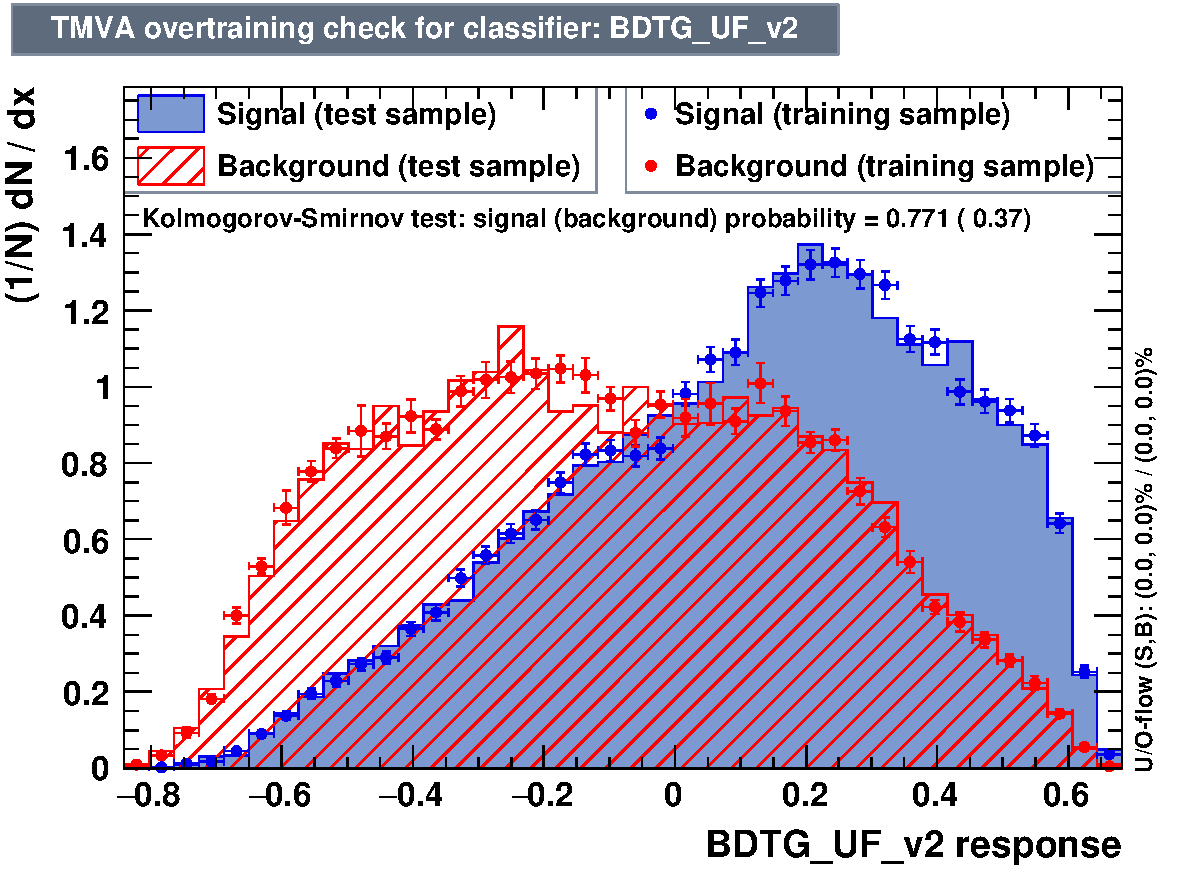
\includegraphics[width=0.50\textwidth]{pics/VH_sec/BDT_train_ZH/ZH_BDT_overtrain.pdf}
    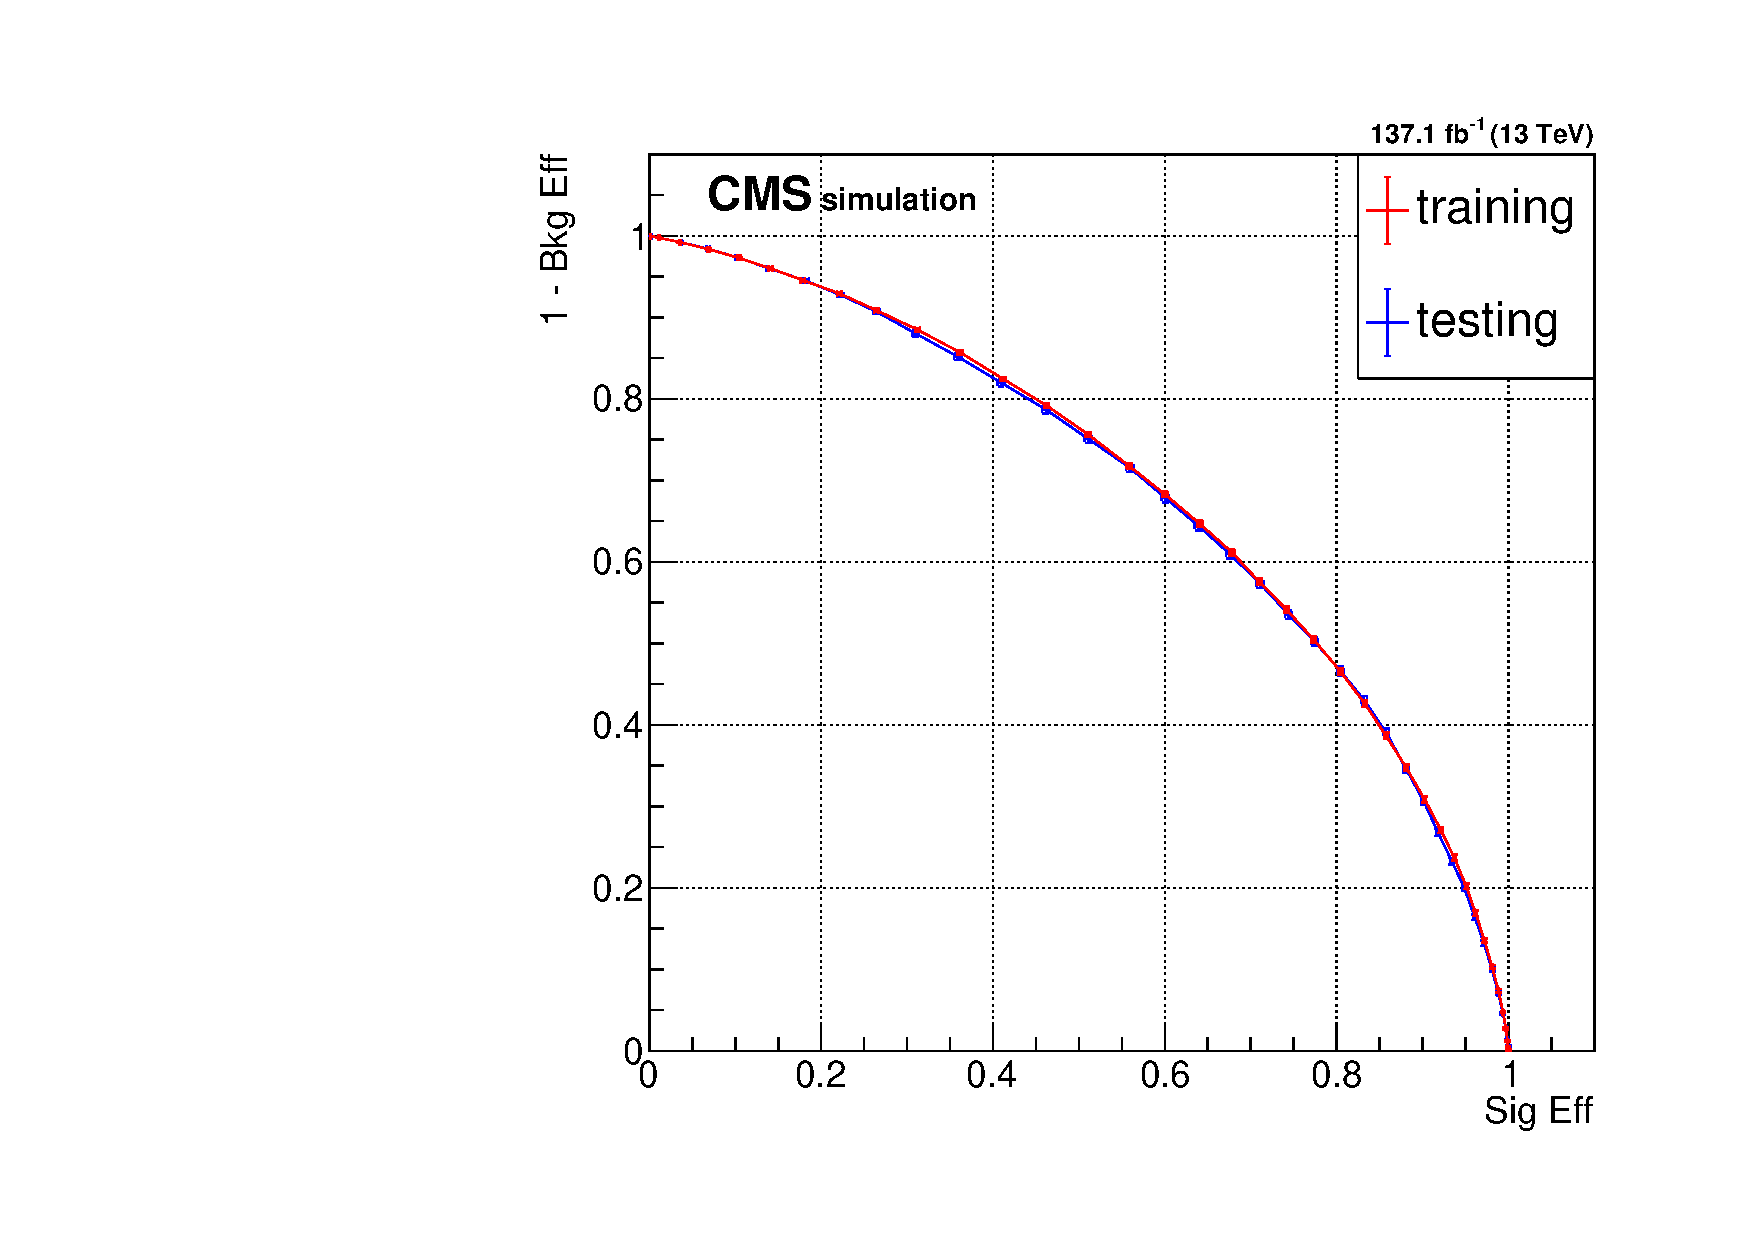
\includegraphics[width=0.43\textwidth]{pics/VH_sec/BDT_train_ZH/ZH_BDT_ROC.pdf}
    \caption{Plots of the performance of the ZH $\to 4\ell$ BDT.
             On the left, the BDT output score, with signal in blue and background in red.  
             On the right, the receiver operating characteristic (ROC) curve, 
             with training in red and testing in blue.}
    \label{fig:zh_BDT_out}
\end{figure*}

\begin{figure*}[!htb]
    \centering
    \captionsetup{justification=justified}
    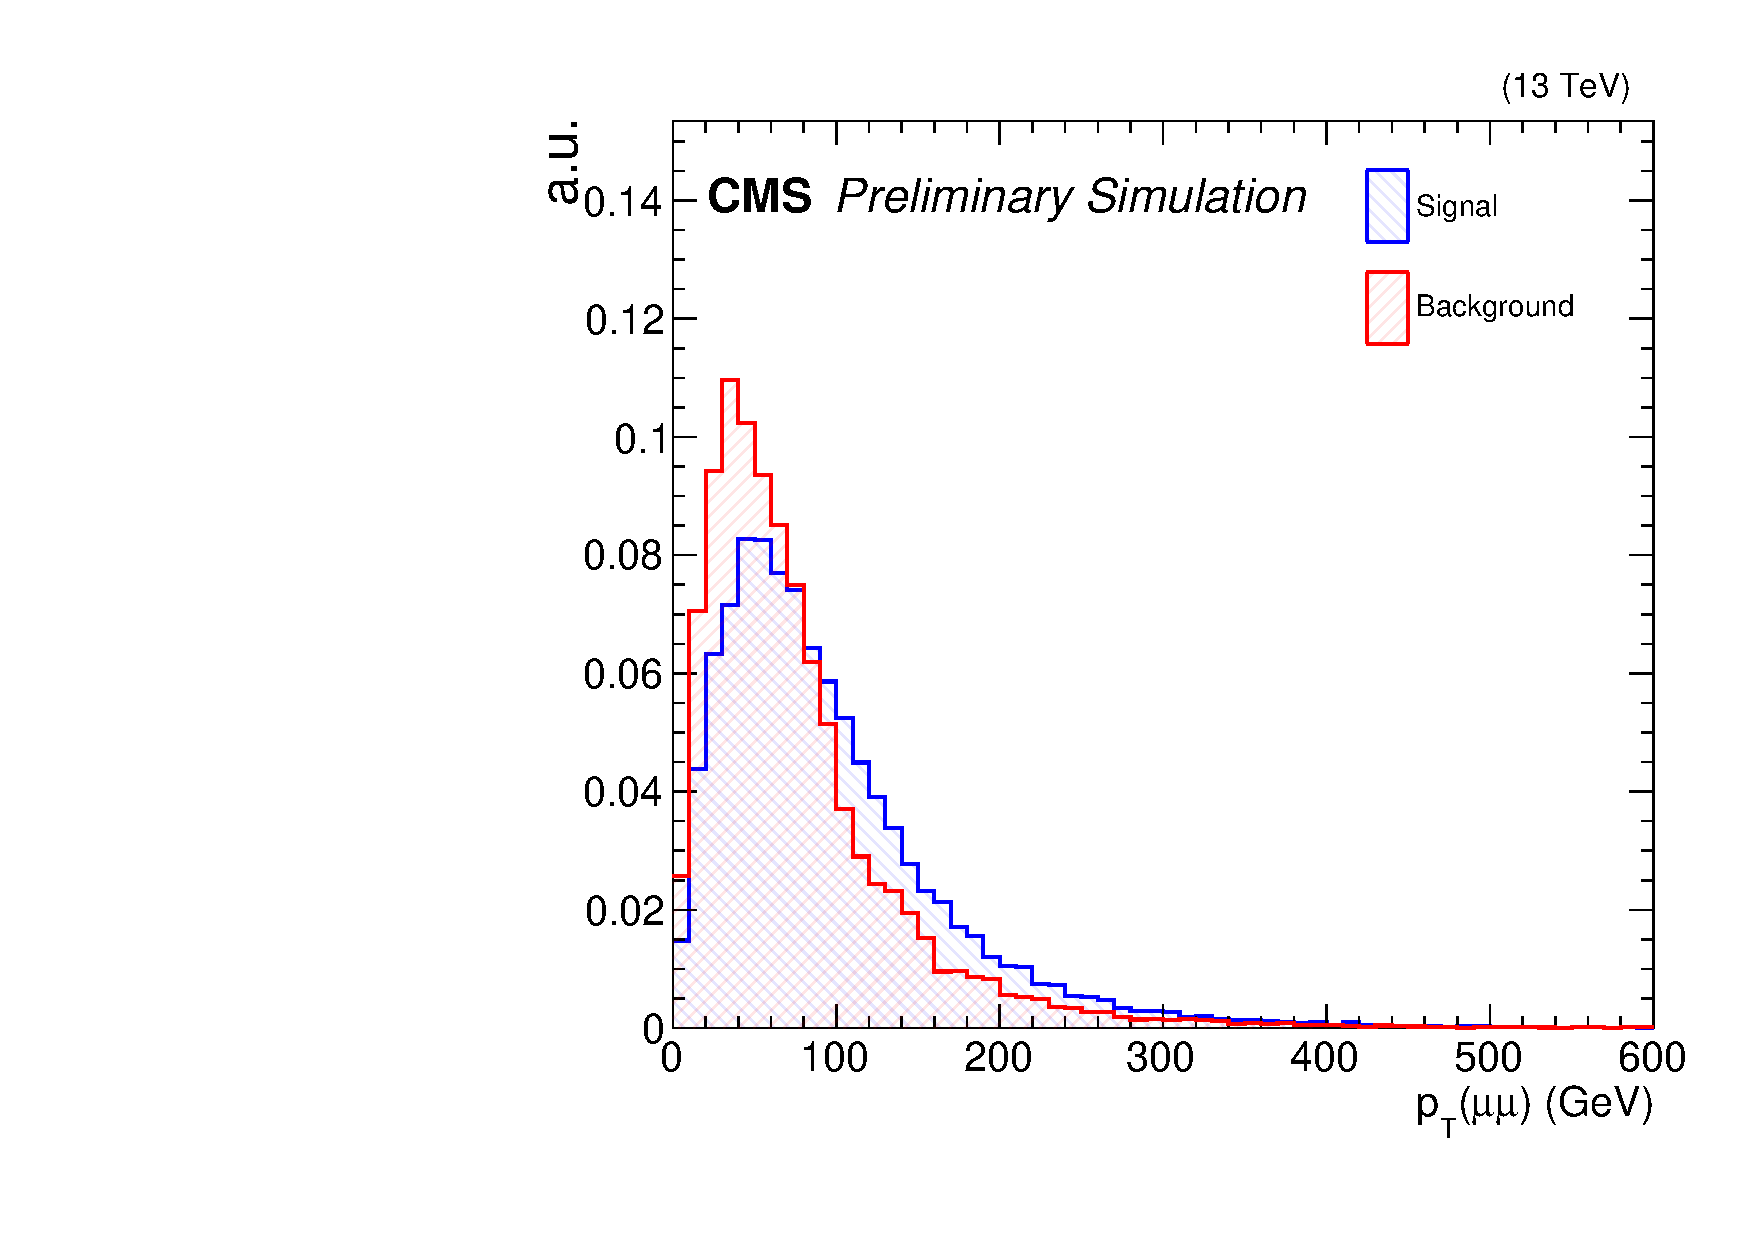
\includegraphics[width=0.24\textwidth]{pics/VH_sec/BDT_train_ZH/BDT_dimu_pt.pdf} 
    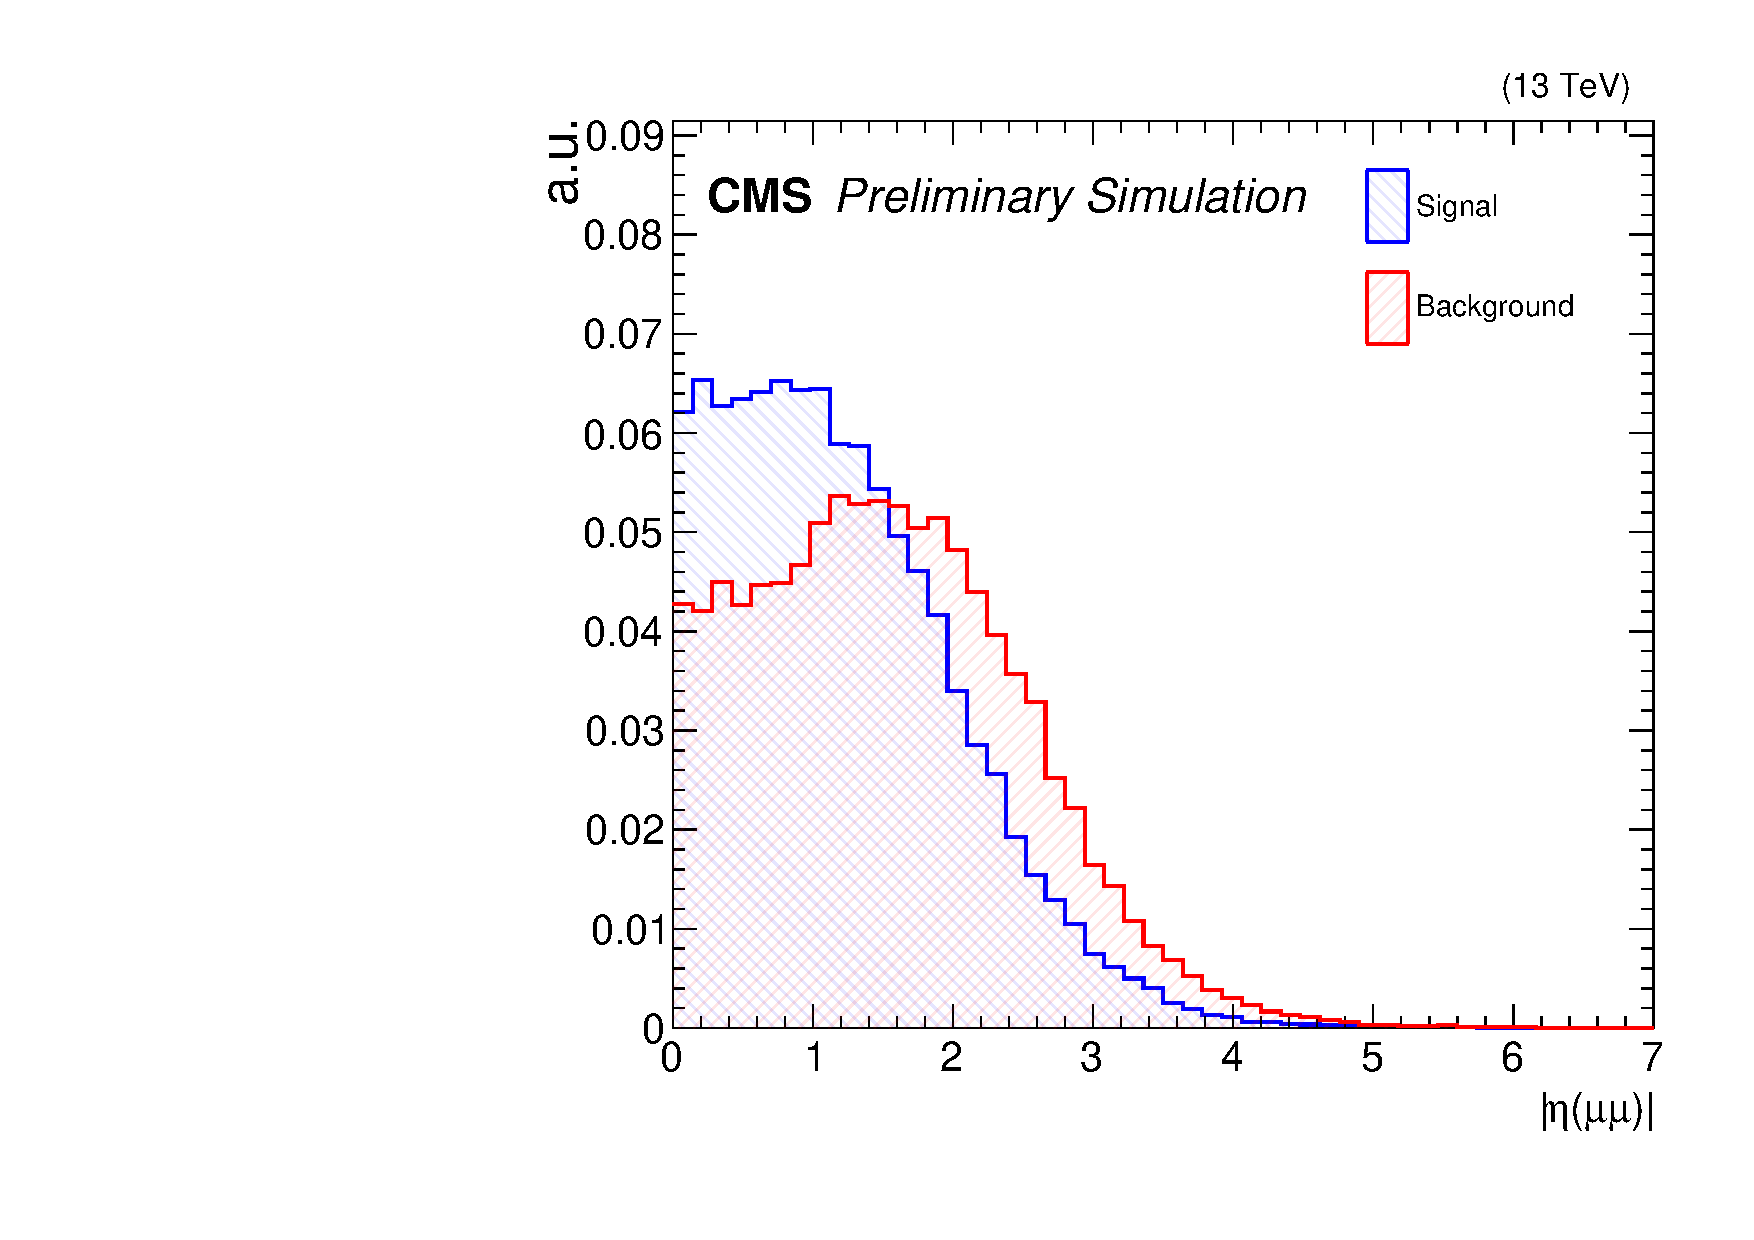
\includegraphics[width=0.24\textwidth]{pics/VH_sec/BDT_train_ZH/BDT_dimu_abs_eta.pdf}
    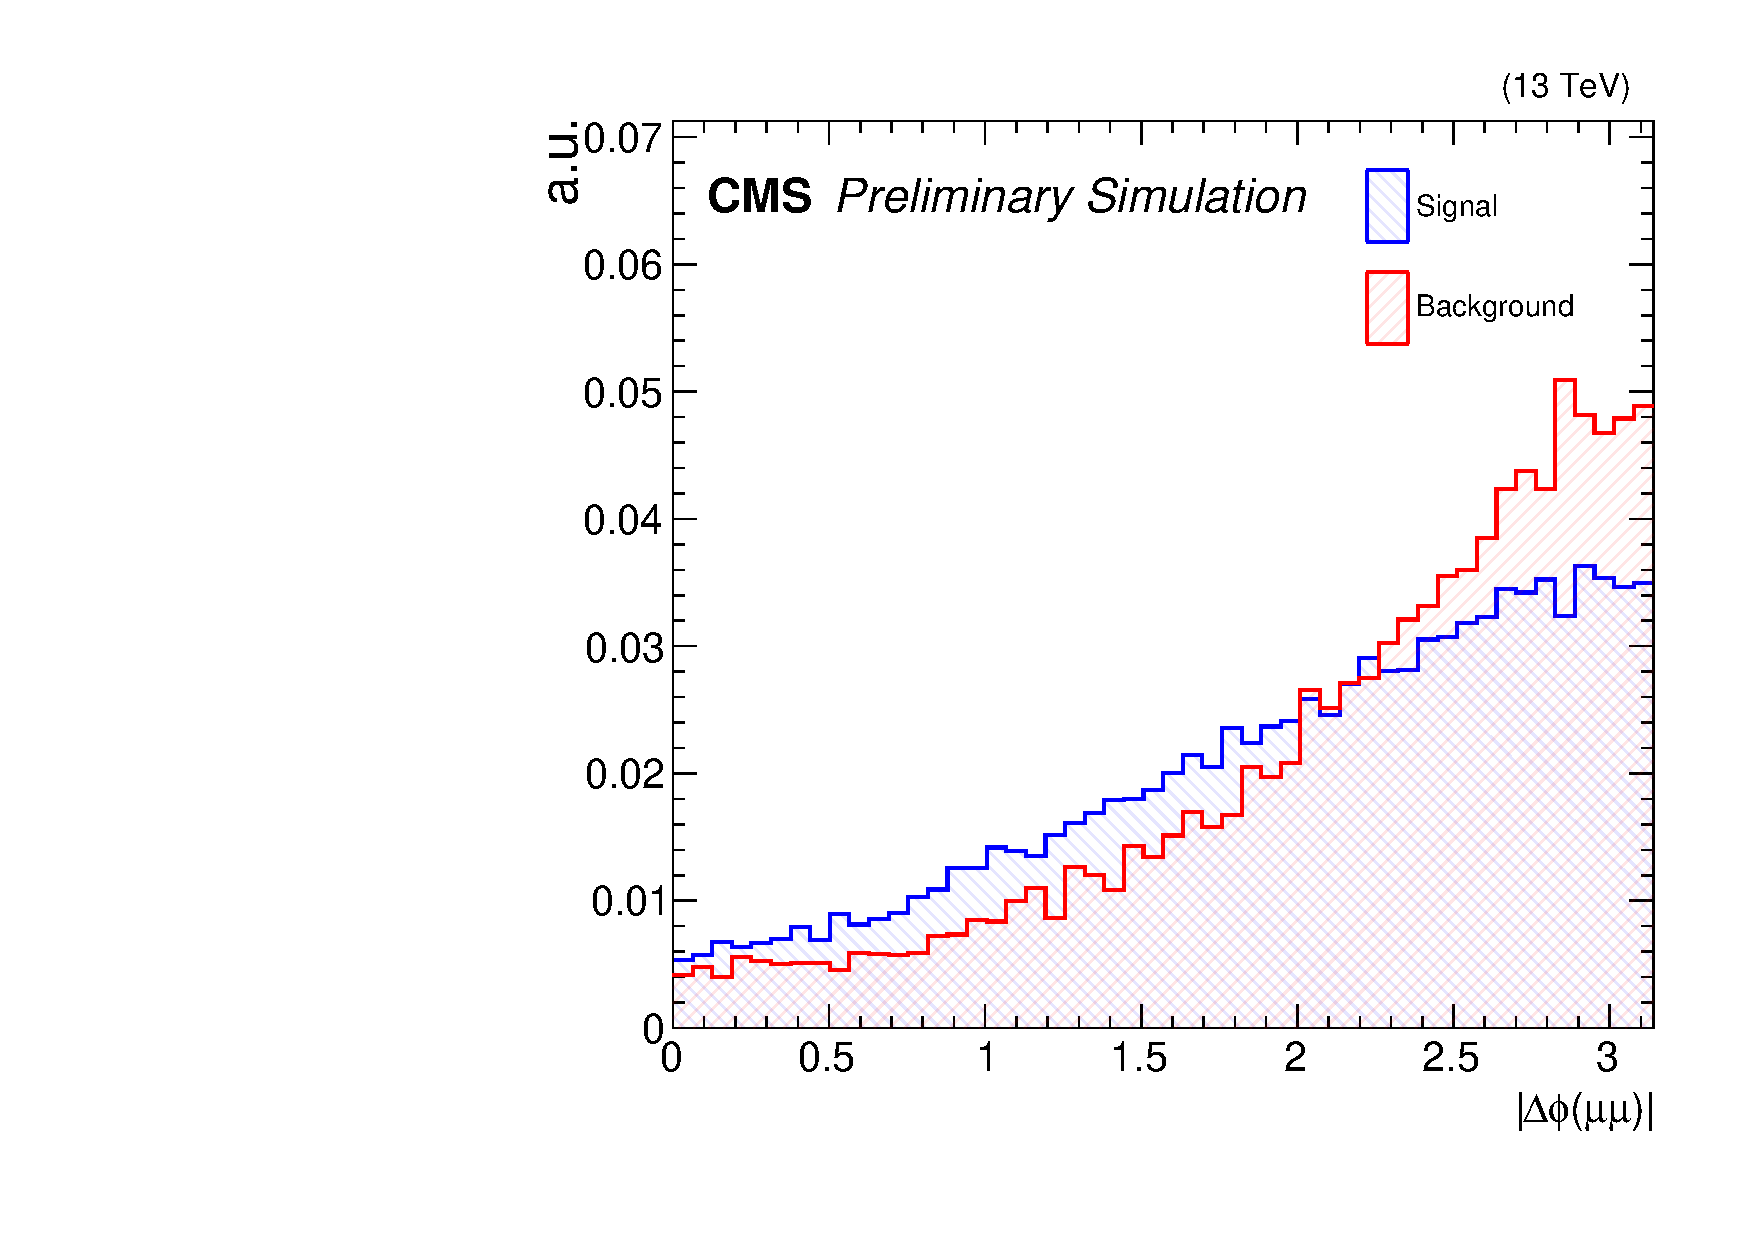
\includegraphics[width=0.24\textwidth]{pics/VH_sec/BDT_train_ZH/BDT_dimu_abs_dPhi.pdf}           
    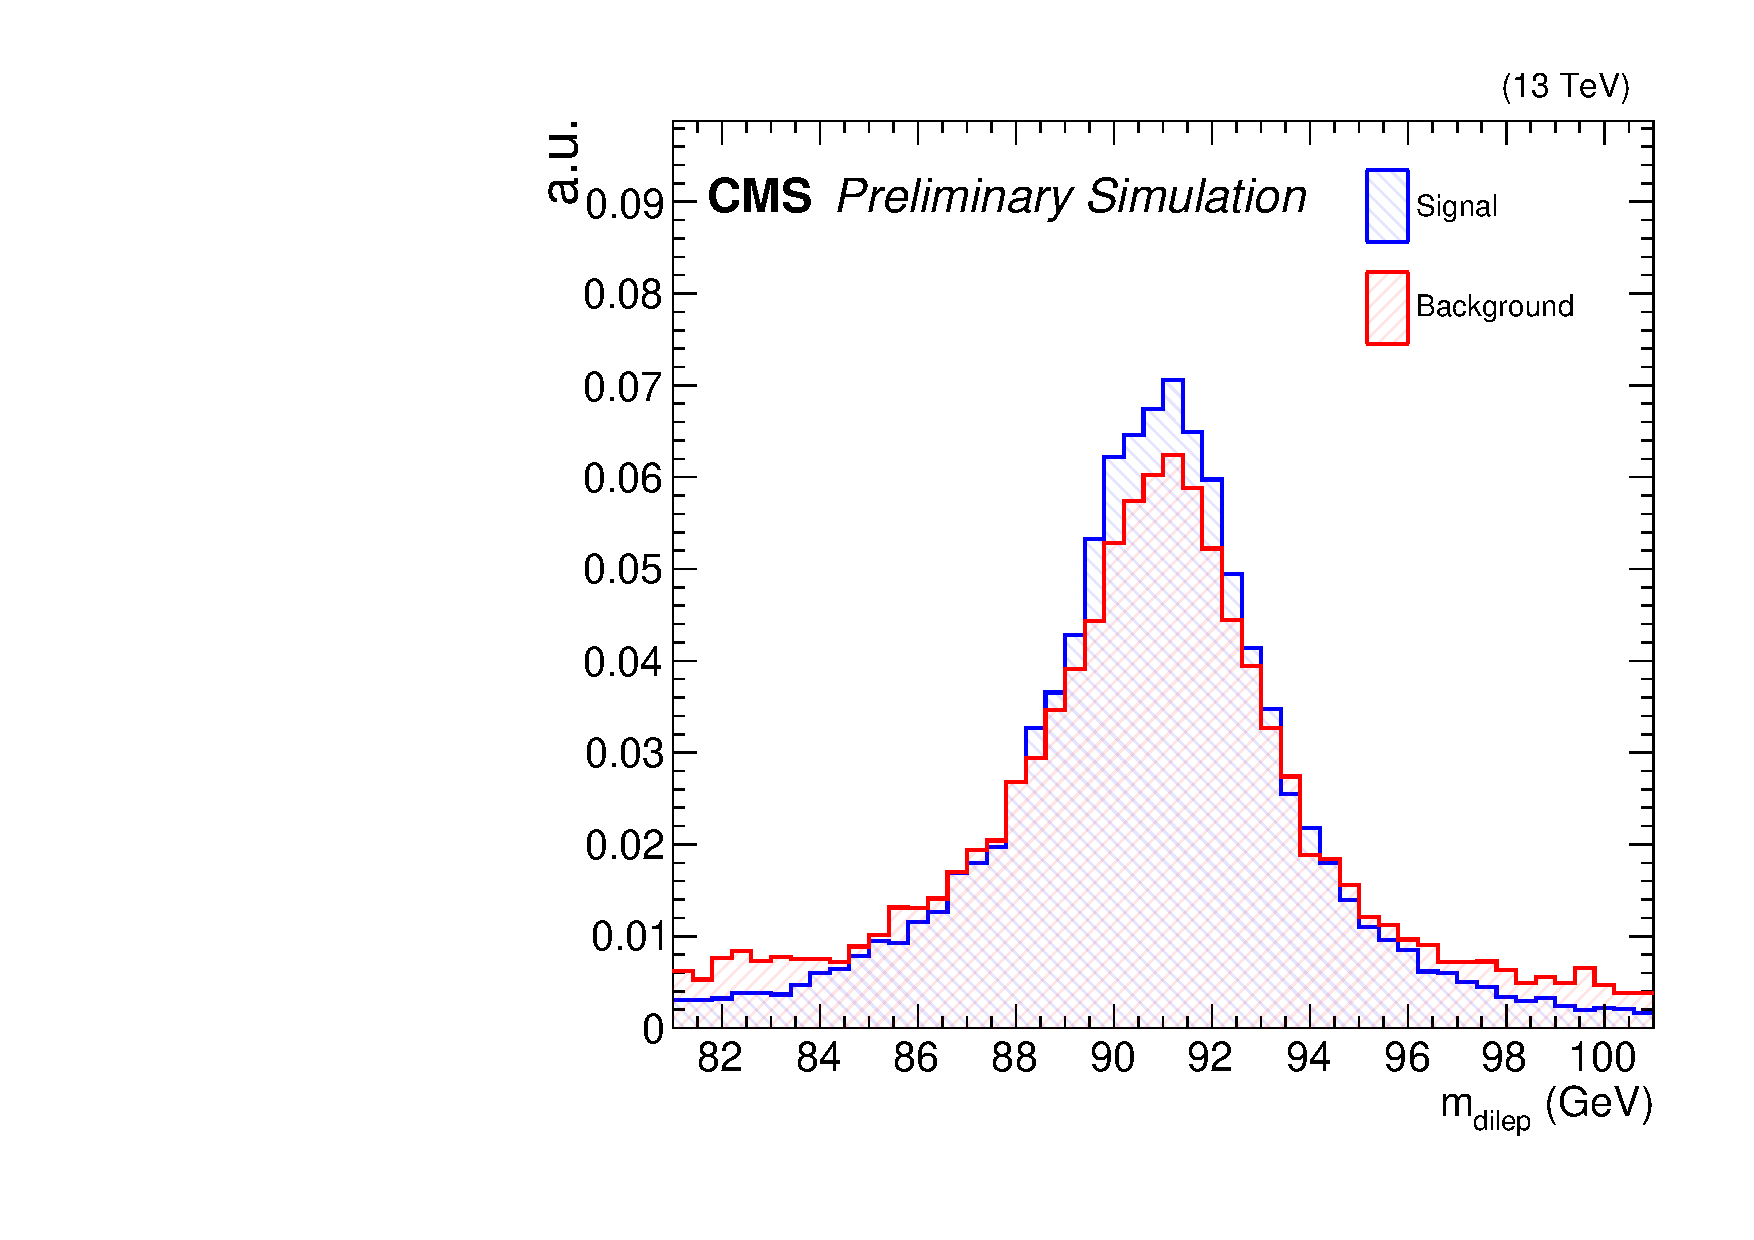
\includegraphics[width=0.24\textwidth]{pics/VH_sec/BDT_train_ZH/BDT_dilep_mass.pdf}

    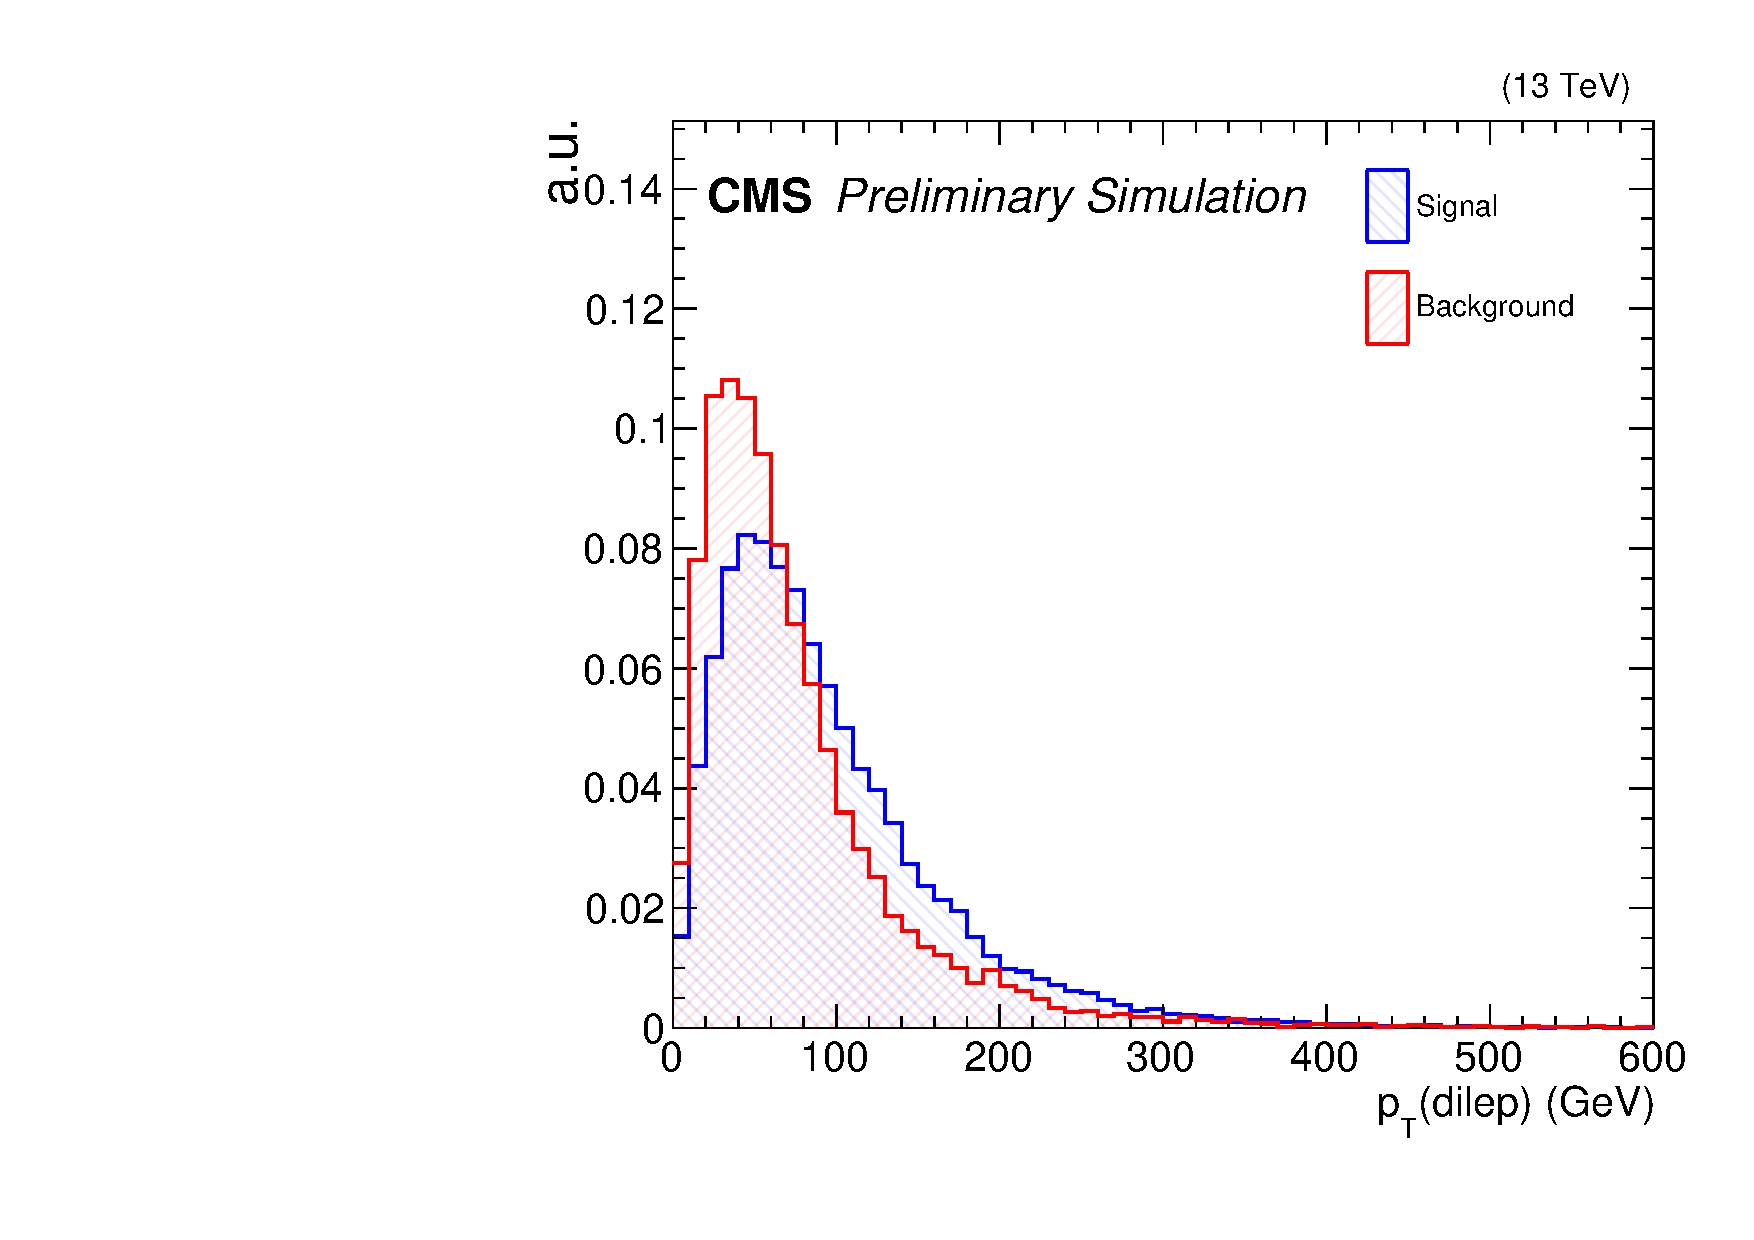
\includegraphics[width=0.24\textwidth]{pics/VH_sec/BDT_train_ZH/BDT_dilep_pt.pdf}           
    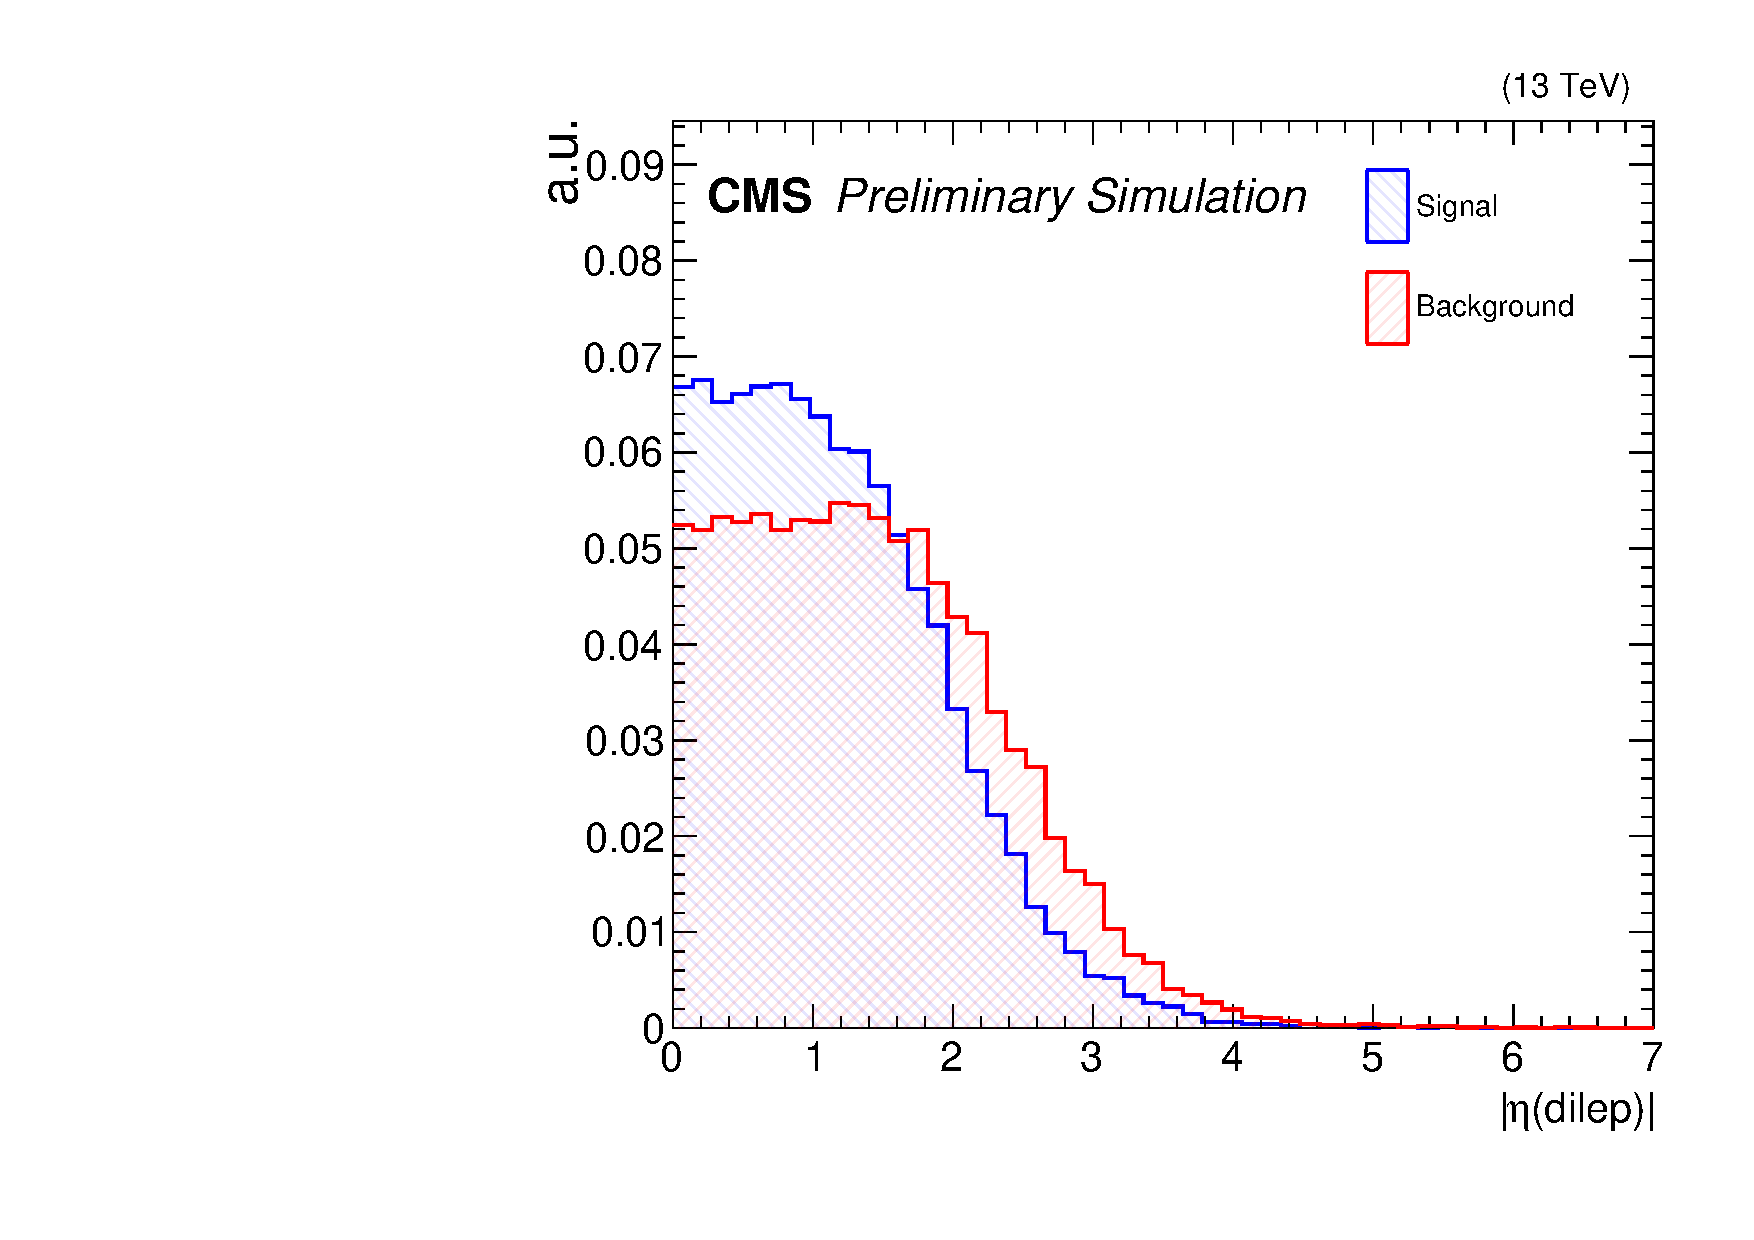
\includegraphics[width=0.24\textwidth]{pics/VH_sec/BDT_train_ZH/BDT_dilep_abs_eta.pdf}
    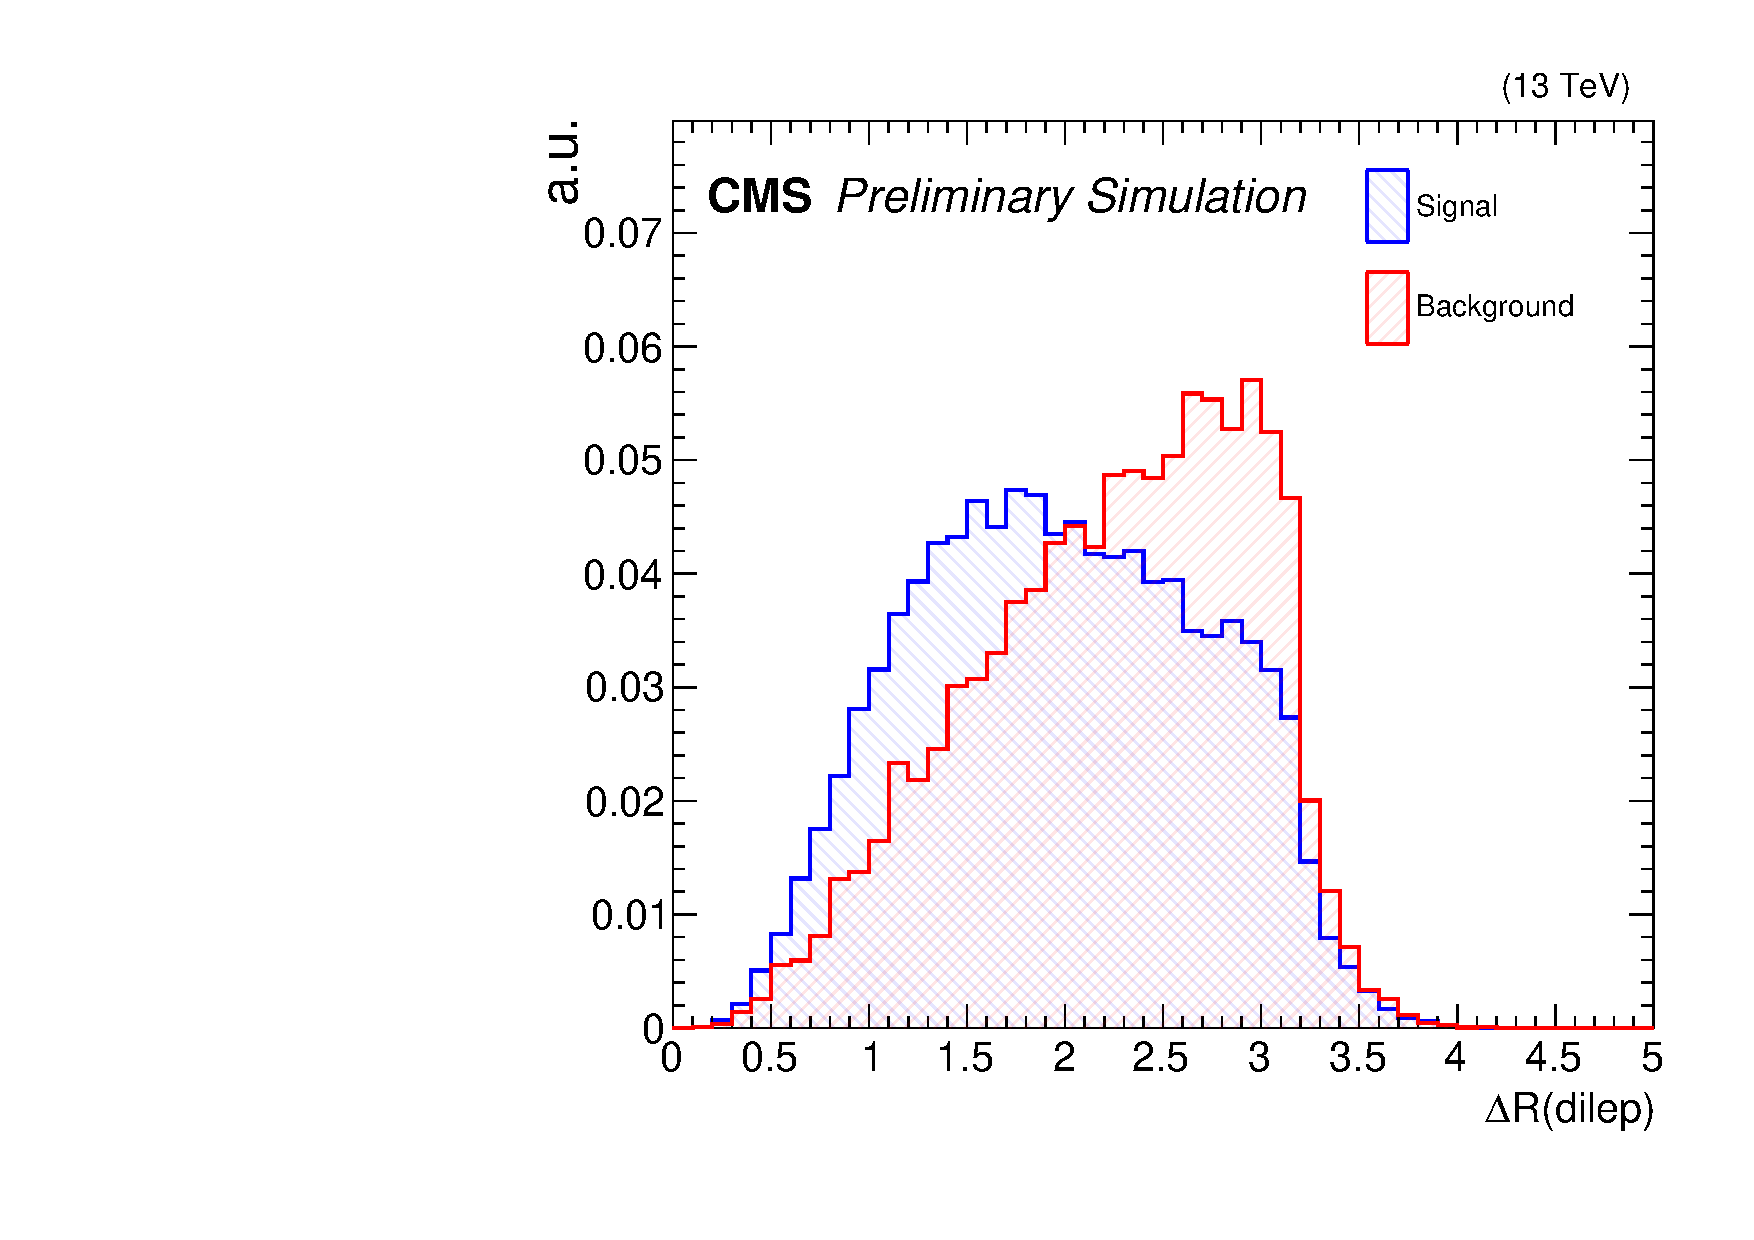
\includegraphics[width=0.24\textwidth]{pics/VH_sec/BDT_train_ZH/BDT_dilep_dR.pdf}           
    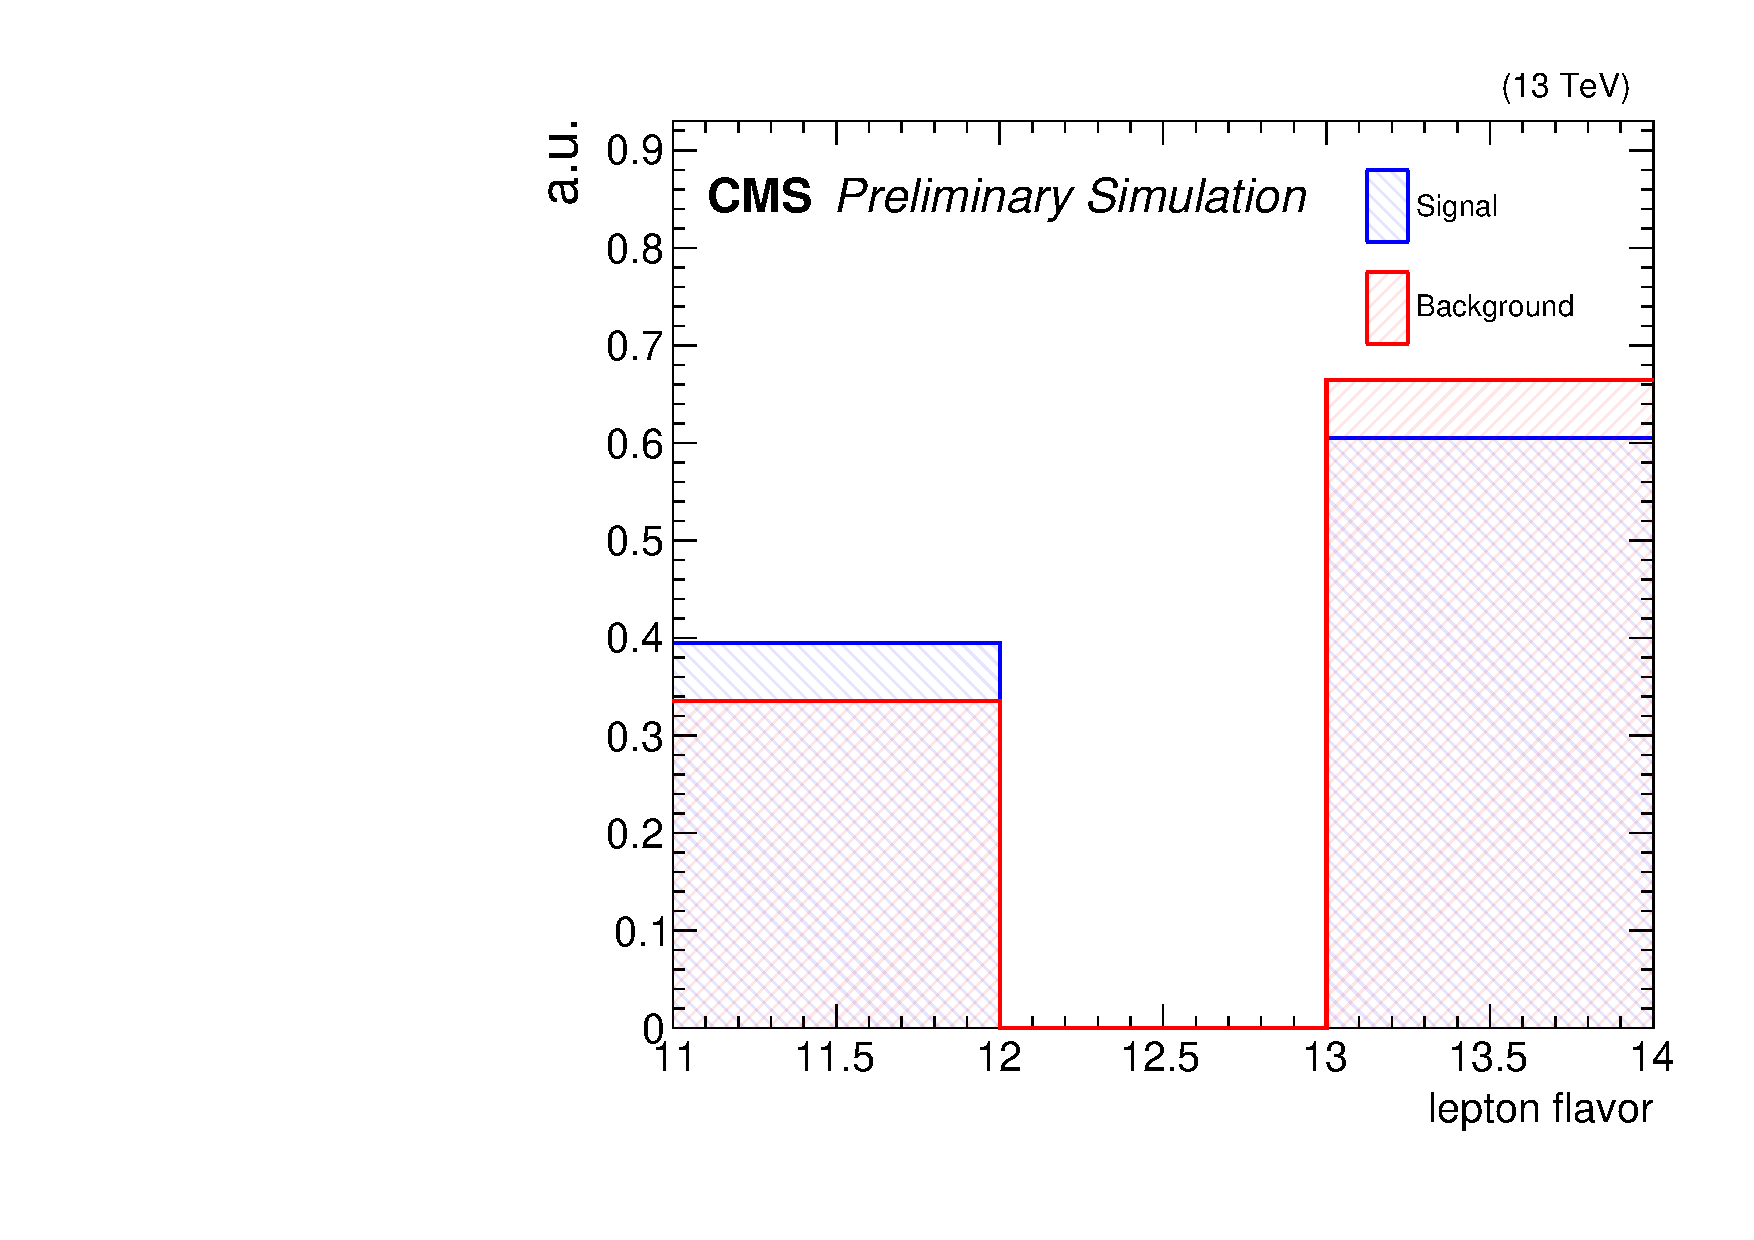
\includegraphics[width=0.24\textwidth]{pics/VH_sec/BDT_train_ZH/BDT_lep_ID.pdf}

    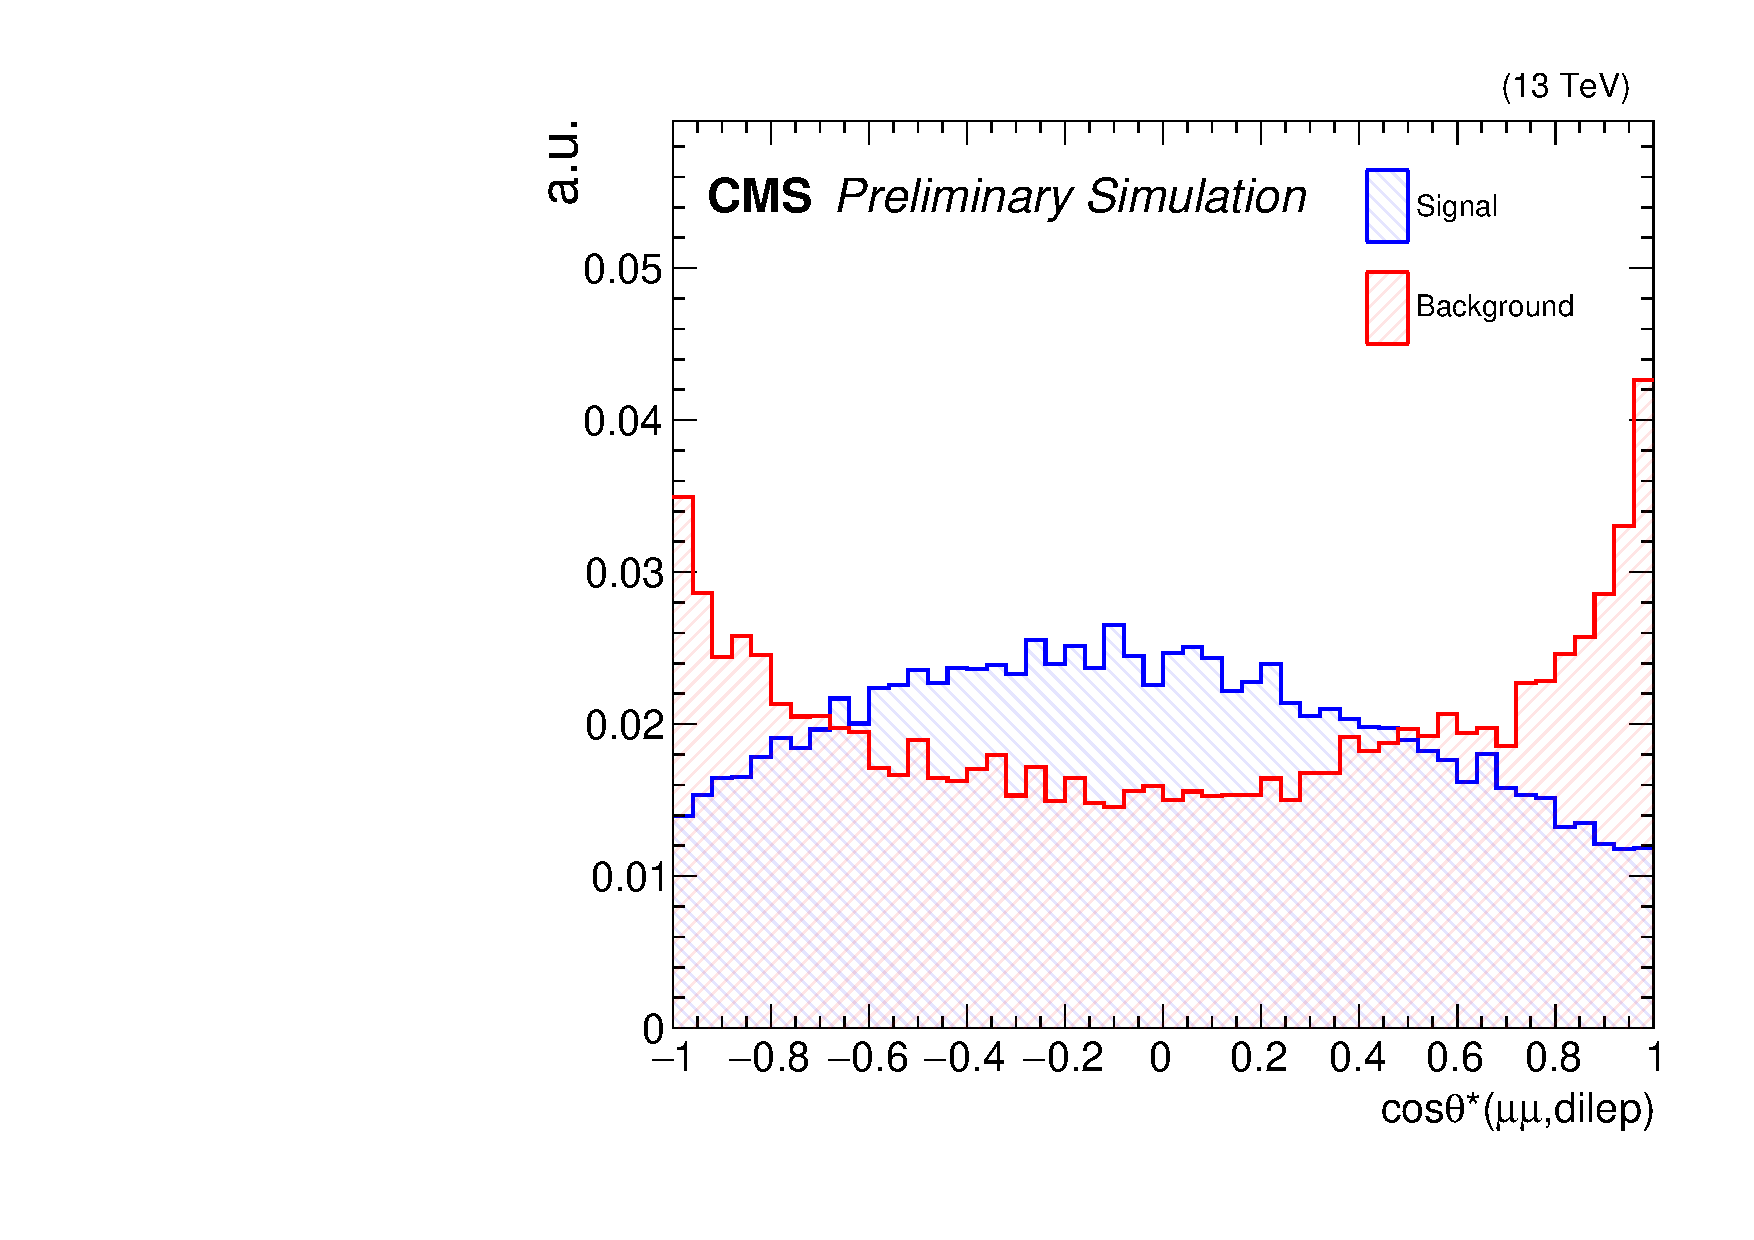
\includegraphics[width=0.24\textwidth]{pics/VH_sec/BDT_train_ZH/BDT_cts_dipair_H.pdf}           
    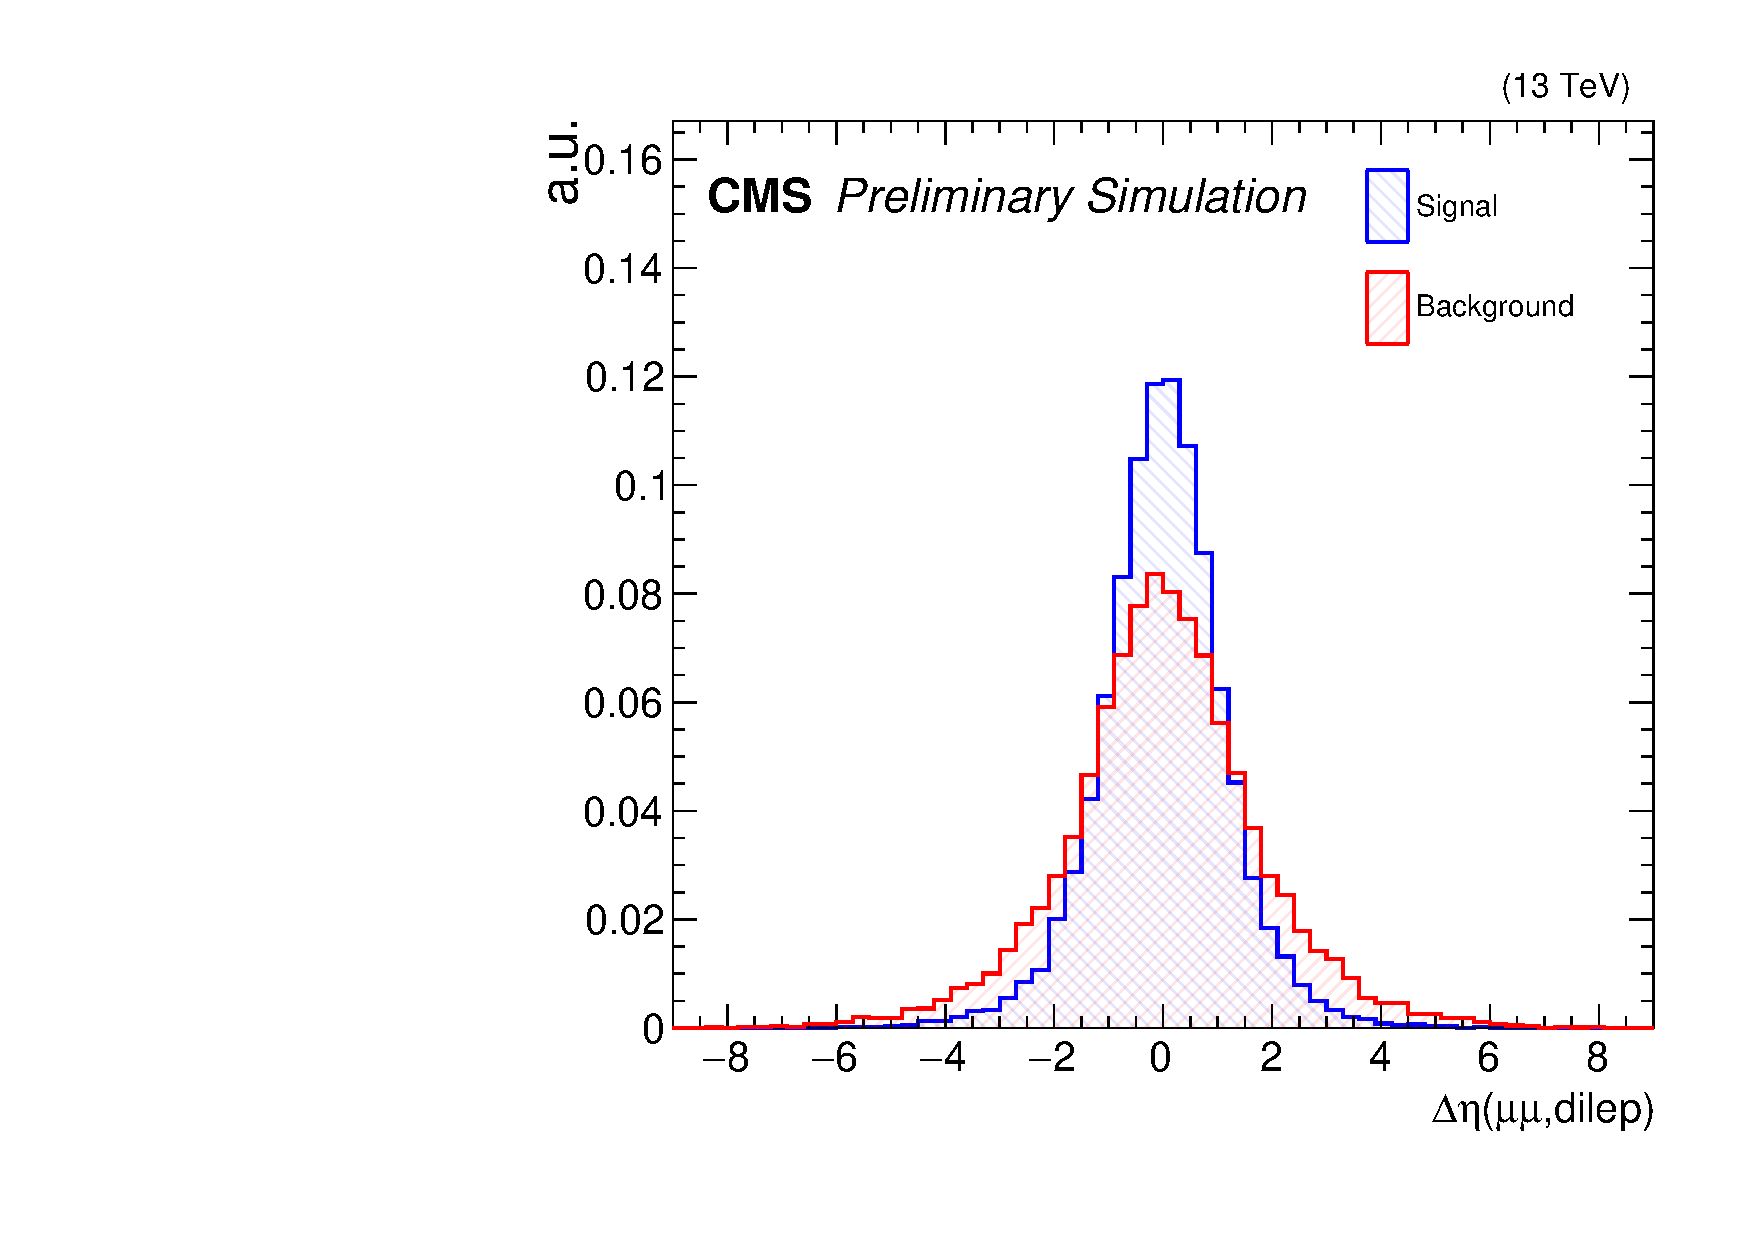
\includegraphics[width=0.24\textwidth]{pics/VH_sec/BDT_train_ZH/BDT_dipair_dEta_H.pdf}

    \caption{Input variables to the ZH $\to 4\ell$ BDT, with signal in blue and background in red.}
    \label{fig:zh_bdt_vars}
\end{figure*}


\clearpage
\subsection{Validation of the BDTs}\label{subsec:bdt_validation}

As discussed in~\ref{sec:hmm_cat_and_strategy}, the strategy of this analysis is to divide events into subcategories with different \SoB,
and consequently maximize the overall sensitivity.
The signal extraction is performed by fitting the \mmm spectrum, therefore it is crucial that 
any selection cut applied to the BDT score should not sculpt the \mmm shape.
Two checks are performed for this purpose:
\begin{itemize}
	\item The \mmm shape of the background is compared between events in different BDT quantiles, shown as the left plots of Figures~\ref{fig:wh_bdt_mass} and~\ref{fig:zh_bdt_mass}. 
	\item The BDT output is compared between several signal samples with different \mh assumptions, shown as the right plots of Figures~\ref{fig:wh_bdt_mass} and~\ref{fig:zh_bdt_mass}.
\end{itemize}
The \mmm shape of the background in all BDT quantiles are smooth falling.
The left plot of Figure~\ref{fig:wh_bdt_mass} shows a mild dependence of slope on the BDT quantiles.
But no spurious peak-like structure is seen in any of the distributions.
This slope difference should not affect the signal evaluation.
The BDT distributions in different signal samples agree very well,
so the BDTs are not biased toward any particular \mmm range. 
Overall, the \WH and \ZH BDTs do not sculpt of the \mmm shape
and can be used for categorization.

\begin{figure*}[!htb]
  \centering
  \captionsetup{justification=justified}
  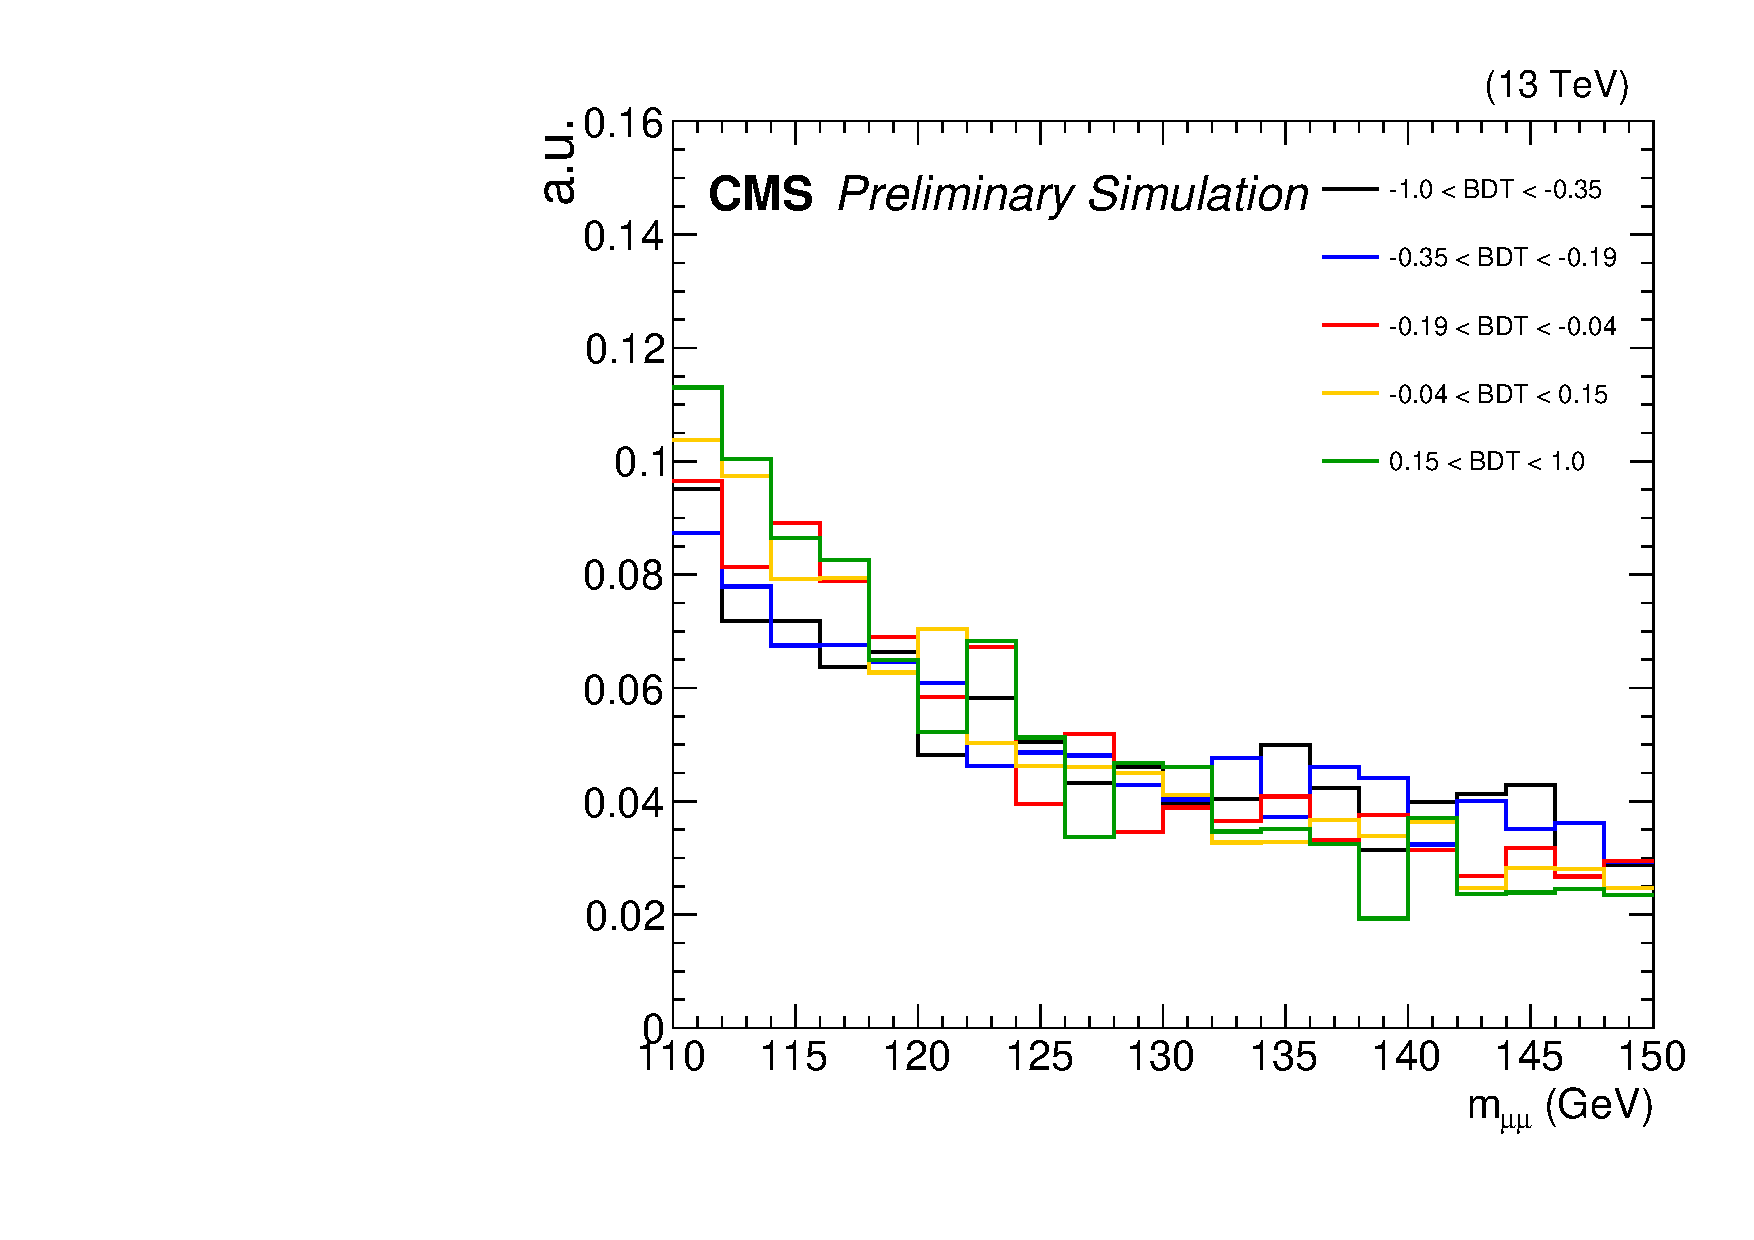
\includegraphics[width=0.42\textwidth]{pics/VH_sec/valid_BDT_WH/mass_in_WH_BDT_quantiles.pdf}
  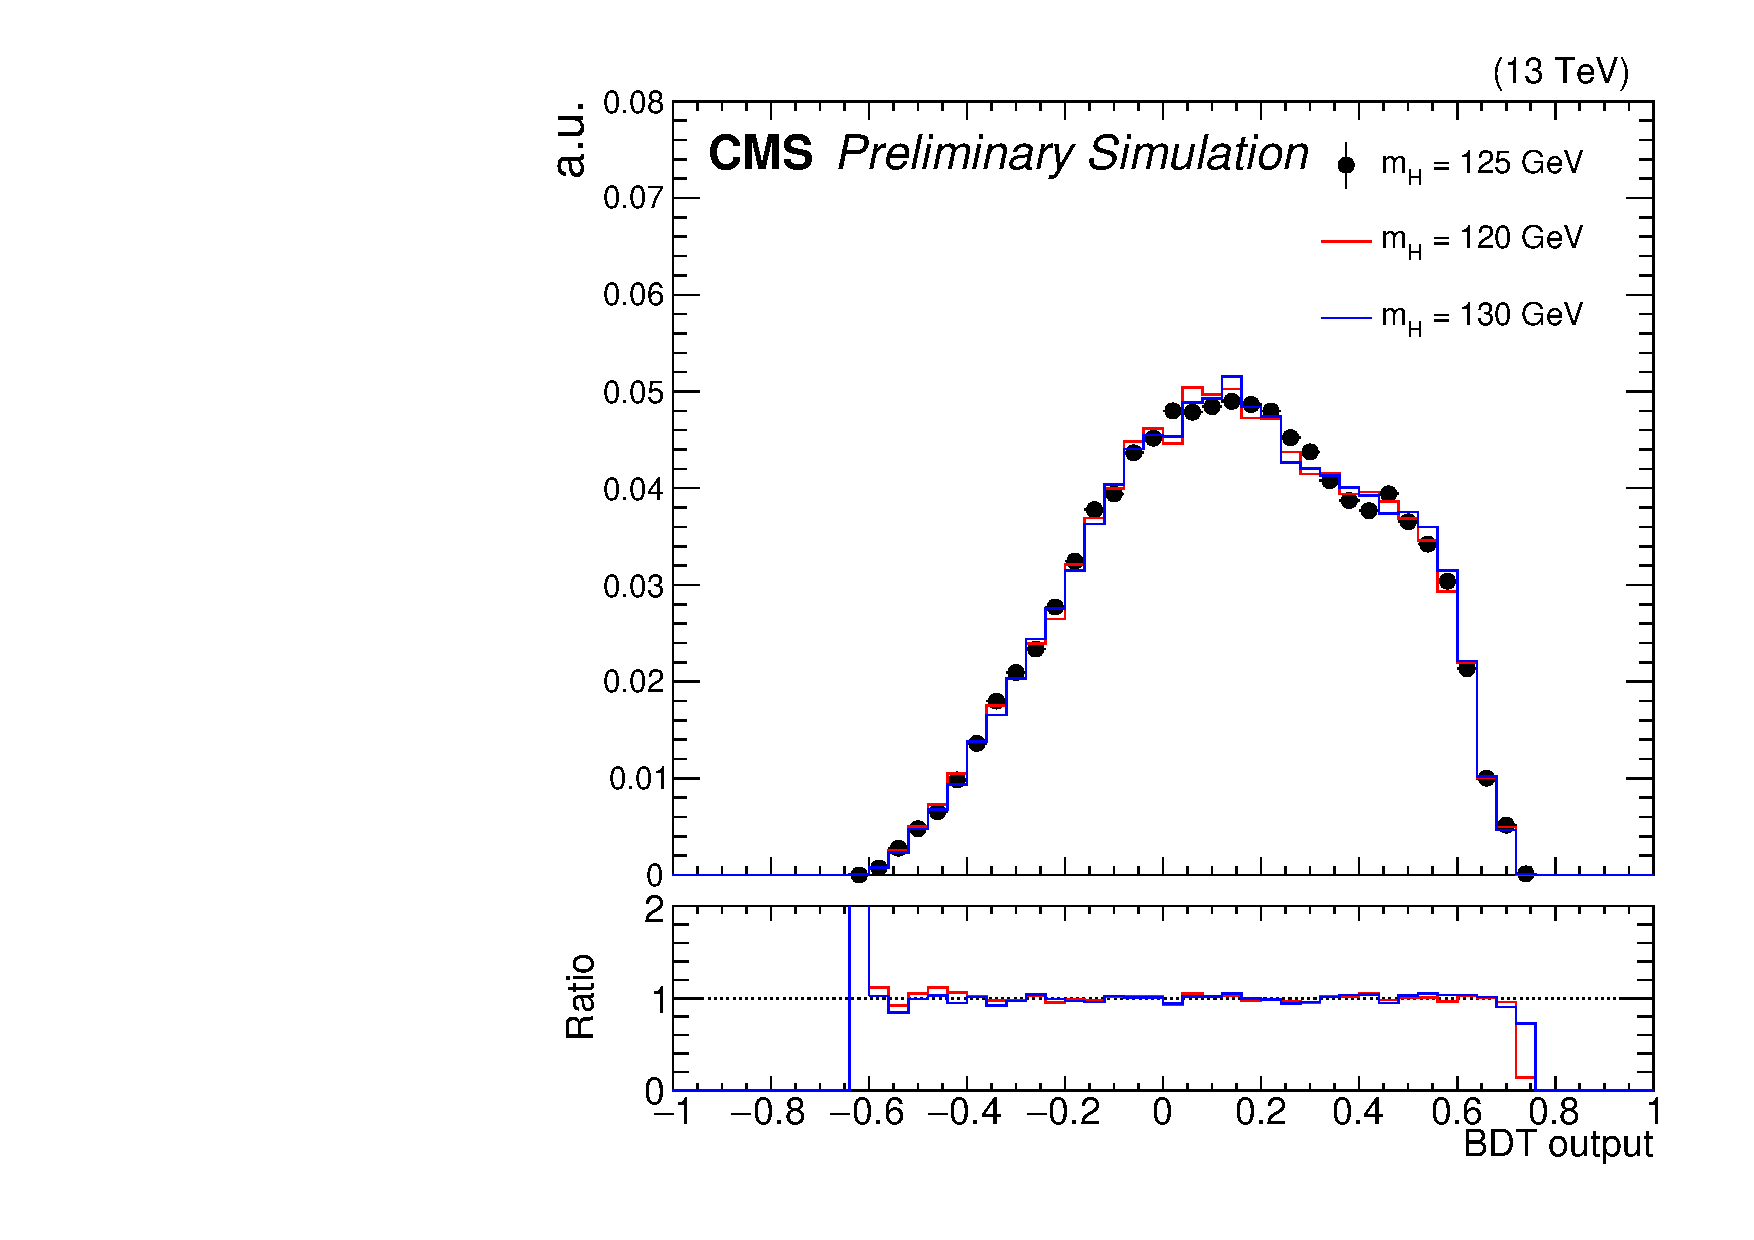
\includegraphics[width=0.42\textwidth]{pics/VH_sec/valid_BDT_WH/WH_BDT_three_sigs.pdf}
  \caption{For the WH BDT, the distribution of the dimuon mass shape in the background for five different BDT quantile (left), 
           and the distribution of the BDT output for three different signal mass assumptions (right).}
  \label{fig:wh_bdt_mass}
\end{figure*}

\begin{figure*}[!htb]
  \centering
  \captionsetup{justification=justified}
  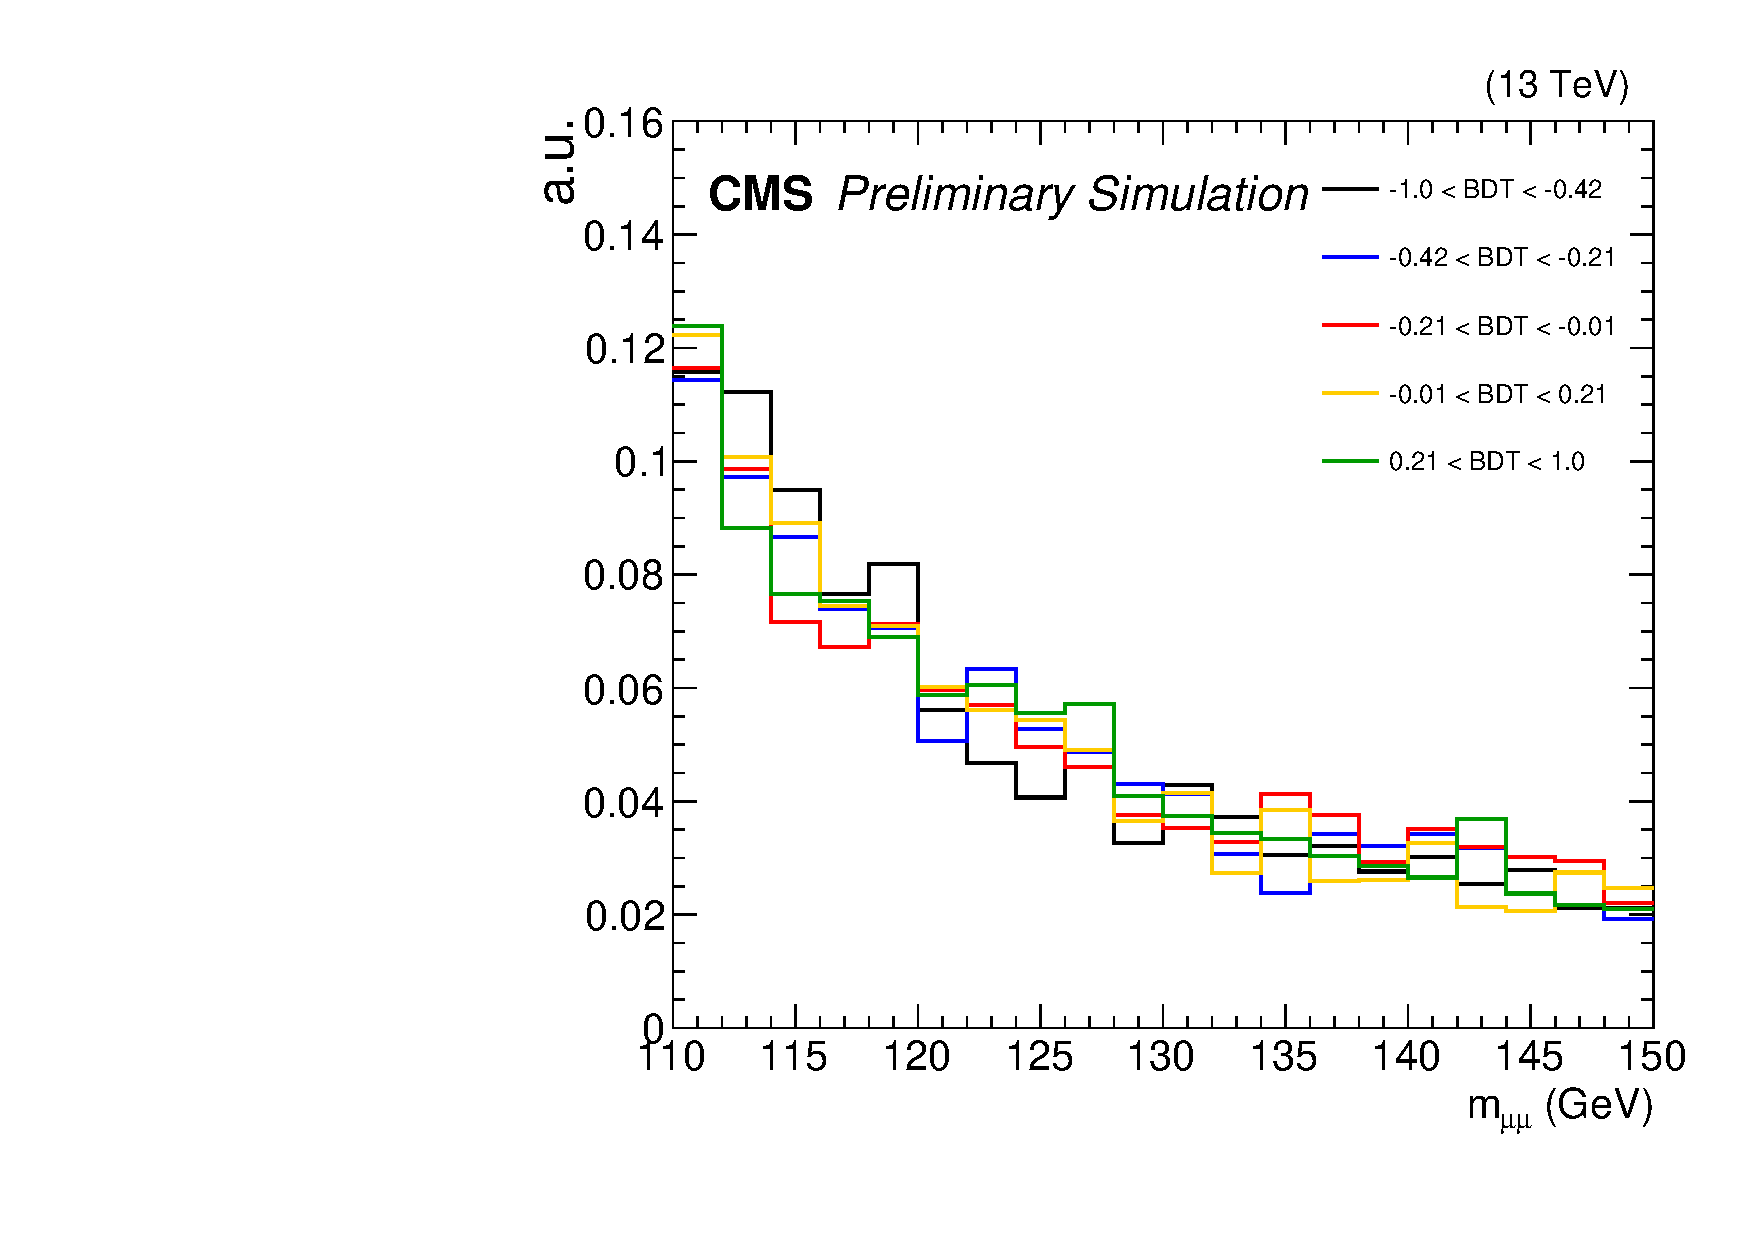
\includegraphics[width=0.42\textwidth]{pics/VH_sec/valid_BDT_ZH/mass_in_ZH_BDT_quantiles.pdf}
  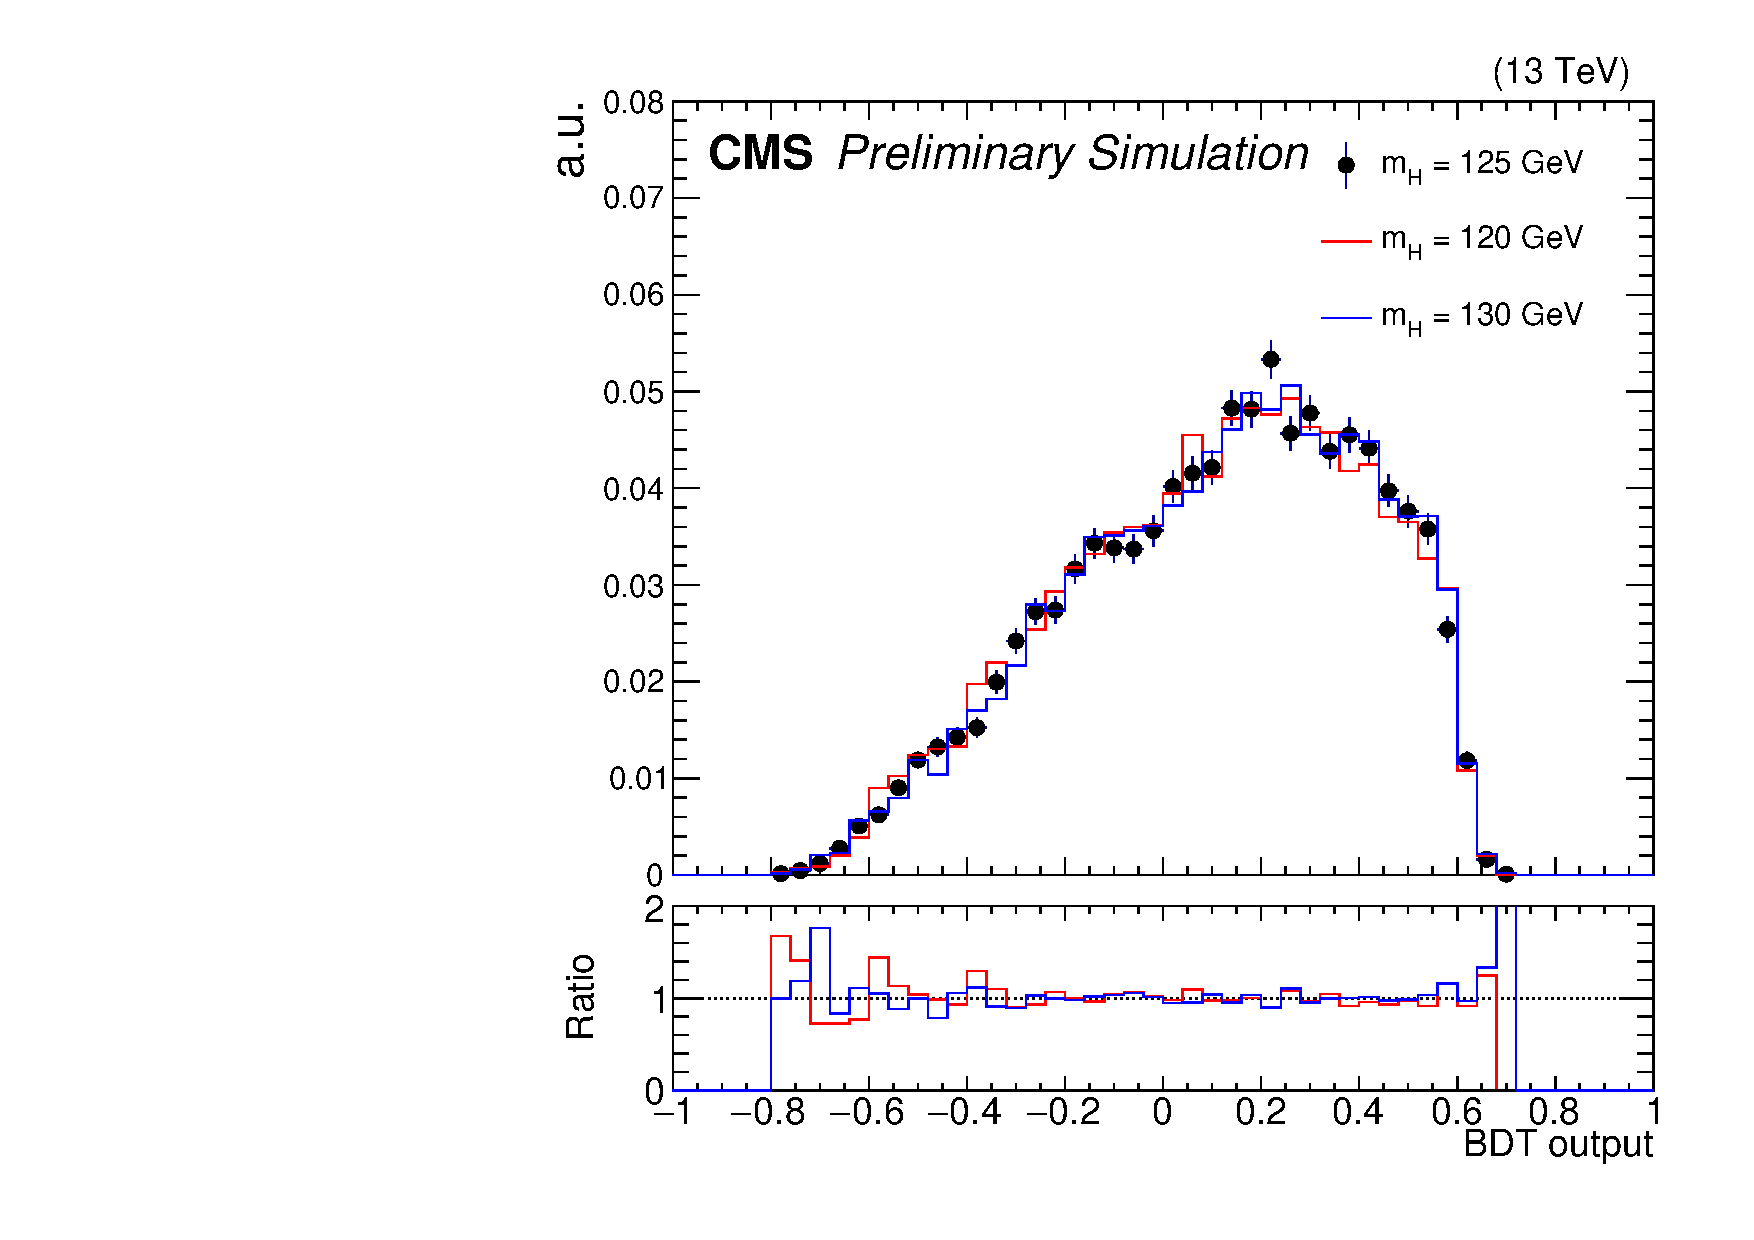
\includegraphics[width=0.42\textwidth]{pics/VH_sec/valid_BDT_ZH/ZH_BDT_three_sigs.pdf}
  \caption{For the \ZH BDT, the distribution of the dimuon mass shape in the background for five different BDT quantile (left),
           and the distribution of the BDT output for three different signal mass assumptions (right).}
  \label{fig:zh_bdt_mass}
\end{figure*}


Furthermore, it is also important to make sure the BDT would perform the same way on data as it does on simulation.
In order to do this, the inputs and output of the BDTs are plotted comparing between data and the simulation.
Figure~\ref{fig:vh_bdt_output_data} shows the output of the \WH BDT and the \ZH BDT, 
and Figure~\ref{fig:wh_bdt_inputs_data} and~\ref{fig:zh_bdt_inputs_data} show the input variables to the \WH and \ZH BDTs respectively.
Overall, data and simulation agree with each other within the uncertainties for the BDT outputs and most of the inputs.
Some fluctuations are seen in data, especially in the \ZH category, as the total number of events is small. 
These fluctuations are expected within the statistical uncertainty and do not indicate any systematic disagreement.

\begin{figure*}[!htb]
  \centering
  \captionsetup{justification=justified}
  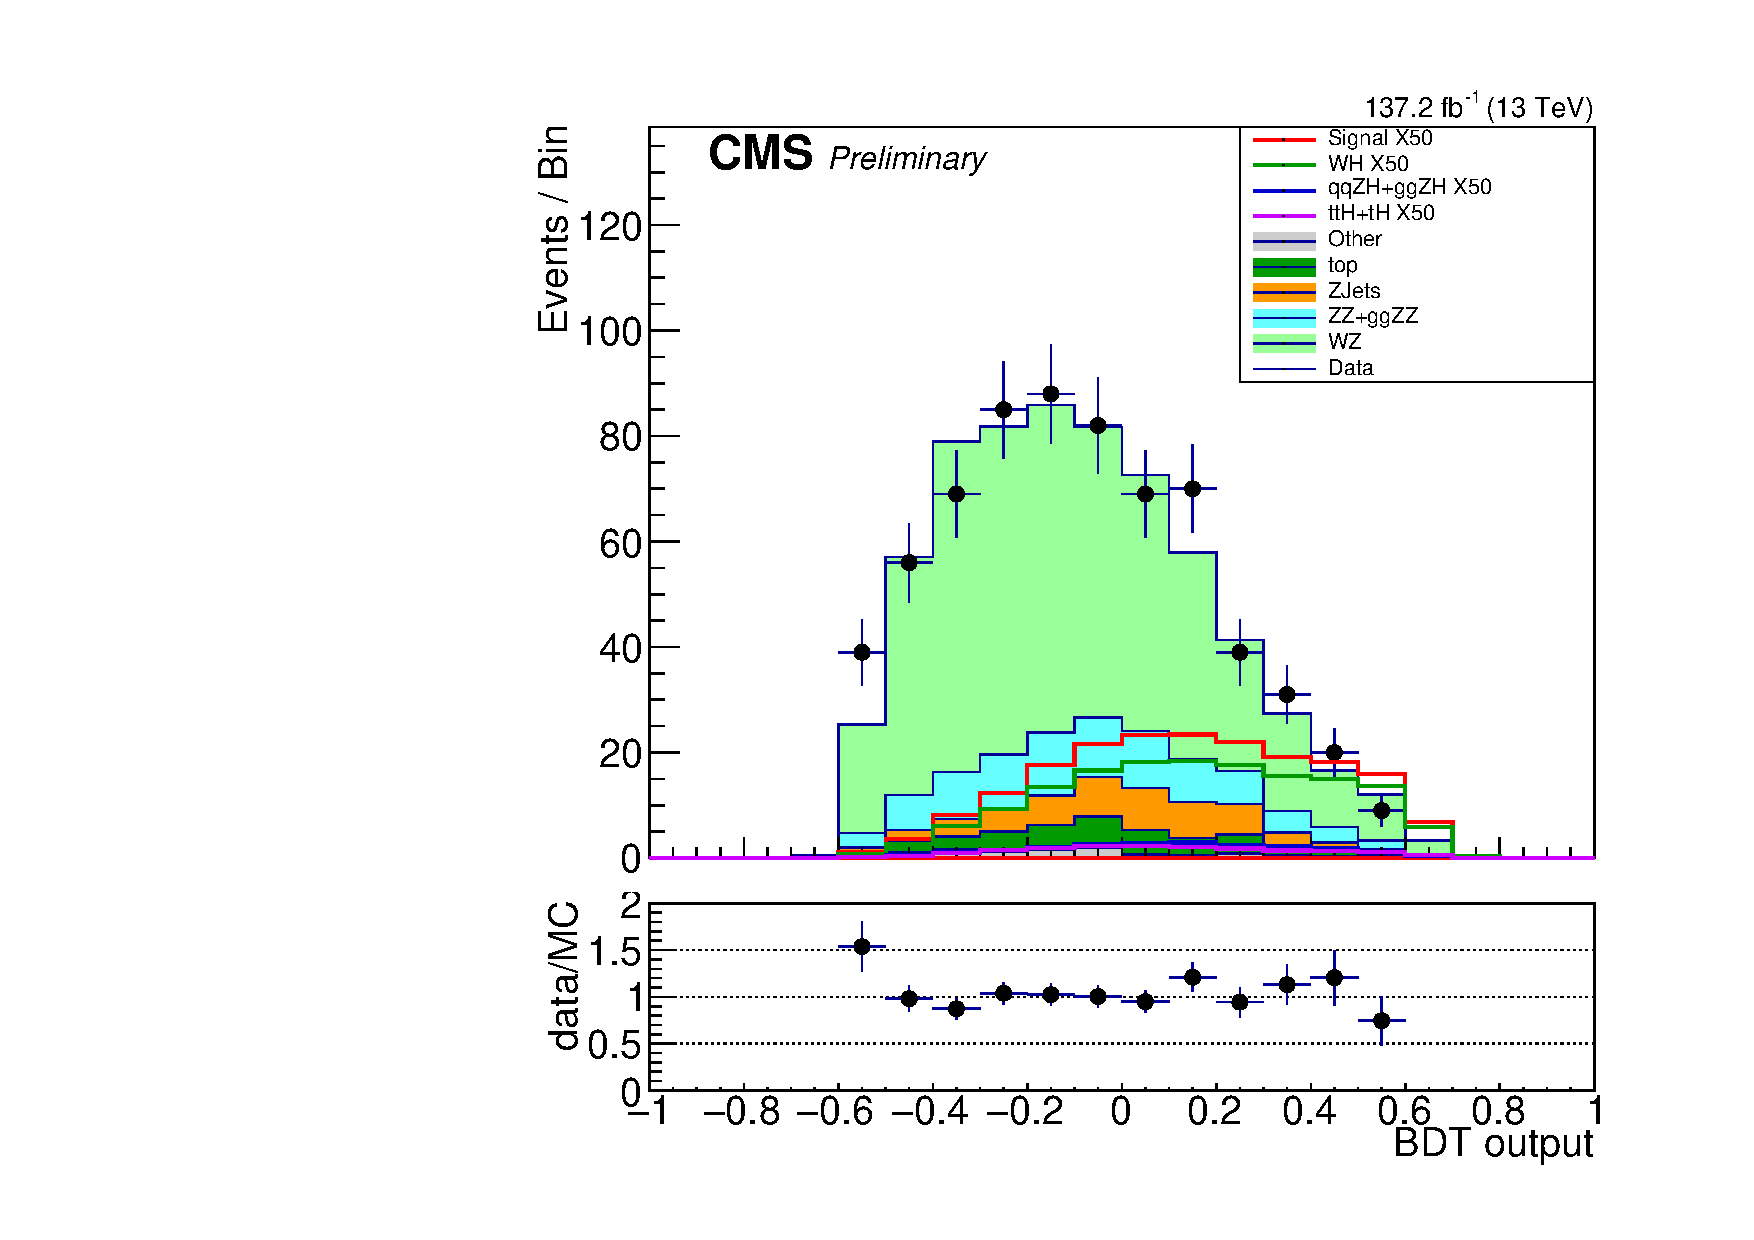
\includegraphics[width=0.42\textwidth]{pics/VH_sec/valid_BDT_WH/BDT_final.pdf}
  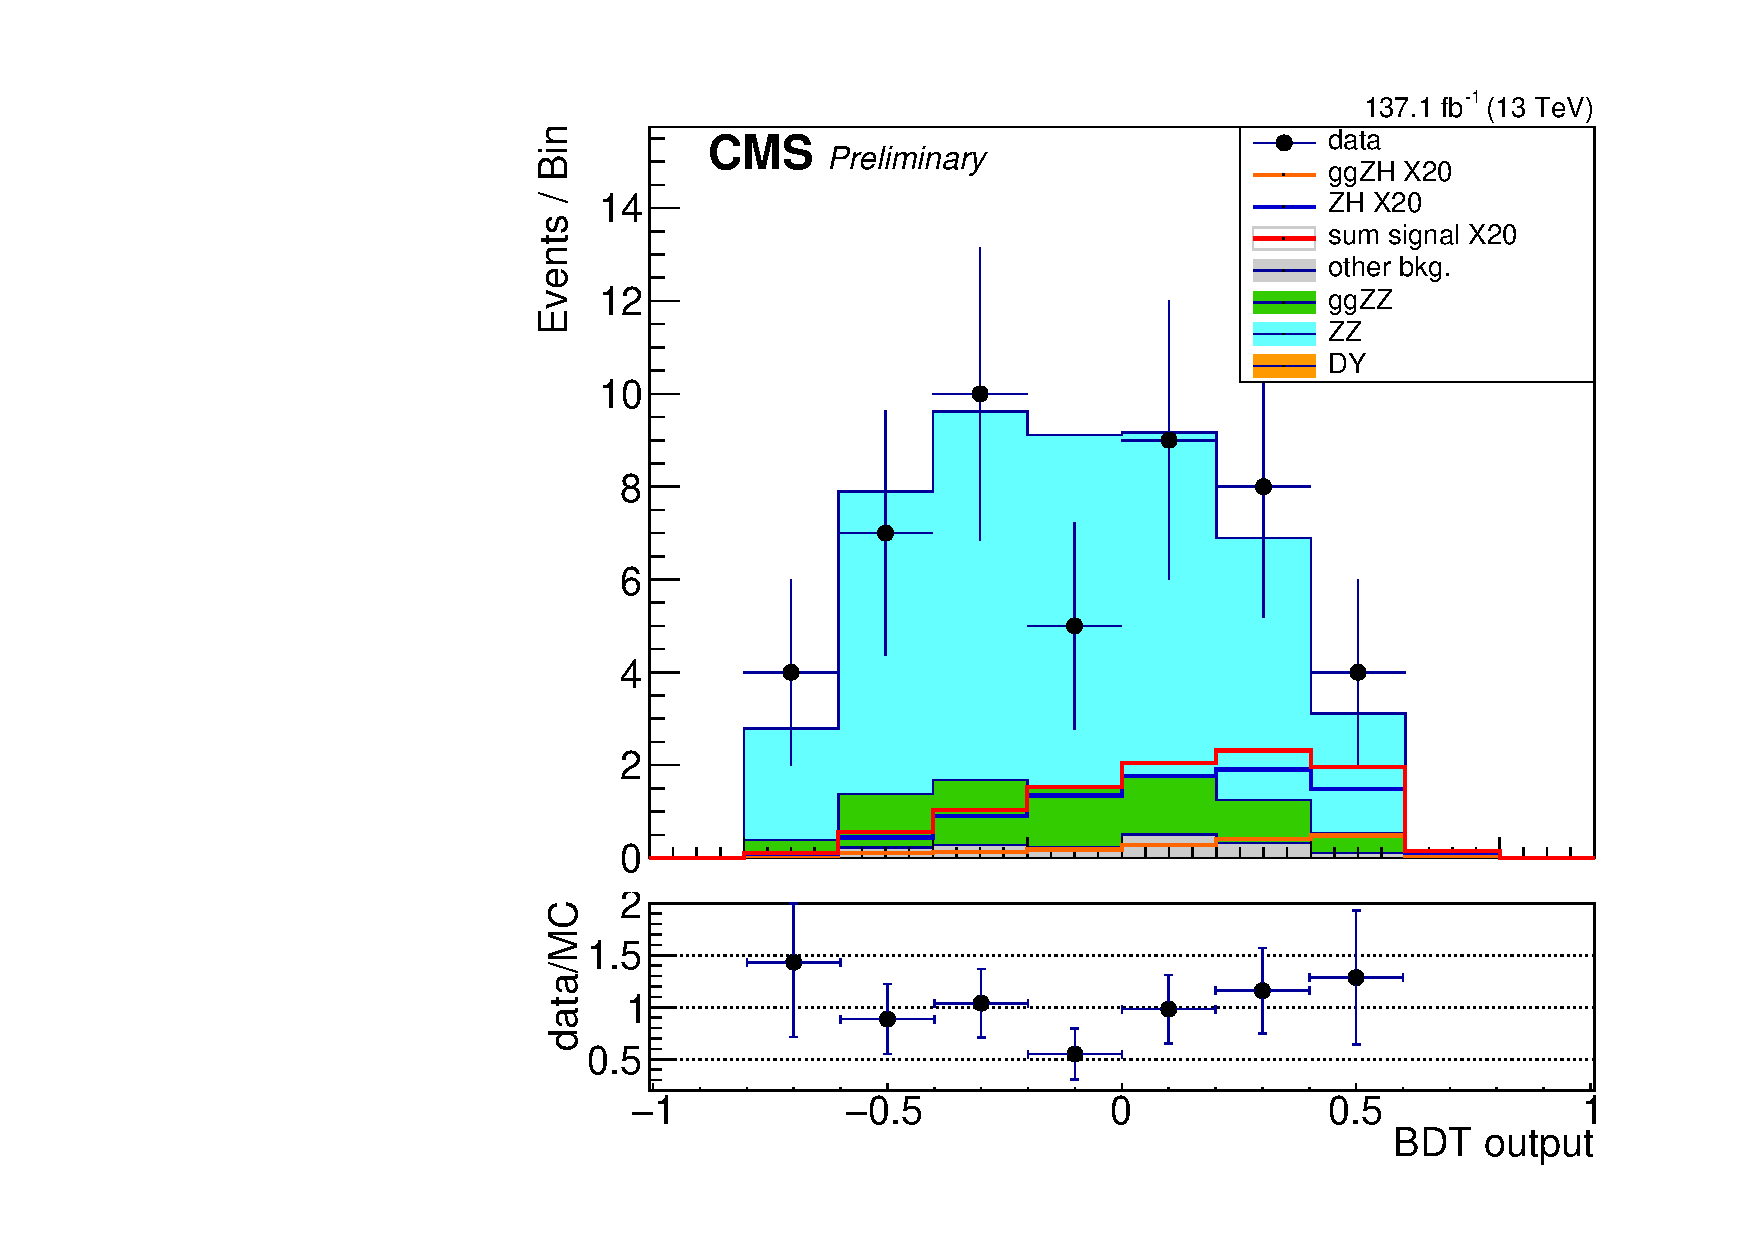
\includegraphics[width=0.42\textwidth]{pics/VH_sec/valid_BDT_ZH/BDT_final.pdf}
  \caption{The WH BDT output (left) and the \ZH BDT output (right) in full Run 2 in the signal region 110 \GeV $<$ \mmm $<$ 150 \GeV.}
  \label{fig:vh_bdt_output_data}
\end{figure*}

\begin{figure*}[!htb]
  \centering
  \captionsetup{justification=justified}
  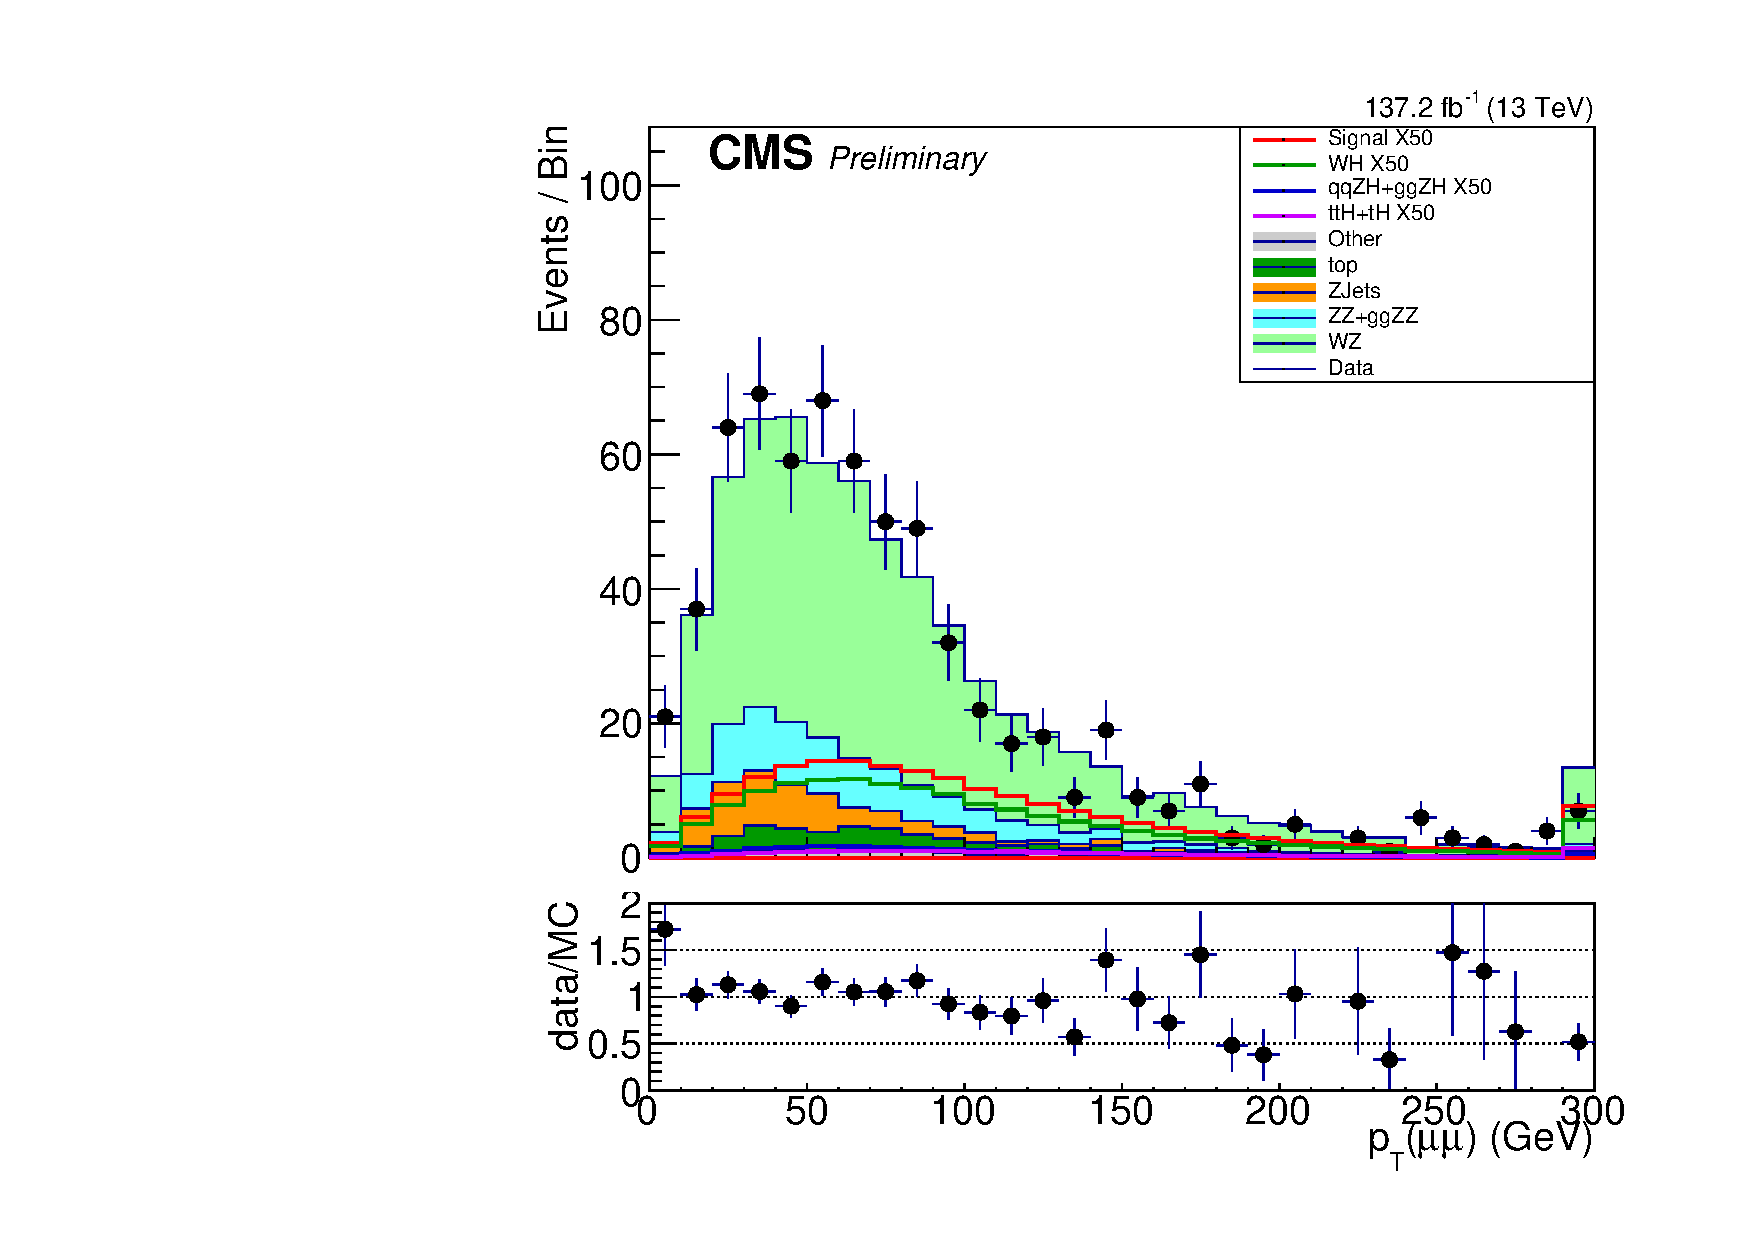
\includegraphics[width=0.24\textwidth]{pics/VH_sec/valid_BDT_WH/H_pair_pt.pdf}
  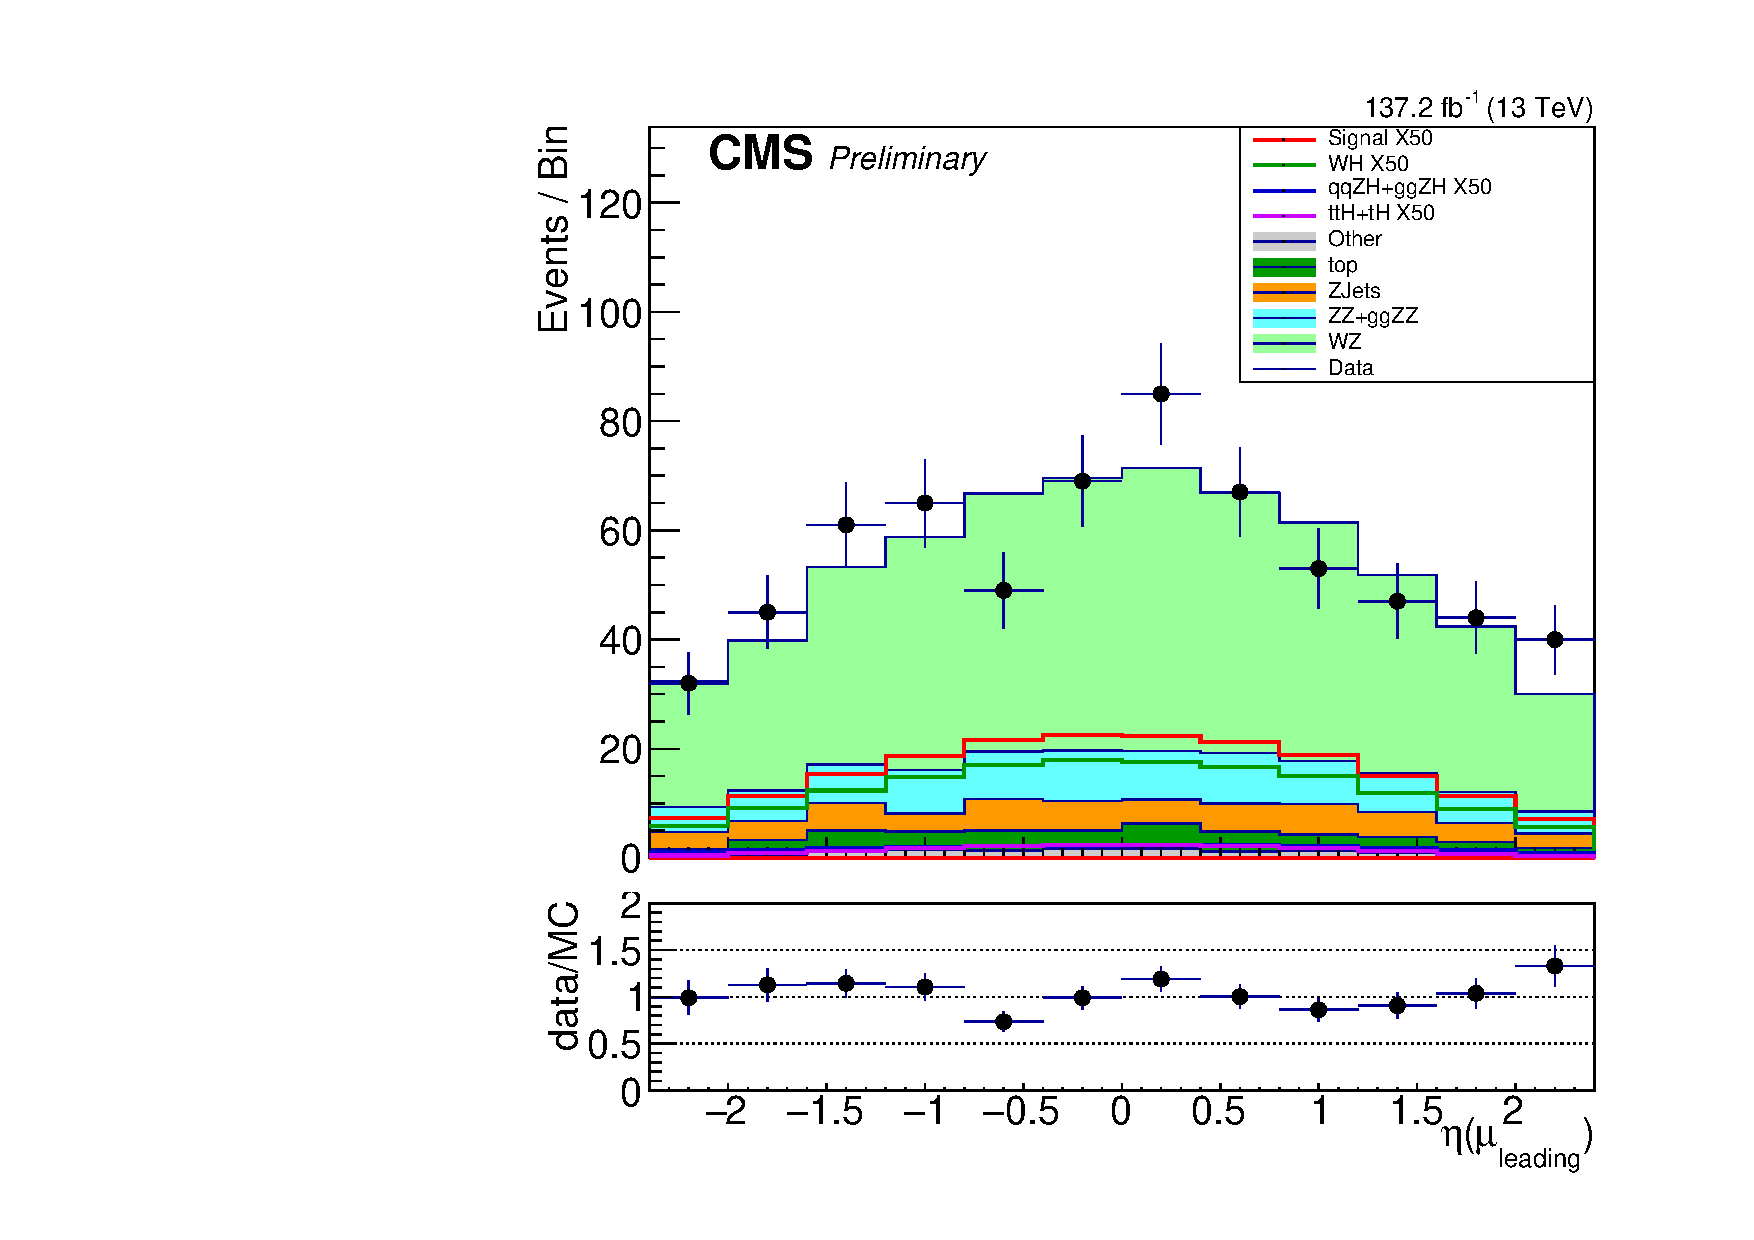
\includegraphics[width=0.24\textwidth]{pics/VH_sec/valid_BDT_WH/muH1_eta.pdf}
  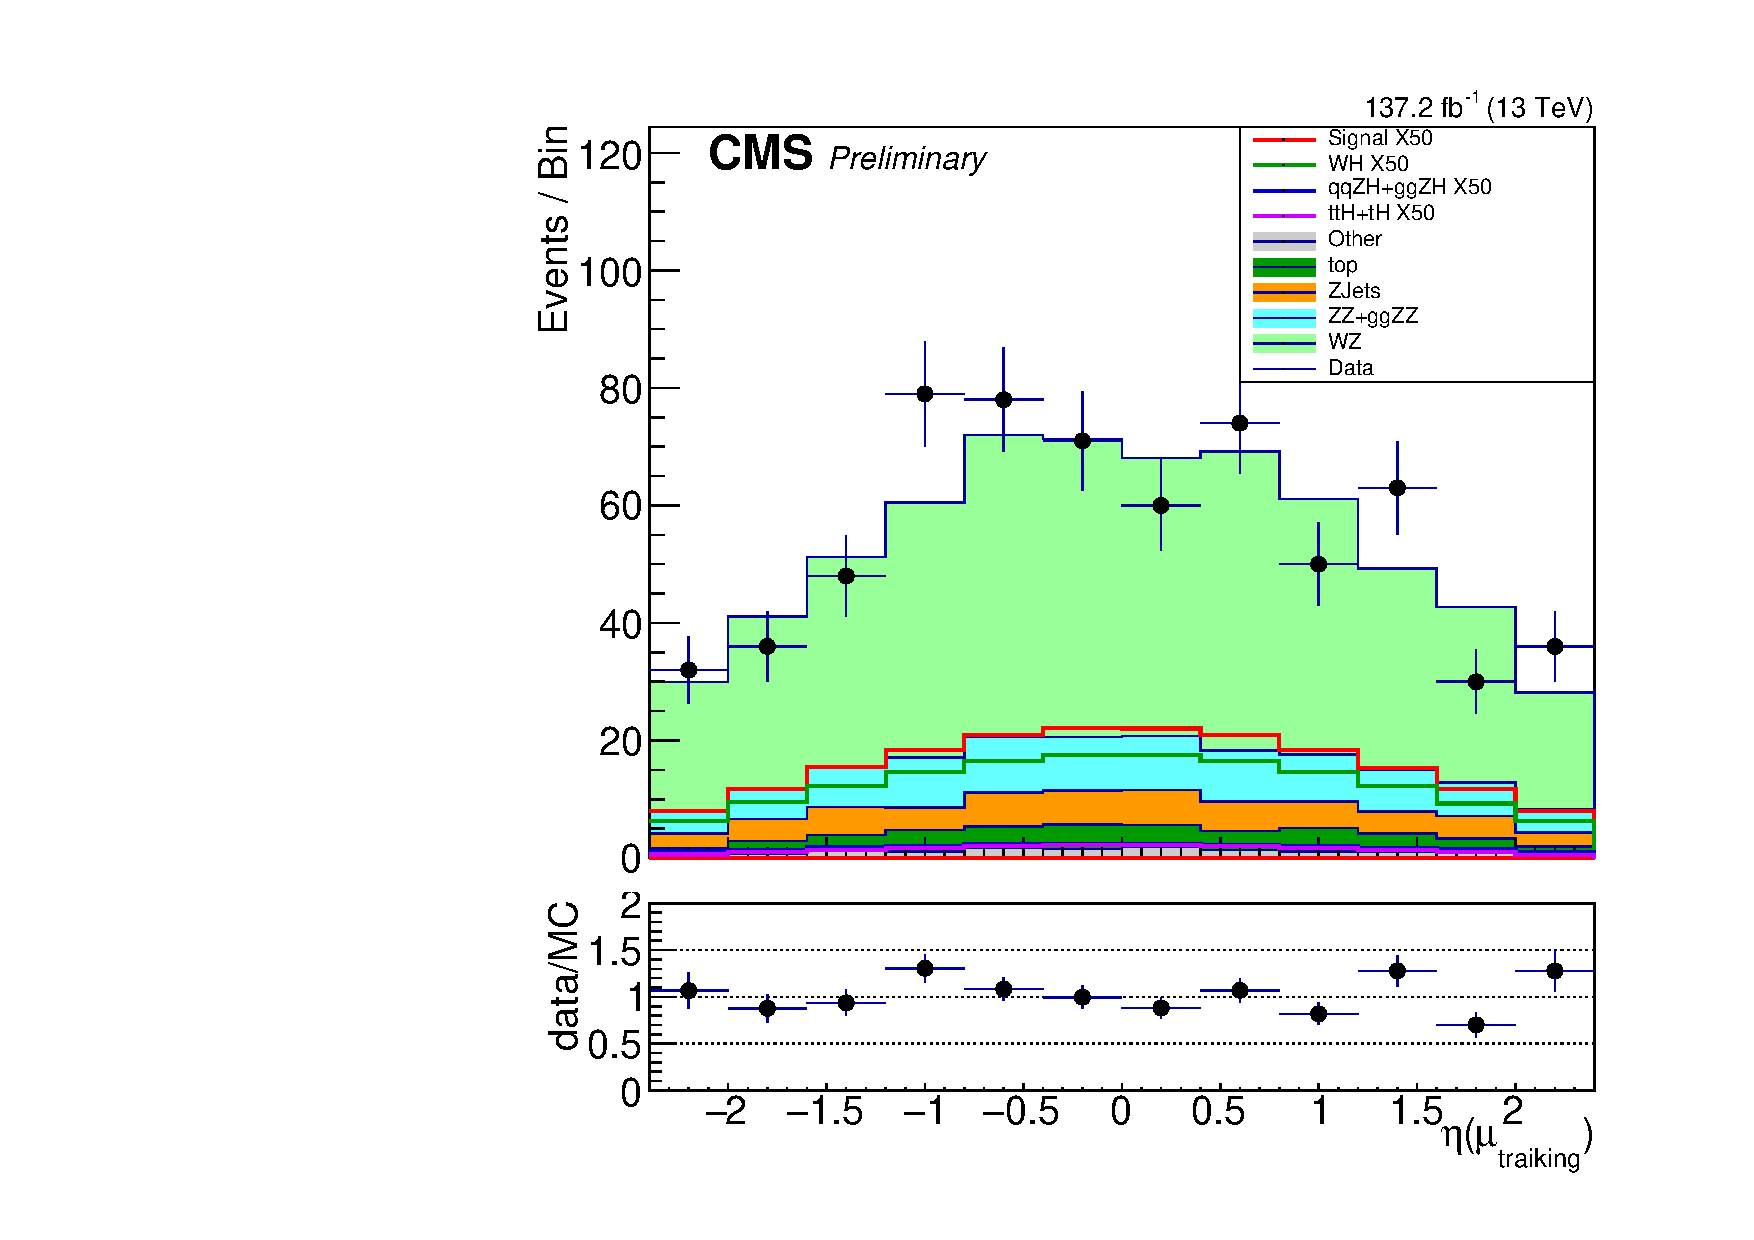
\includegraphics[width=0.24\textwidth]{pics/VH_sec/valid_BDT_WH/muH2_eta.pdf}
  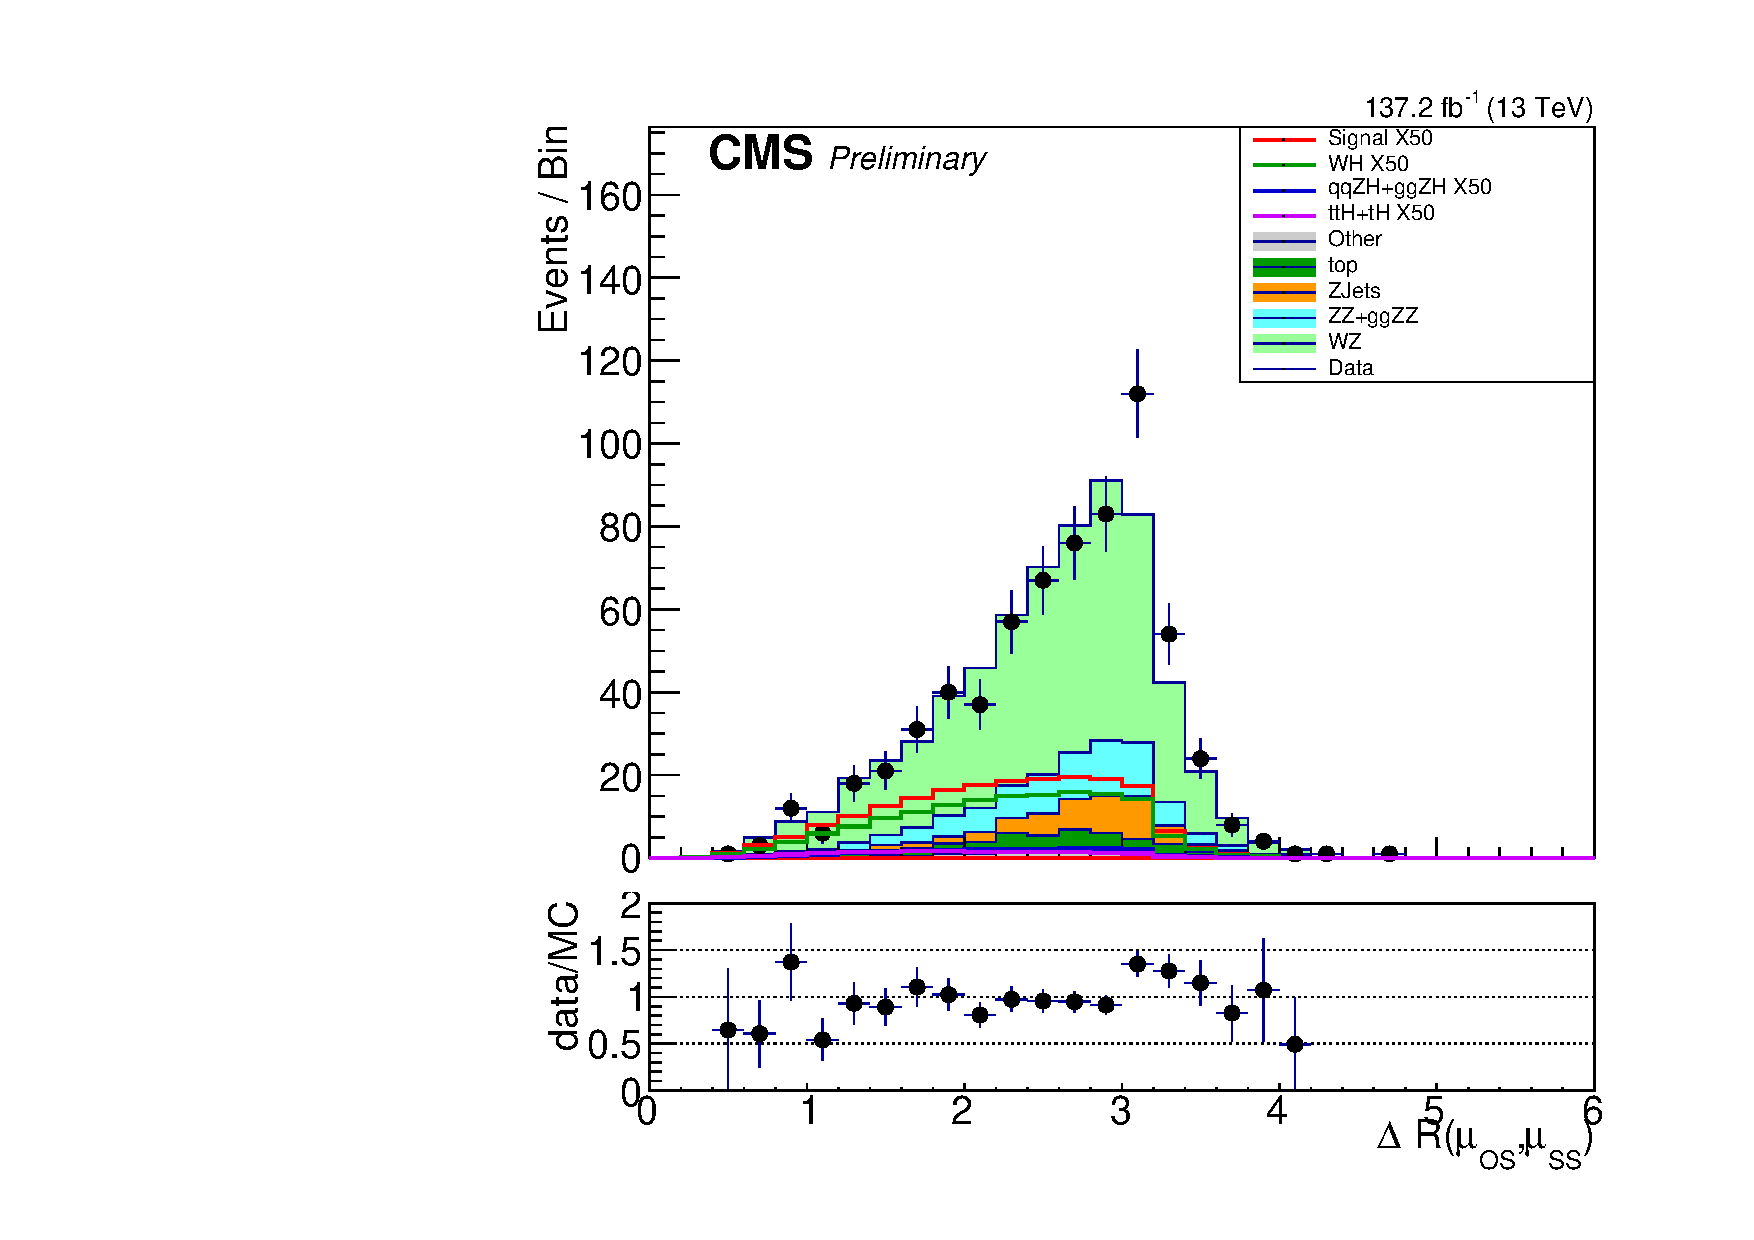
\includegraphics[width=0.24\textwidth]{pics/VH_sec/valid_BDT_WH/muSS_muOS_dR.pdf}
  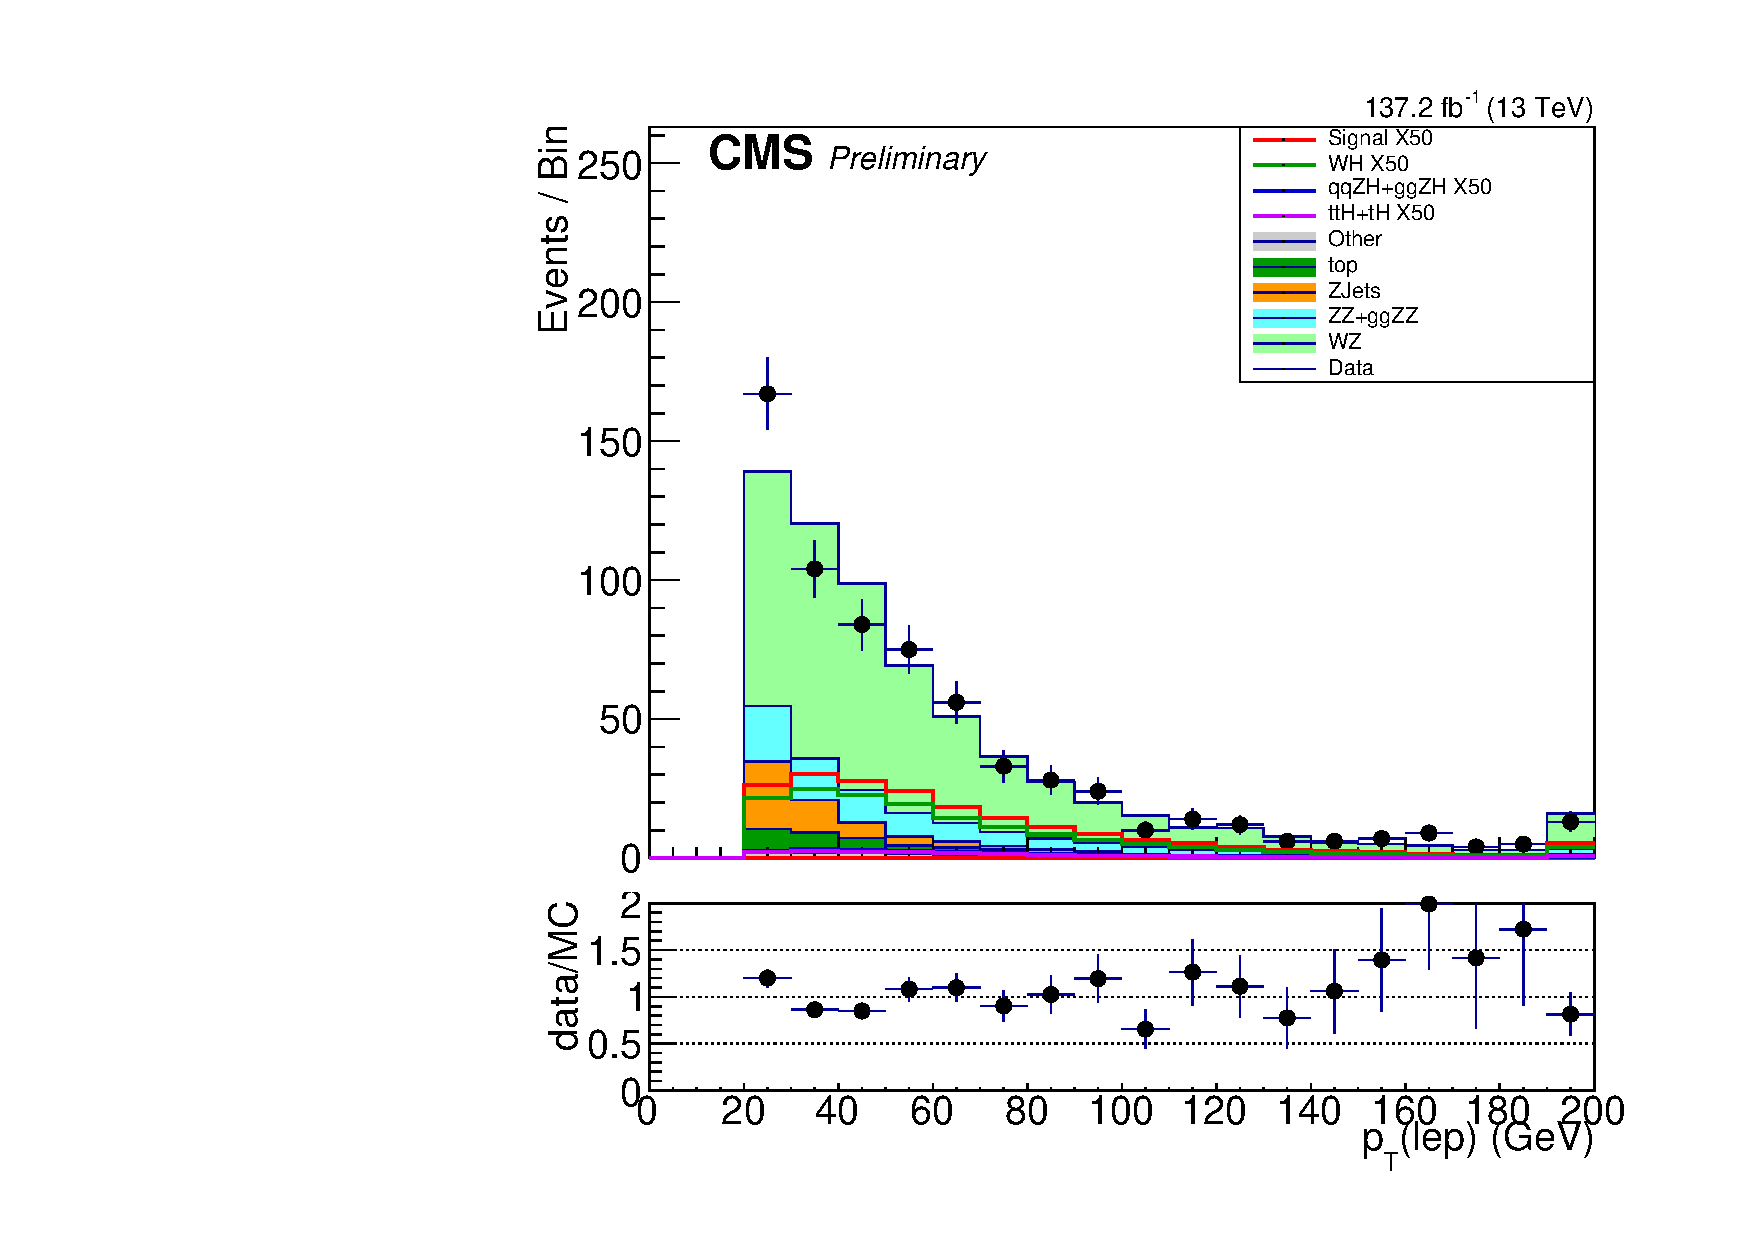
\includegraphics[width=0.24\textwidth]{pics/VH_sec/valid_BDT_WH/lep_pt.pdf}
  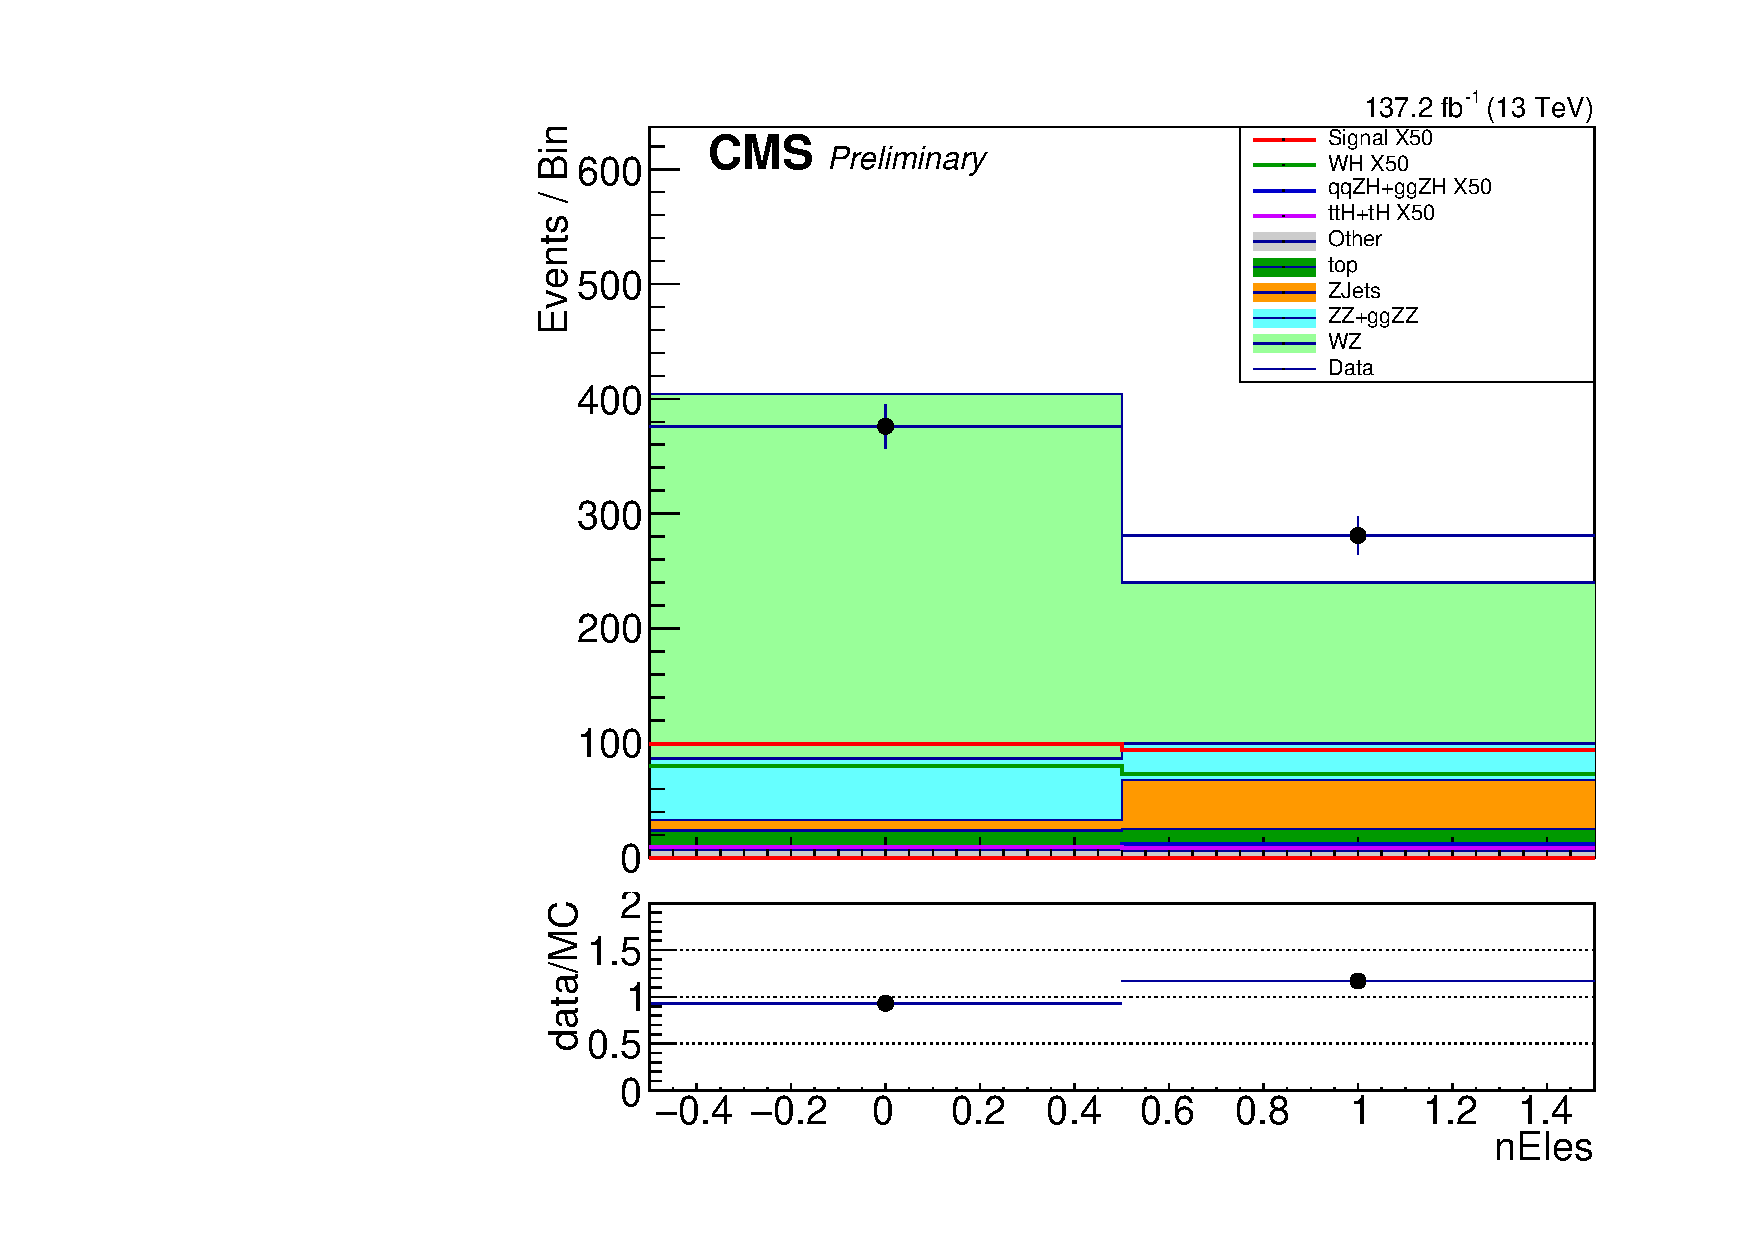
\includegraphics[width=0.24\textwidth]{pics/VH_sec/valid_BDT_WH/nEles.pdf}
  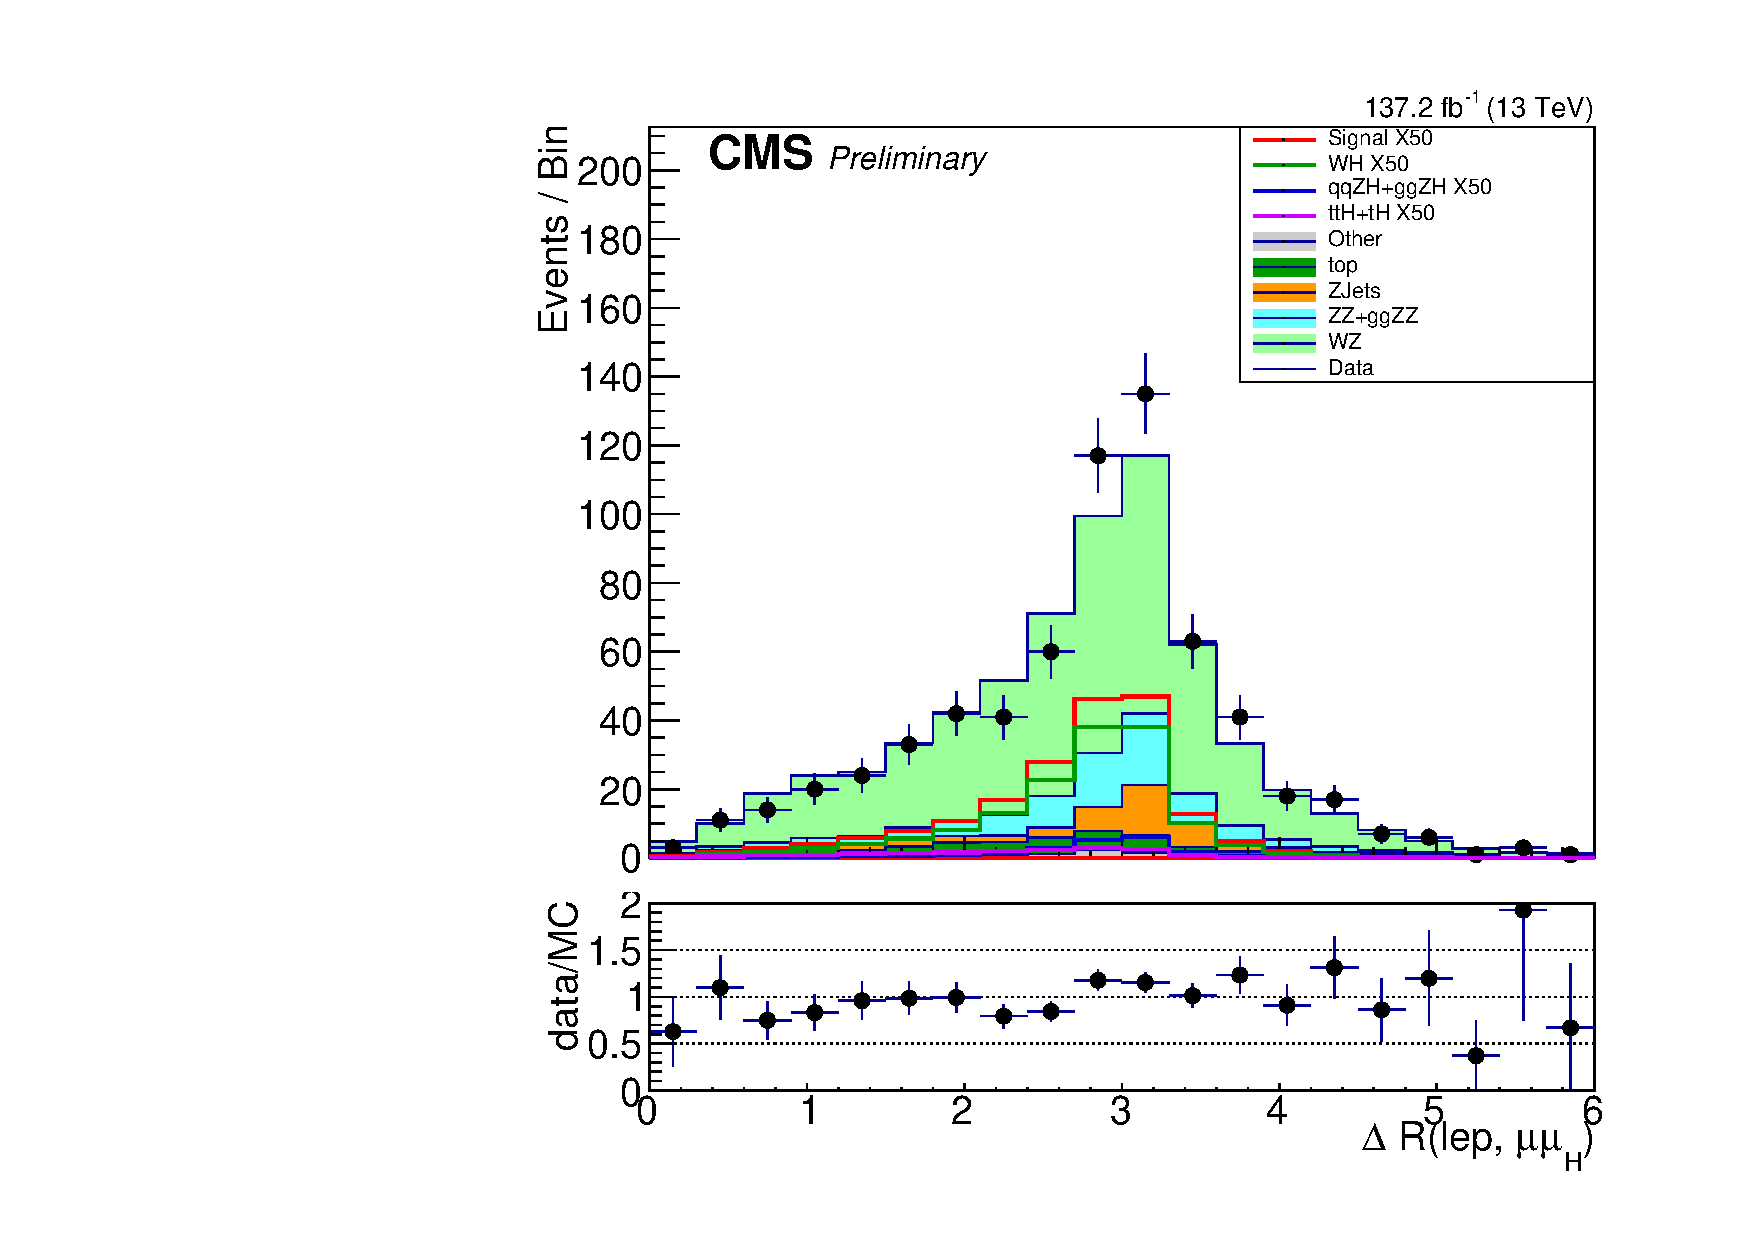
\includegraphics[width=0.24\textwidth]{pics/VH_sec/valid_BDT_WH/lep_H_pair_dR.pdf}
  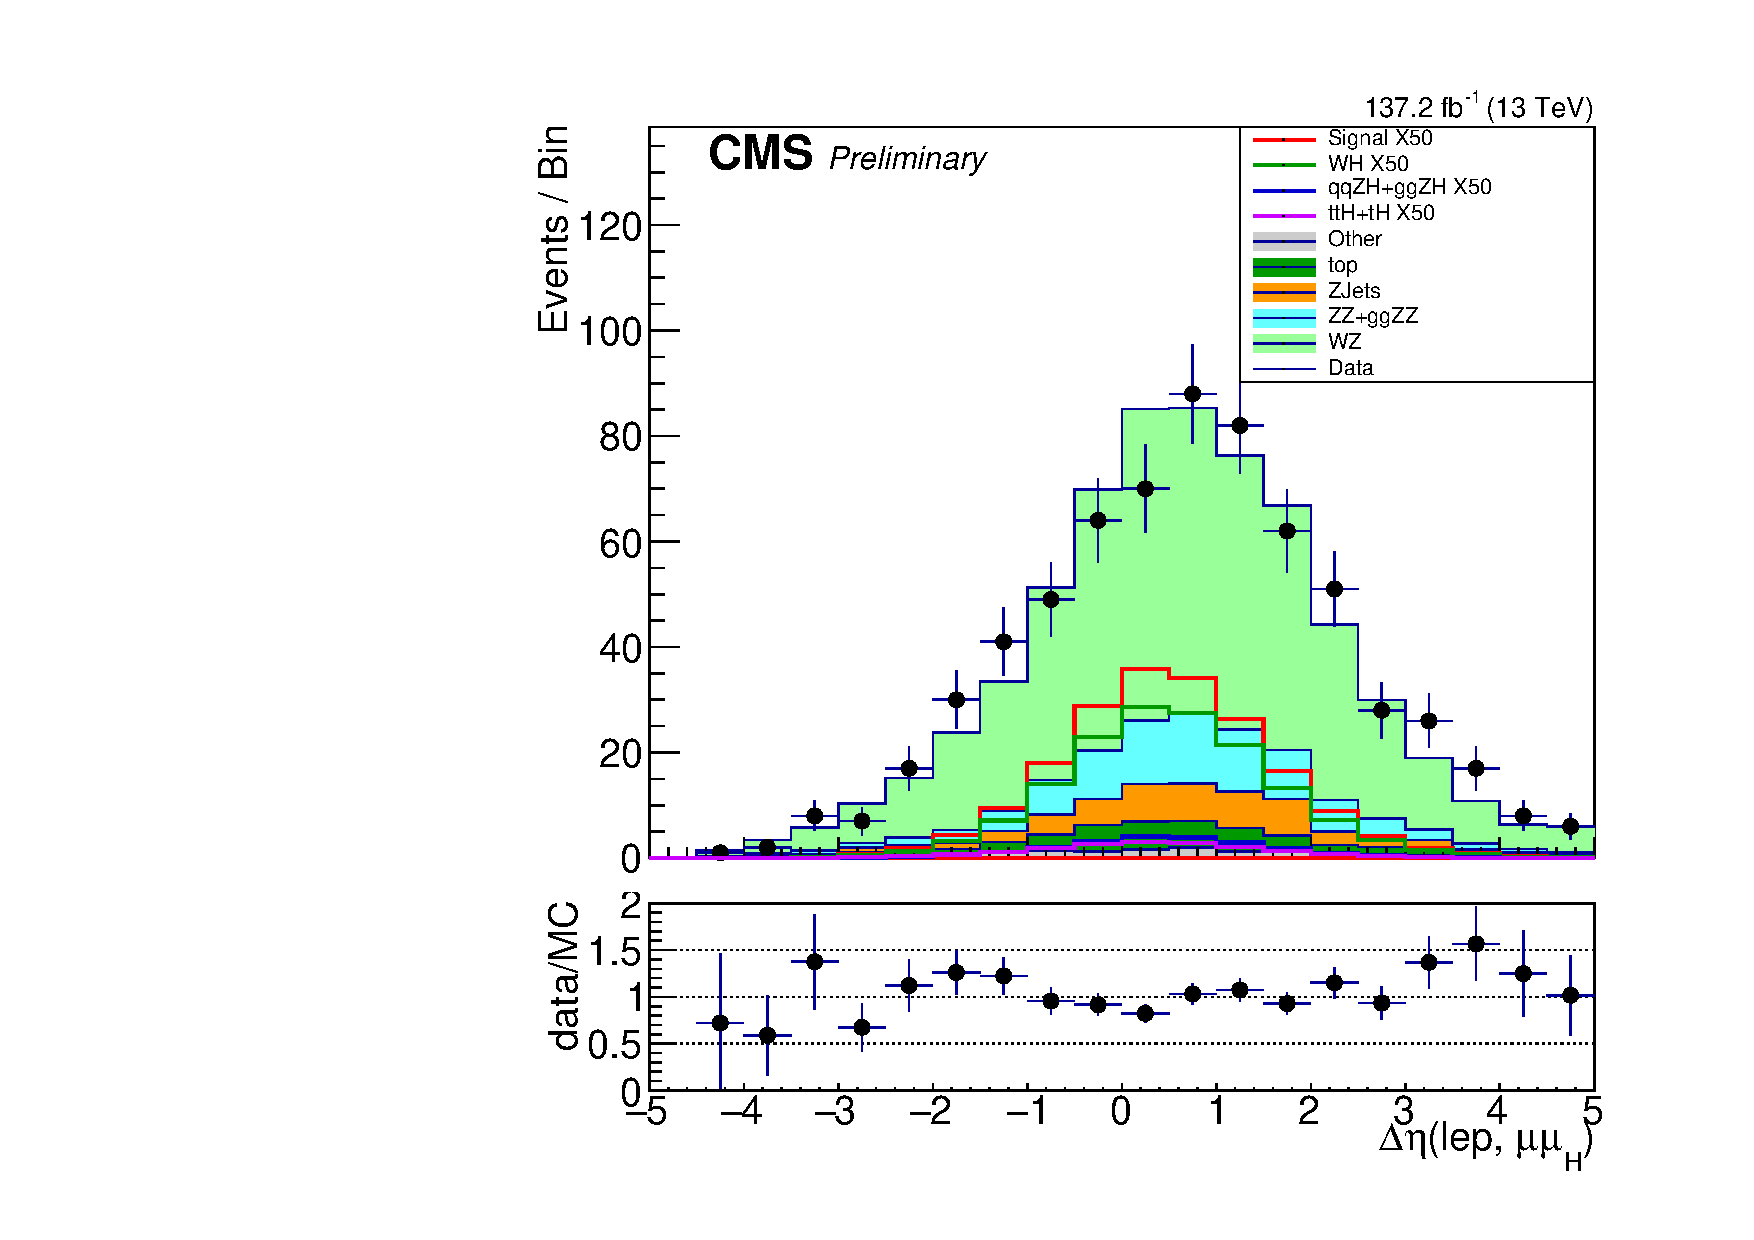
\includegraphics[width=0.24\textwidth]{pics/VH_sec/valid_BDT_WH/lep_H_pair_dEta.pdf}
  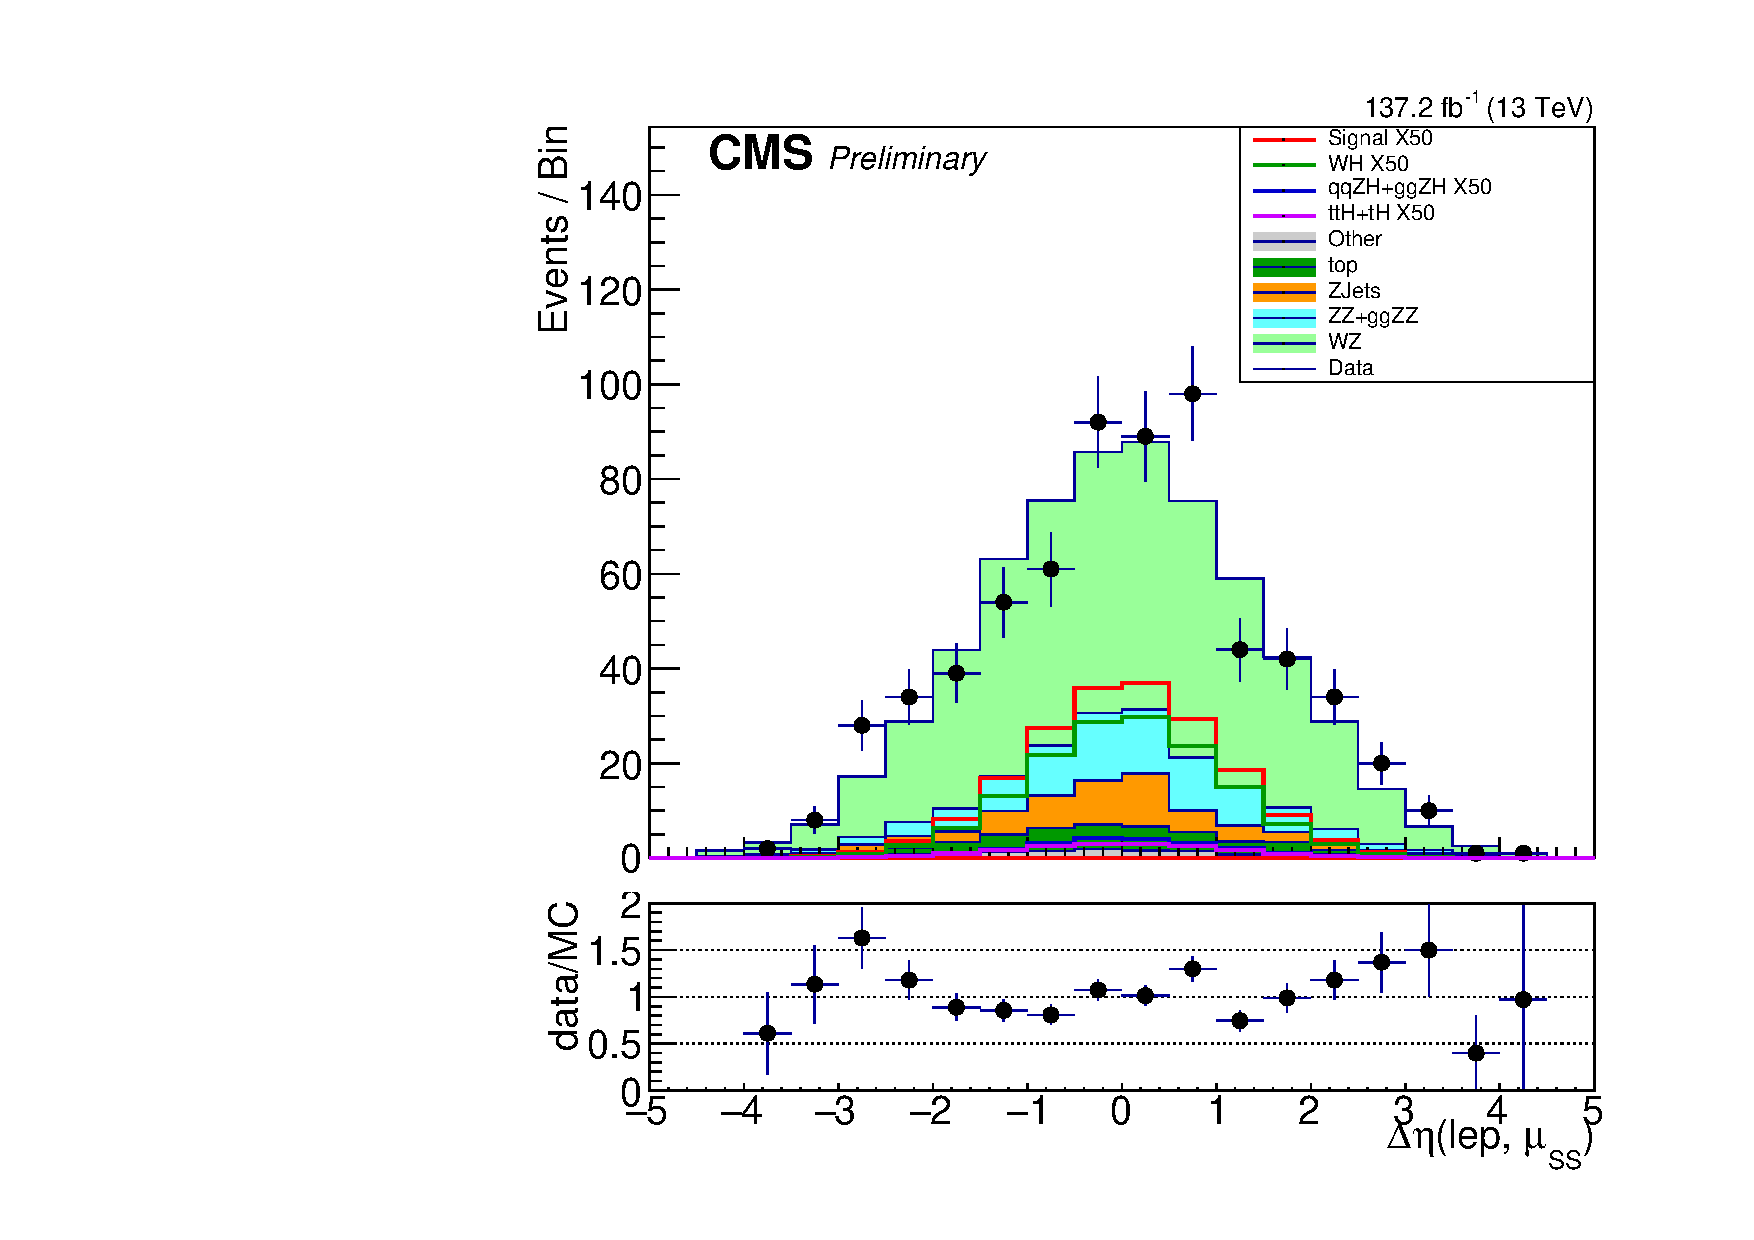
\includegraphics[width=0.24\textwidth]{pics/VH_sec/valid_BDT_WH/lep_muSS_dEta.pdf}
  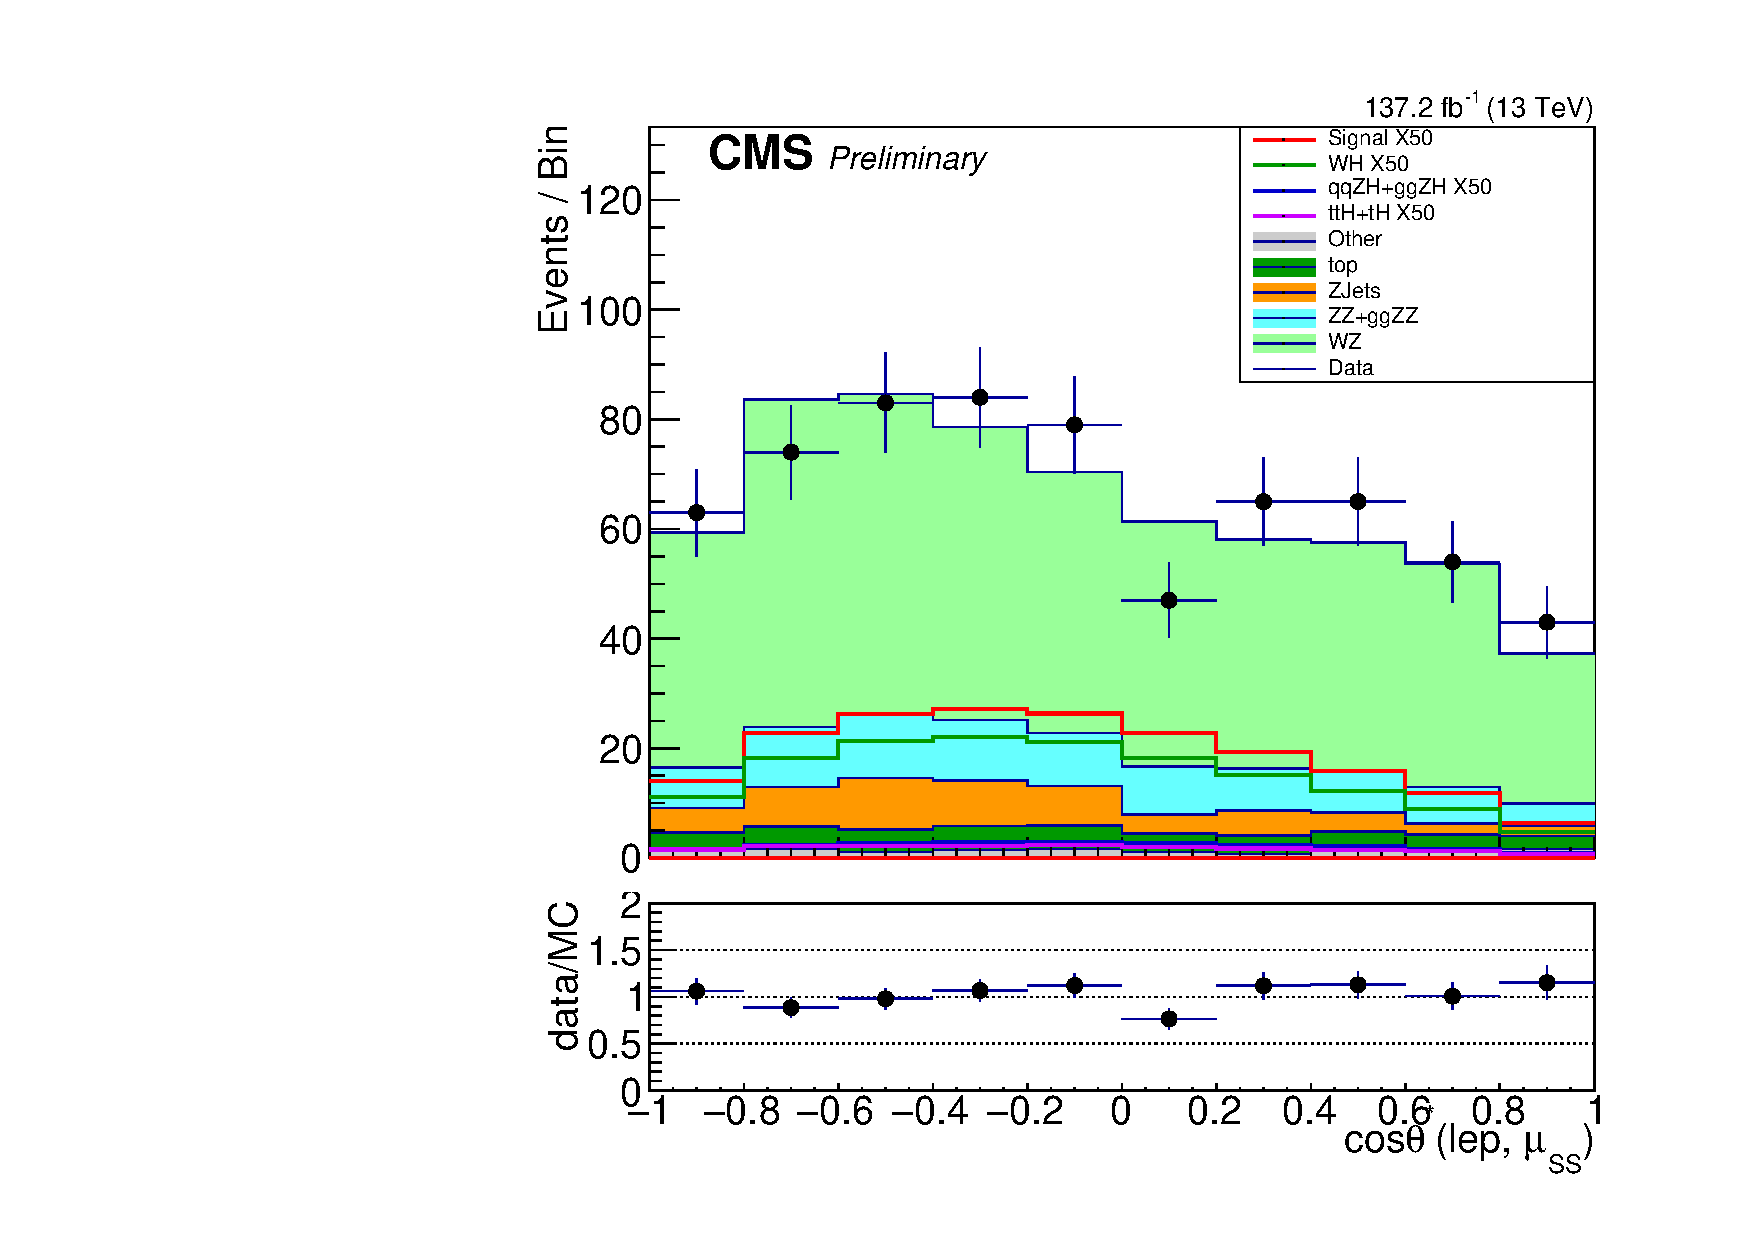
\includegraphics[width=0.24\textwidth]{pics/VH_sec/valid_BDT_WH/lep_muSS_cosThStar.pdf}
  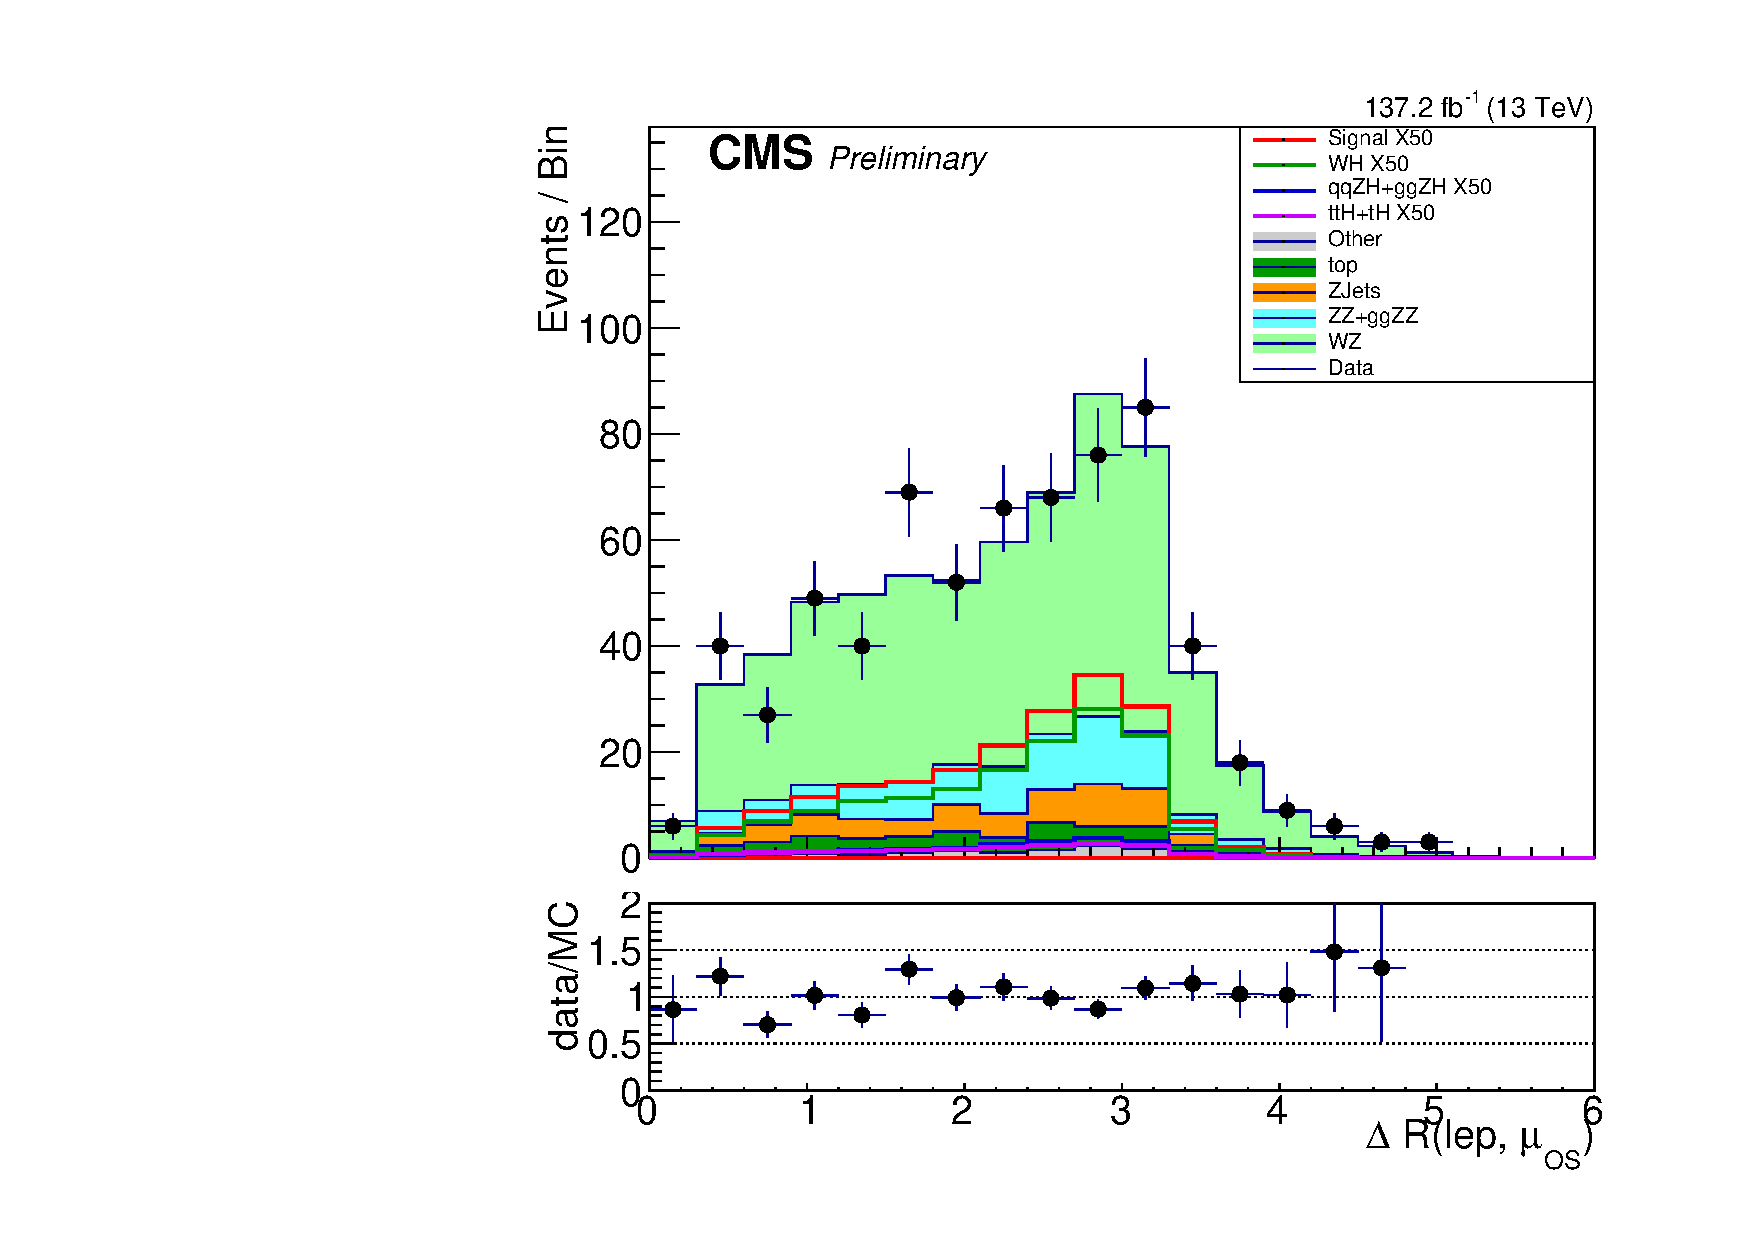
\includegraphics[width=0.24\textwidth]{pics/VH_sec/valid_BDT_WH/lep_muOS_dR.pdf}
  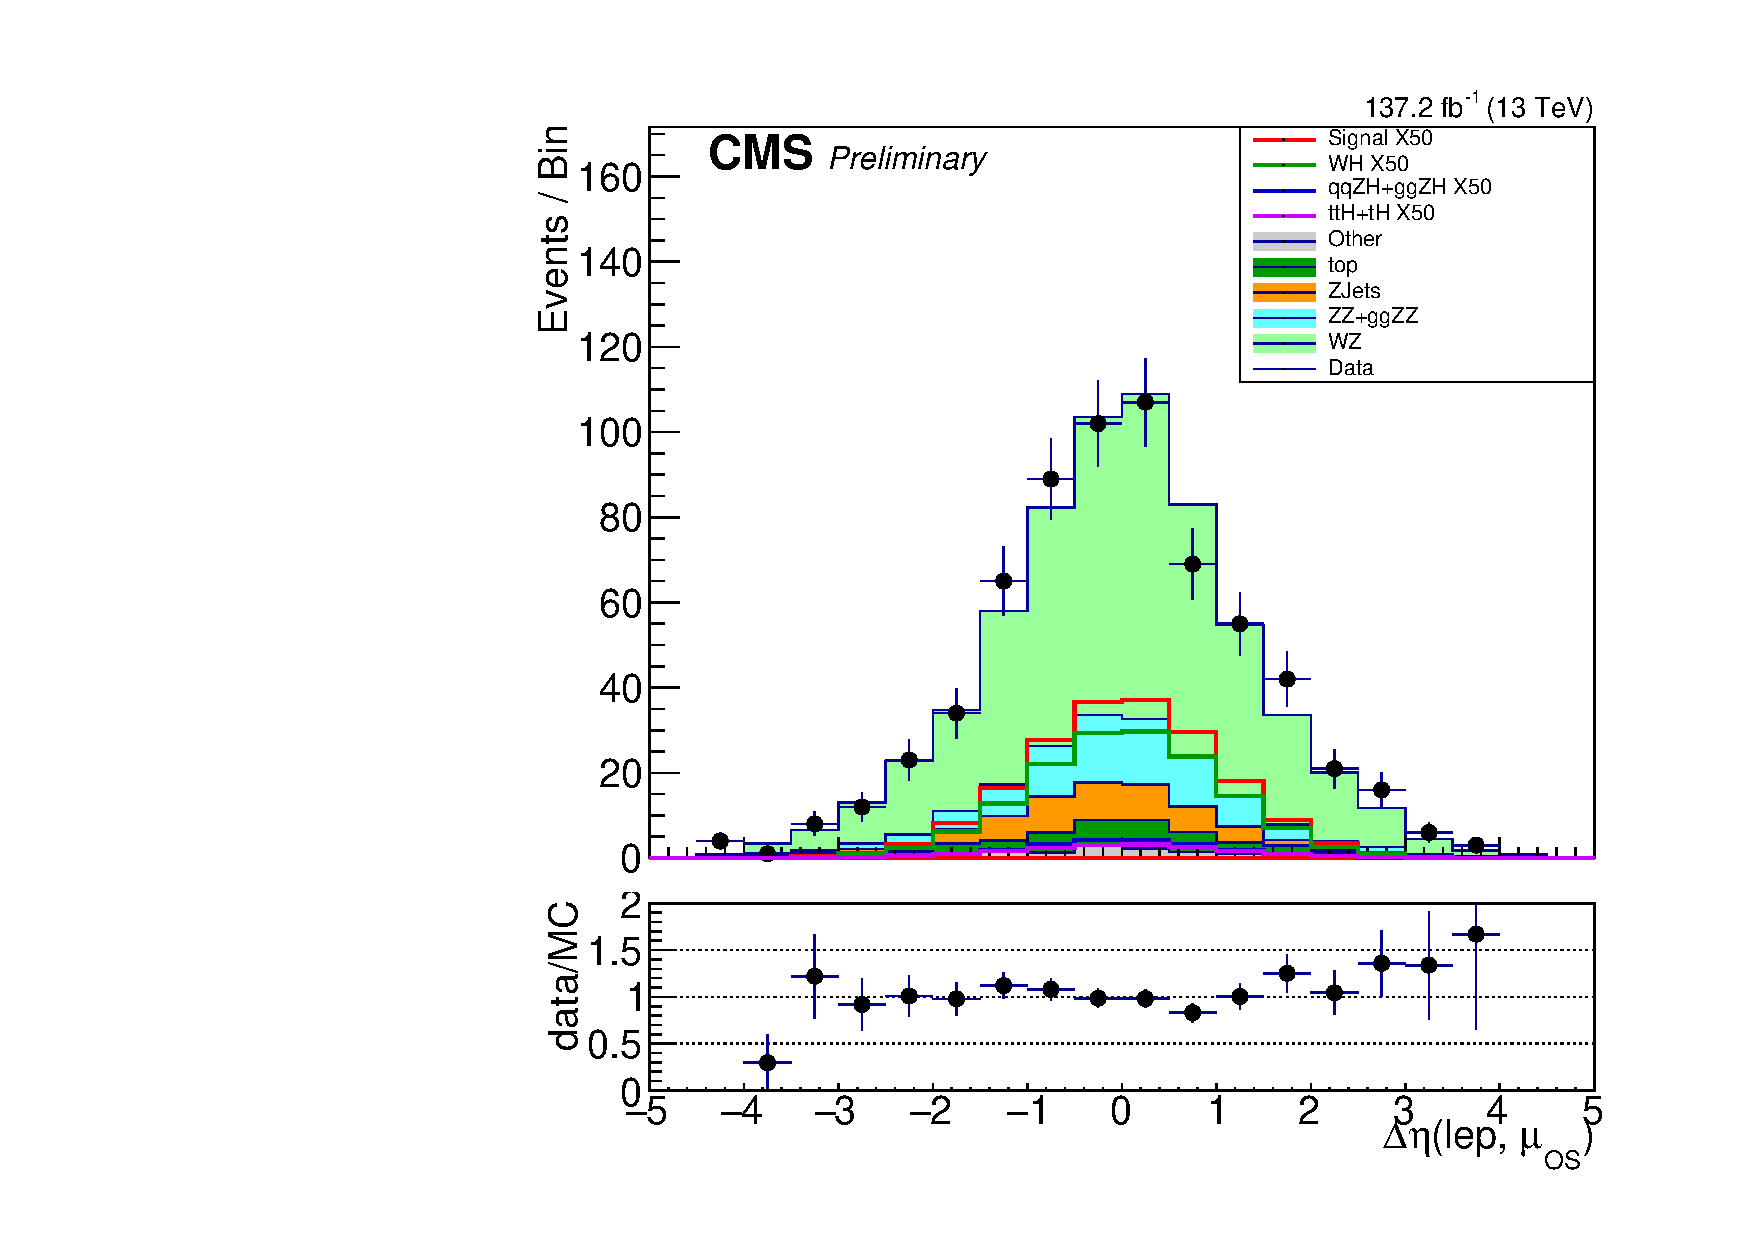
\includegraphics[width=0.24\textwidth]{pics/VH_sec/valid_BDT_WH/lep_muOS_dEta.pdf}
  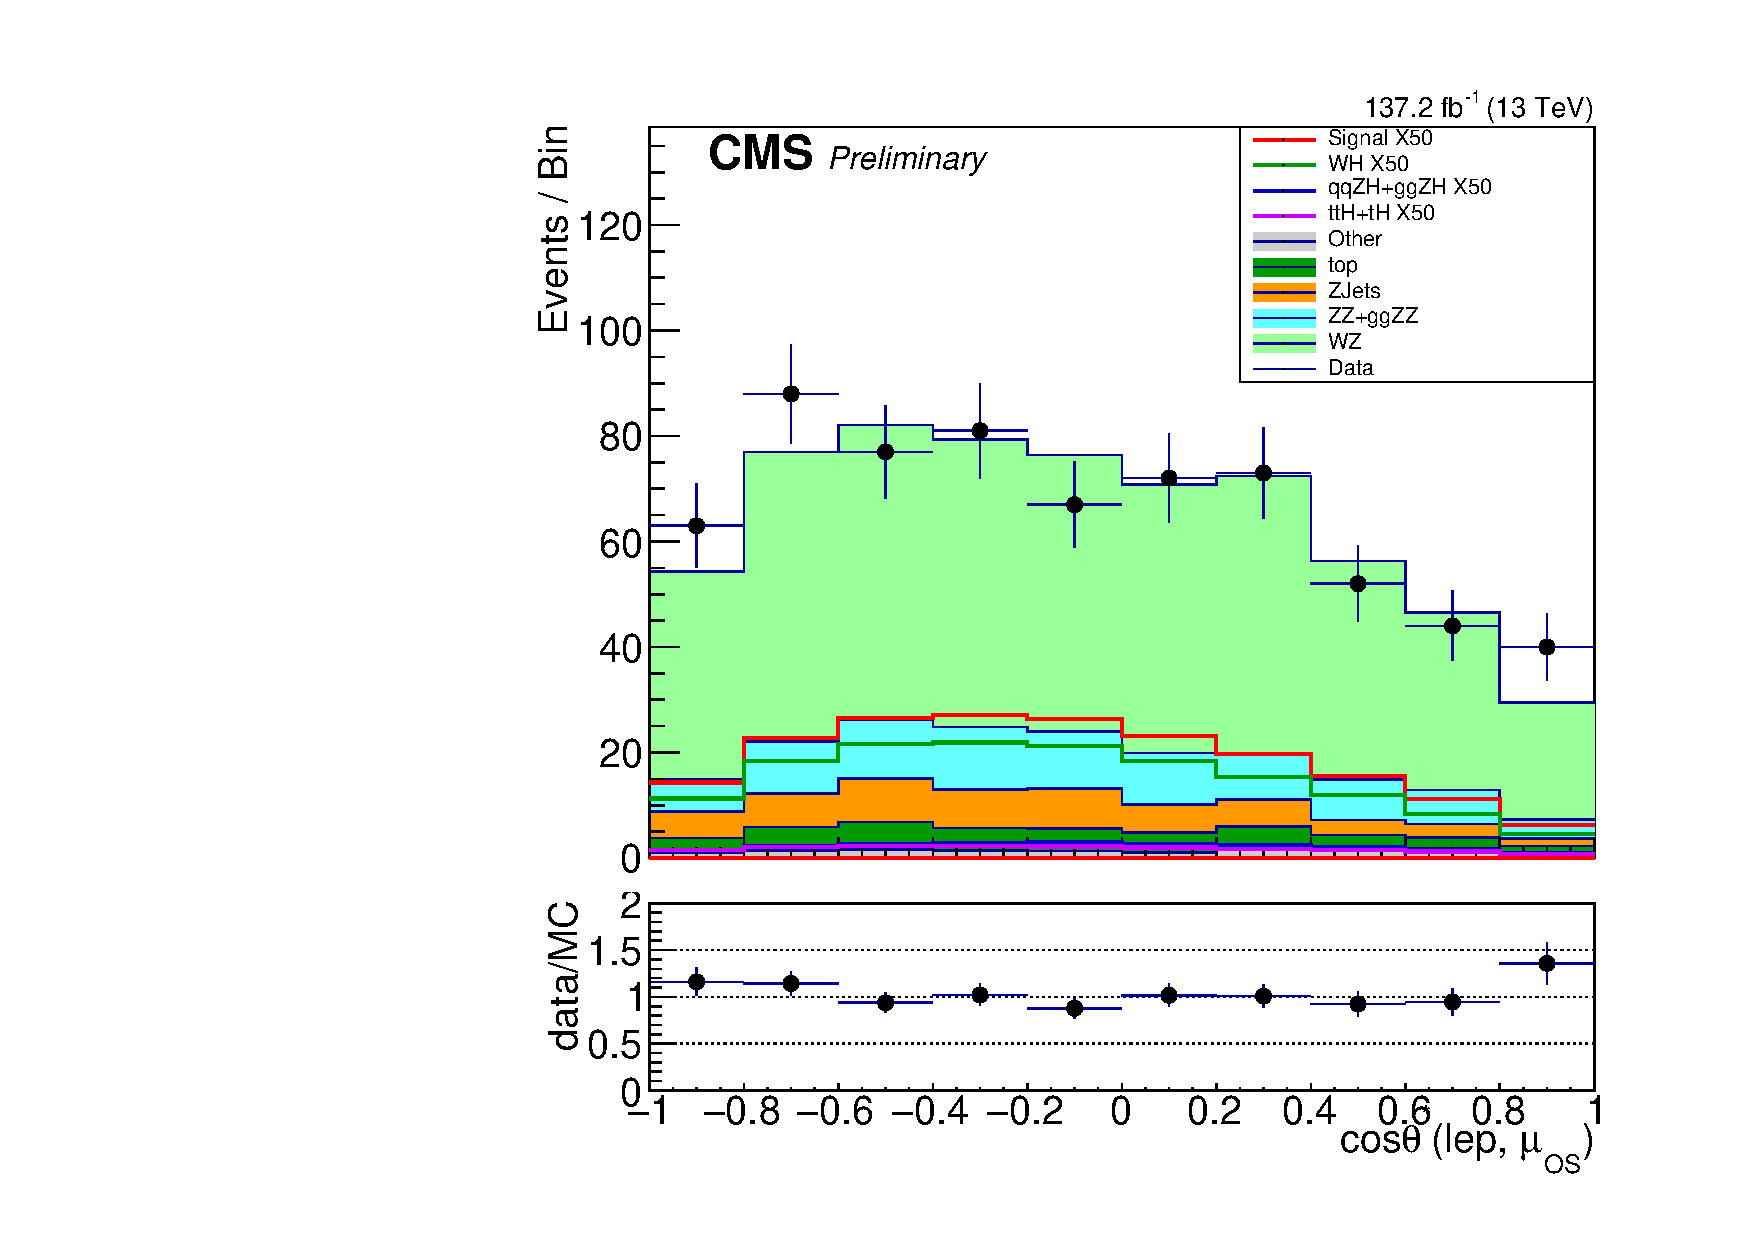
\includegraphics[width=0.24\textwidth]{pics/VH_sec/valid_BDT_WH/lep_muOS_cosThStar.pdf}
  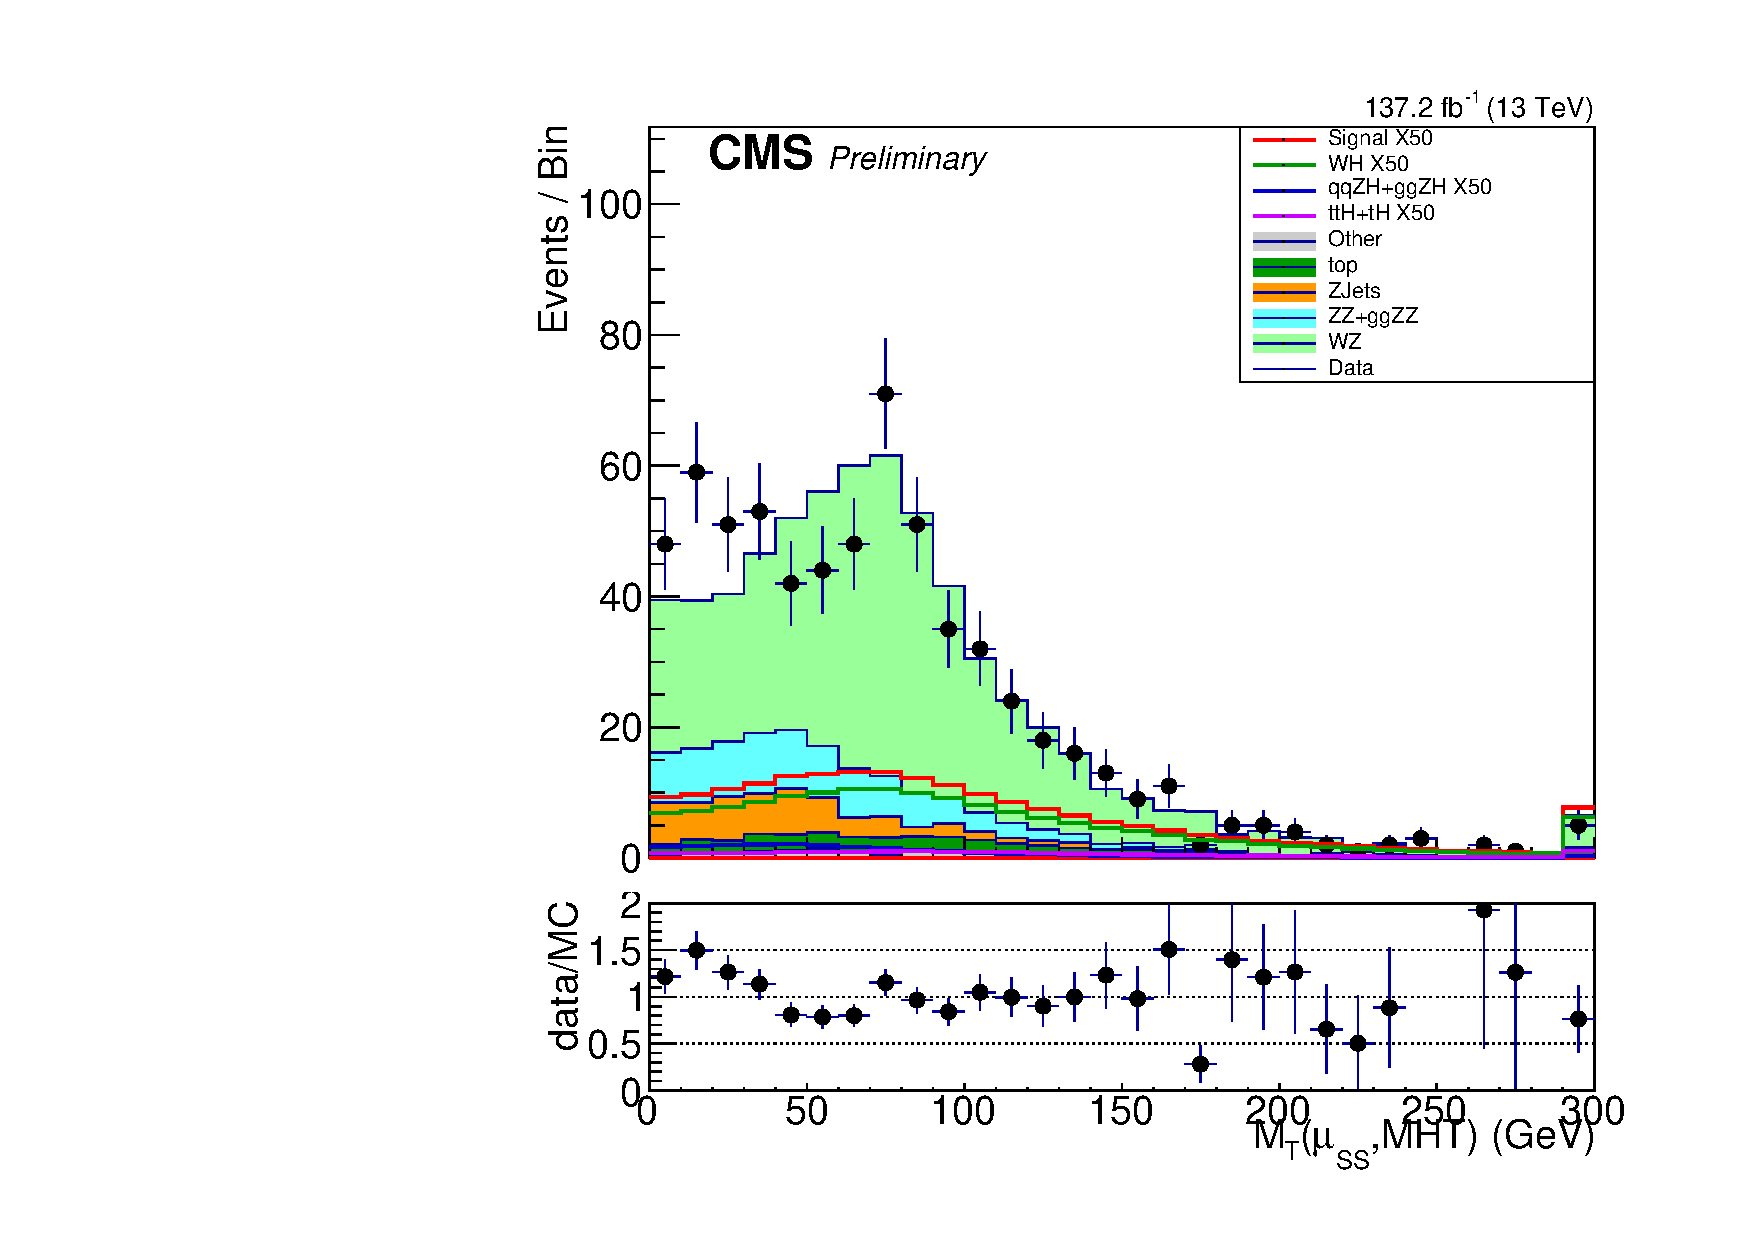
\includegraphics[width=0.24\textwidth]{pics/VH_sec/valid_BDT_WH/muSS_MHT_MT.pdf}
  \includegraphics[width=0.24\textwidth]{pics/VH_sec/valid_BDT_WH/lep_MHT_MT.pdf}
  \includegraphics[width=0.24\textwidth]{pics/VH_sec/valid_BDT_WH/lep_MHT_dPhi_abs.pdf}
  \caption{Input variables to the WH BDT in full Run 2 in the signal region 110 \GeV $<$ \mmm $<$ 150 \GeV.}
  \label{fig:wh_bdt_inputs_data}
\end{figure*}

\begin{figure*}[!htb]
  \centering
  \captionsetup{justification=justified}
  \includegraphics[width=0.24\textwidth]{pics/VH_sec/valid_BDT_ZH/dimu_pt.pdf}
  \includegraphics[width=0.24\textwidth]{pics/VH_sec/valid_BDT_ZH/dimu_abs_eta.pdf}
  \includegraphics[width=0.24\textwidth]{pics/VH_sec/valid_BDT_ZH/dimu_abs_dPhi.pdf}
  \includegraphics[width=0.24\textwidth]{pics/VH_sec/valid_BDT_ZH/dilep_mass.pdf}
  \includegraphics[width=0.24\textwidth]{pics/VH_sec/valid_BDT_ZH/dilep_pt.pdf}
  \includegraphics[width=0.24\textwidth]{pics/VH_sec/valid_BDT_ZH/dilep_abs_eta.pdf}
  \includegraphics[width=0.24\textwidth]{pics/VH_sec/valid_BDT_ZH/dilep_dR.pdf}
  \includegraphics[width=0.24\textwidth]{pics/VH_sec/valid_BDT_ZH/lep_ID.pdf}
  \includegraphics[width=0.24\textwidth]{pics/VH_sec/valid_BDT_ZH/cts_dipair_H.pdf}
  \includegraphics[width=0.24\textwidth]{pics/VH_sec/valid_BDT_ZH/dipair_dEta_H.pdf}
  \caption{Input variables to the ZH BDT in full Run 2 in the signal region 110 \GeV $<$ \mmm $<$ 150 \GeV.}
  \label{fig:zh_bdt_inputs_data}
\end{figure*}

An arguable disagreement is seen in the leftmost region in one of the inputs to the \WH BDT, $\MT(\mu_{SS}, $MHT$)$,
shown as the second plot in the bottom row of Figure~\ref{fig:wh_bdt_inputs_data}, also put separately in Figure~\ref{fig:wh_MT_check}. 
To understand if this disagreement would translate into a mismodeling of the \WH BDT, 
the BDT output is plotted for both signal and background in different $\MT(\mu_{SS}, $MHT$)$ bins, 
shown as the right plot in Figure~\ref{fig:wh_MT_check}.
In this plot, for both signal and background, 
the BDT profile is almost the same for events with $\MT(\mu_{SS}, $MHT$)$ $<$ 40 \GeV and events with 40 $<$ $\MT(\mu_{SS}, $MHT$)$ $<$ 80 \GeV,
while it is different between events with $\MT(\mu_{SS}, $MHT$)$ $<$ 80 \GeV from events with $\MT(\mu_{SS}, $MHT$)$ $>$ 80 \GeV.  
The BDT is sensitive to whether the $\MT(\mu_{SS}, $MHT$)$ is greater or smaller than 80 \GeV, 
but does not further distinguish events if the $\MT(\mu_{SS}, $MHT$)$ is less than 80 \GeV.
Once the bins below 80 \GeV are merged in the left plot of Figure~\ref{fig:wh_MT_check}, there is no significant disagreement, 
therefore it should not cause any mismodeling of the BDT.

\begin{figure*}[!htb]
  \centering
  \captionsetup{justification=justified}
  \includegraphics[width=0.42\textwidth]{pics/VH_sec/valid_BDT_WH/muSS_MHT_MT.pdf}
  \includegraphics[width=0.42\textwidth]{pics/VH_sec/valid_BDT_WH/check_MT_plot.png}
  \caption{The input variable $\MT(\mu_{SS}, $MHT$)$ to the \WH BDT (left), 
           and the BDT output for signal and background in different $\MT(\mu_{SS}, $MHT$)$ bins (right).
           A mild disagreement is seen between the simulation and data in the low bins of $\MT(\mu_{SS}, $MHT$)$,
           while the BDT is not sensitive to the $\MT(\mu_{SS}, $MHT$)$ values in that region.}
  \label{fig:wh_MT_check}
\end{figure*}

\clearpage
\section{Event Categorization}\label{sec:vh_event_cats}

To optimize the overall sensitivity of the VH analyses, 
the \WH and the \ZH phase-spaces are divided into several subcategories with different S/B ratios, 
based on the BDT discriminants described in Section~\ref{sec:vh_bdt_cats}. 
 
To achieve the maximal sensitivity with a reasonable number of subcategories, 
an iterative procedure is taken.  
In each iteration, a cut is scanned at a step of 0.01 of the BDT value and the sum of
the significance of the resulting subcategories is calculated as the figure of merit. 
The figure of merit is defined as the $\mathrm{S}/\sqrt{\mathrm{B}}$ in each subcategory 
summed in quadrature, where $\mathrm{S}$ and $\mathrm{B}$ represent the expected 
signal and background yields within the full width at half maximum (FWHM) of the signal peak in each subcategory.
In addition, to ensure that there are enough events in each subcategory to perform a shape analysis,
all subcategories have to meet a minimal total event yield requirement during the BDT scanning process.
The choice of this minimal requirement is somewhat arbitrary,
and is determined based on the experience with the subsequent "bias studies" described in Section~\ref{sec:bias_study}.
This number is chosen to be 30 in the \WH BDT scans,
and 16 in the \ZH BDT scans, as the total number of events in the \ZH category is less than 50. 

\begin{figure*}[!htb]
  \centering
  \captionsetup{justification=justified}
  \includegraphics[width=0.32\textwidth]{pics/VH_sec/VH_BDT_cats/WH_BDT_scan1.pdf}
  \includegraphics[width=0.32\textwidth]{pics/VH_sec/VH_BDT_cats/WH_BDT_scan2.pdf}
  \includegraphics[width=0.32\textwidth]{pics/VH_sec/VH_BDT_cats/WH_BDT_scan3.pdf}
  \caption{Scans for the first (left), second (middle) and a potential third (right) BDT cut in the WH channel.
           The first BDT cut is chosen at 0.3. The second BDT cut is chosen at -0.1. A third BDT cut is not necessary.}
  \label{fig:wh_bdt_cat_scan}
\end{figure*}

Figure~\ref{fig:wh_bdt_cat_scan} shows the iterations performed on the \WH BDT. 
In the first scan, the overall significance maximizes around $0 \sim 0.3$, 
and the cut is chosen at 0.3 so that there are enough events on its left side for a second cut.
In the second scan, the overall significance maximizes around $-0.1 \sim 0.05$,
and the position of the second cut can be any value in this range.
To help decide the second cut, several third scans are performed under different assumptions of the second cut,
all showing negligible changes of the overall significance (similar to the right plot in Figure~\ref{fig:wh_bdt_cat_scan}).
Therefore, there is no need for a third cut, and the choice for the second cut can be somewhat arbitrary.
The second cut is decided at -0.1 so that there are a good number of events in the middle subcategory to ensure a stable shape analysis.  
As a result, two BDT boundaries are set, dividing the WH phase-space into 3 subcategories, 
BDT within [-1.0, -0.1], BDT within [-0.1, 0.3] and BDT within [0.3, 1.0].

\begin{figure*}[!htb]
  \centering
  \captionsetup{justification=centering}
  \includegraphics[width=0.32\textwidth]{pics/VH_sec/VH_BDT_cats/ZH_BDT_scan.pdf}
  \caption{Scans for the BDT cut in the \ZH channel. The BDT cut is chosen at -0.1.}
  \label{fig:zh_bdt_cat_scan}
\end{figure*}

Similarly, Figure~\ref{fig:zh_bdt_cat_scan} shows the scan performed on the \ZH BDT. 
In the BDT scan, the overall significance maximizes around $-0.15 \sim 0.05$.
The BDT cut is chosen at -0.1, dividing the \ZH events into two roughly equal halves.
A second cut is not needed as the number of events is not enough for a further division.
The resulting 2 \ZH subcategories are, BDT within [-1.0, -0.1], and BDT within [-0.1, 1.0].


\section{Signal and background modeling}\label{sec:vh_sig_bkg_model}

The extraction of signal is performed by fitting analytic functions to the \mmm spectrum in each subcategory.
Different functions are used to model the expected signal and background shapes: a sharp signal peak near 125 \GeV,
and a smooth falling background shape in $110 ~\GeV{} < \mmm < 150 ~\GeV{}$.
Functions are first tested on the simulated samples to make sure the perform well in describing the shapes.
The parameters of the signal function are constrained, with systematic uncertainties described in Section~\ref{sec:shape_uncertainty},
to the best fit values to simulation as the expectation of the SM signal.
The parameters of the background function are allowed to float freely, so that no prior assumption on the background is imposed,
and the background prediction relies completely on data.
The final evaluation of the signal strength is achieved by fitting the signal + background functions to data.
where the normalizations of both the signal function and the background function are allowed to float freely.
The normalization of the signal, in particular, is called the signal strength modifier and represents the signal strength relative to the SM prediction.

Function modeling of signal and background are described in Sections~\ref{sec:vh_sig_model} and ~\ref{sec:vh_bkg_model} respectively.

\subsection{Signal modeling}\label{sec:vh_sig_model}
In all subcategories, signals are modeled independently by different production modes,
with the contributions from three years (2016, 2017, 2018) summed together. 
In particular, \qqZH and \ggZH signals are modeled separately as there are no other signal component in the \ZH category.
Each of the components is modeled with a Double-sided Crystal Ball function (DCB), as described in Equation~\ref{eq:dCBFunction}.  
In all DCB functions, the parameters $n_L$ and $n_R$ are fixed to 2.0, 
since they only affect the shape in tails and can take values in a large range without changing the quality of the fit by much. 
Other parameters are allowed to float freely.  

\begin{equation}
  \label{eq:dCBFunction}
  \text{DCB}(m_{\mu\mu})=%
    \begin{cases}
        e^{-(m_{\mu\mu} - s)^{2}/(2\sigma^{2})} & \ \ -\alpha_{\mathrm{L}} < (m_{\mu\mu}-s)/\sigma < \alpha_{\mathrm{R}} \\
        (\frac{n_{\mathrm{L}}}{|\alpha_{\mathrm{L}}|})^{n_{\mathrm{L}}} \times e^{-\alpha^{2}_{\mathrm{L}}/2} \times (\frac{n_{\mathrm{L}}}{|\alpha_{\mathrm{L}}|} - |\alpha_{\mathrm{L}}| - (m_{\mu\mu}-s)/\sigma)^{-n_{\mathrm{L}}}
        & \ \ (m_{\mu\mu}-s)/\sigma \leq -\alpha_{\mathrm{L}} \\
        (\frac{n_{\mathrm{R}}}{|\alpha_{\mathrm{R}}|})^{n_{\mathrm{R}}} \times e^{-\alpha^{2}_{\mathrm{R}}/2} \times (\frac{n_{\mathrm{R}}}{|\alpha_{\mathrm{R}}|} - |\alpha_{\mathrm{R}}| + (m_{\mu\mu}-s)/\sigma)^{-n_{\mathrm{R}}}
        & \ \ (m_{\mu\mu}-s)/\sigma \geq \alpha_{\mathrm{R}} \\
    \end{cases}
\end{equation}

Examples of signal modeling are shown in Figures~\ref{fig:signal_models_in_WH3l} and ~\ref{fig:ZH_signal_model_in_ZH4l}. 
Please note that the plots shown are the signals in the inclusive \WH and \ZH categories. 
The actual models used in each subcategory are slightly different. 
\ggH, \qqH and \bbH have negligible contributions to the WH category and are not considered.  
Similarly, in the ZH category only \qqZH and \ggZH are considered since all other contributions are negligible. 

\begin{figure*}[!htb]
  \centering
  \captionsetup{justification=justified}
  \includegraphics[width=0.32\textwidth]{pics/VH_sec/WH_signal_models//WH_CatAll_fit_DSCB_1.png}
  \includegraphics[width=0.32\textwidth]{pics/VH_sec/WH_signal_models/qqZH_CatAll_fit_DSCB_1.png}
  \includegraphics[width=0.32\textwidth]{pics/VH_sec/WH_signal_models/ggZH_CatAll_fit_DSCB_1.png}
  \includegraphics[width=0.32\textwidth]{pics/VH_sec/WH_signal_models/ttH_CatAll_fit_DSCB_1.png}
  \includegraphics[width=0.32\textwidth]{pics/VH_sec/WH_signal_models/THQ_CatAll_fit_DSCB_1.png}
  \includegraphics[width=0.32\textwidth]{pics/VH_sec/WH_signal_models/THW_CatAll_fit_DSCB_1.png}
  \caption{The signal modeling in the WH $\to \ell+\mu\mu$ inclusive category. Considered signal modes are WH (top left), 
           qqZH (top middle), ggZH (top right), ttH (bottom left), THQ (bottom middle), and THW (bottom right).}
  \label{fig:signal_models_in_WH3l}
\end{figure*}

\begin{figure*}[!htb]
  \centering
  \captionsetup{justification=justified}
  \includegraphics[width=0.32\textwidth]{pics/VH_sec/ZH_signal_models/qqZH_CatAll_fit_DSCB_1.png}
  \includegraphics[width=0.32\textwidth]{pics/VH_sec/ZH_signal_models/ggZH_CatAll_fit_DSCB_1.png}
  \caption{The signal modeling in the ZH $\to \ell\ell+\mu\mu$ inclusive category. Considered signals modes are 
           qqZH (left) and ggZH (right).}
  \label{fig:ZH_signal_model_in_ZH4l}
\end{figure*}


\subsection{Background modeling}\label{sec:vh_bkg_model}

As discussed in Section~\ref{sec:vh_event_selection}, the main background in \WH (\ZH) category is the \WZ (\ZZ) process, 
a fraction of which consists wrong pairing of the muons.
The \mmm spectrum of the correctly paired \WZ (\ZZ) events follows a Breit-Wigner tail of the \PZ boson, 
while the spectrum of the wrongly paired \WZ (\ZZ) events is rather flat.
Overall the background shapes in the \WH and \ZH categories are smoothly falling, and Breit-Wigner like to some extent.
Therefore, a group of different functional forms are considered as candidates for the background modeling.
Some of them are physics-inspired, meaning that they are modified from the form of the Breit-Wigner function, 
the others are agnostic that take the form of some general functional bases.
The physics-inspired function candidates include the $BWZ$ function (Equation~\ref{eq:BWZ}), which is a Breit-Wigner core times an exponential term , 
the $BWZRedux$ (Equation~\ref{eq:BWZRedux}), which is a Breit-Wigner core times a exponential term with more degrees of freedom (DOFs),
the $BWZGamma$ (Equation~\ref{eq:BWZGamma}), which is a linear combination of the $BWZ$ function and an exponential function,
and the $BWZ \times Bernstein$ (Equation~\ref{eq:BWZBern}), which is the $BWZ$ function times a Bernstein polynomial. 


\begin{equation}\label{eq:BWZ}
   \mathrm{BWZ}(m_{\mu\mu}) = \frac{\Gamma_{\mathrm{Z}} \cdot e^{a\cdot m_{\mu\mu}}}{(m_{\mu\mu}-m_{\mathrm{Z}})^2+(\Gamma_{\mathrm{Z}}/2)^{2}}
\end{equation}
\begin{equation}\label{eq:BWZRedux}
   \mathrm{BWZRedux}(m_{\mu\mu}) = \frac{\Gamma_{\mathrm{Z}} \cdot e^{a\cdot m_{\mu\mu}+b \cdot m_{\mu\mu}^2}}{(m_{\mu\mu}-m_{\mathrm{Z}})^c+(\Gamma_{\mathrm{Z}}/2)^{c}}
\end{equation}
\begin{equation}\label{eq:BWZGamma}
   \mathrm{BWZGamma}(m_{\mu\mu}) = f \cdot \frac{\Gamma_{\mathrm{Z}} \cdot e^{a\cdot m_{\mu\mu}}}{(m_{\mu\mu}-m_{\mathrm{Z}})^2+(\Gamma_{\mathrm{Z}}/2)^{2}} + (1-f) \cdot \frac{e^{a\cdot m_{\mu\mu}}}{m_{\mu\mu}^2}
\end{equation} 
\begin{equation}\label{eq:BWZBern}
  \mathrm{BWZ\times Bernstein}(m_{\mu\mu}) = \frac{\Gamma_{\mathrm{Z}} \cdot e^{a\cdot m_{\mu\mu}}}{(m_{\mu\mu}-m_{\mathrm{Z}})^2+(\Gamma_{\mathrm{Z}}/2)^{2}} \times \mathrm{Bern}_{n}(m_{\mu\mu})
\end{equation}

The agnostic function candidates include the Bernstein polynomials (Equation~\ref{eq:Bernstein}), 
a series of exponential functions (Equation~\ref{eq:SumExp}), and a series of power functions (Equation~\ref{eq:SumPower}).
In the actual fits, given the low statistics in the \VH subcategories, the sum of exponential or power functions are usually reduced to 
a single exponential or power function plus a constant (Equation~\ref{eq:ExpConst} and~\ref{eq:PowConst}).

\begin{equation}\label{eq:Bernstein}
  \mathrm{Bernstein}(m_{\mu\mu}) = \sum_{i}^{n} a_{i} \cdot \binom{n}{i} m_{\mu\mu}^{i}(1-m_{\mu\mu})^{n-i}
\end{equation}
\begin{equation}\label{eq:SumExp}
  \mathrm{S\textrm{-}exponential}(m_{\mu\mu}) = \sum_{i}^{n} a_{i} \cdot e^{b_{i} \cdot m_{\mu\mu}}
\end{equation}
\begin{equation}\label{eq:SumPower}
  \mathrm{S\textrm{-}power\textrm{-}law}(m_{\mu\mu}) = \sum_{i}^{n} a_{i} \cdot m_{\mu\mu}^{b_{i}}
\end{equation}
\begin{equation}\label{eq:ExpConst}
  \mathrm{Exponential\textrm{+}constant}(m_{\mu\mu}) = f+(1-f)\times e^{a\cdot m_{\mu\mu}}
\end{equation}
\begin{equation}\label{eq:PowConst}
  \mathrm{Power\textrm{-}law\textrm{+}constant}(m_{\mu\mu}) = f+(1-f)\times m_{\mu\mu}^{a}
\end{equation}

In each subcategory, the function candidates are fit to the \mmm shape in the range of $110 < \mmm < 150$ \GeV, 
with events blinded in the signal region $120 < \mmm < 130$ \GeV, so the functions are not aware of the existence of any signal.
Because the limited number of events in \VH subcategories, the distribution of data is subject to large fluctuations.
The \mmm shape of data reflects both the underlying physics shape, as well as the specific features from the fluctuation of this particular dataset.
It is important to make sure the modeling of background does not over-fit these specific features.
On the other hand, as shown in Section~\ref{sec:vh_event_selection} and~\ref{sec:vh_bdt_cats}, 
the simulated samples are known to provide a good modeling of data,   
and the \mmm shape from the simulation can be assumed to be a good representation of the true physics shape.
Therefore, the simulation can be used to study the performance of the background function candidates 
to learn how they would model generic expected physics shapes,
and the data is treated as a particular realization of these physics distributions.
The fit to simulation takes the \mmm shape of the simulation,
but assumes the statistical error in each bin as the Poisson error of the expected number of events in that bin rather than the number of simulated events in the sample.
If a function candidate provides a good fit to the simulation, it is then tested on the real dataset, 
to make sure the fit does not break down because of the fluctuation, 
If the function gives consistently good fit performances on the simulation and data, it is considered as a good candidate.
It is worth a remark that the fit to data does not assume any parameter information from the fit to simulation,
so the simulation is only used to study the performance of the background functions, but not used to constrain the specific shapes.

All the functional forms listed above can be used with different DOFs.
For the physics-inspired functions, parameters $m_{Z}$ and $\Gamma_{Z}$ can either be fixed at the nominal value for the \PZ boson or allowed to float freely,
while for the agnostic functions, the order of the series can be adjusted.
To find the right DOFs, each functional form is tested with different setups,
and the optimal DOFs is determined following the idea of the likelihood ratio test.
A standard likelihood ratio test compares the likelihood ratio between the fits with n and n+1 DOFs, 
usually calculated as $2\dot(\mathrm{Log}\mathcal{L}_{n+1}-\mathrm{Log}\mathcal{L}_{n})$, 
where the $\mathrm{Log}\mathcal{L}_{n}$ is the likelihood of the fit with n DOFs.
This quantity should follow the $\chi^{2}_{1}$ distribution, the chi-square distribution with one degree of freedom, 
whose p-value is then used to decide whether adding one more DOF in the fit leads to a significantly better fit quality.

In the practice of background fitting in the \VH subcategories, which all have low expected number of events,
it turns out in most cases two DOFs are enough, one for overall normalization and one for shape variation.
In some subcategories with very low statistics, even functions without any shape DOF give good performances,
namely, a function with all its shape parameters fixed at the best fit values to the simulation can be a good fit to data.
These fixed shapes are included as some candidates along side with their freely floating versions.
On the other hand, when the shape parameters are allowed to float, 
agnostic functions with low DOFs do not always fit well as they lack enough flexibility.
For example, an order-1 Bernstein polynomial (2 shape DOFs) is just a straight line and is obviously not the true \mmm shape,
and the fits with a single exponential or power function are not stable and sometimes do not converge.
To mitigate these behaviors, a BWZ $\times$ order-1 Bernstein (2 shape DOF in total), in which the BWZ part is fixed with the nominal \PZ boson shape, is used instead of the plain Bernstein,
and a single exponential (power) function plus a free constant (2 shape DOF in total) is used instead of the plain exponential (power) function.
Overall, the good function candidates include fixed forms (1 normalization DOF + 0 shape DOF) and 
floating forms (1 normalization DOF + 1 \sim 2 shape DOFs).

The final choices of the background function in each subcategory is decided based on 
the bias it may have against other possibilities, described in detail in Section~\ref{sec:bias_study}.
If several functions pass the bias requirement, the function with the fewest DOF is chosen, 
as it leads to the highest significance in statistical analysis.


\section{Systematic uncertainties}\label{sec:vh_systematics}

A crucial task in the statistical analysis is to evaluate all the systematic uncertainties 
that affect the signal and background estimation.
In this analysis, both the signal and background are described by analytic functions,  
and the statistical analysis is performed based on the fits of them.
All sources of systematic uncertainties are therefore translated into the 
variations of the parameters of signal and background functions.

Several sources of signal systematic uncertainties are considered, divided into two types, the $shape$ and the $rate$ uncertainties.
The $shape$ uncertainties, described in Section~\ref{sec:shape_uncertainty}, account for the factors affecting the expected shape of the signal peak, 
while the $rate$ uncertainties, described in Section~\ref{sec:rate_uncertainty}, are those affecting the expected signal yield.

A different approach is taken to evaluate the systematic uncertainty in background.
The background estimation always takes the best fit to data and does not rely on simulation,
therefore none of the theoretical or experimental uncertainties considered for the signal needs to be considered for the background.
However, by fitting the background shape with an analytical function, 
a potential bias could be introduced between the chosen background model and the underlying real distribution.
A bias between the background estimation and the true background appearing at the position of the signal is essentially a spurious signal.
This bias has to be small so that it does not impact the validity of the signal strength evaluation.
The study to evaluate this potential bias is described in details in Section~\ref{sec:bias_study}. 

\subsection{Signal shape uncertainties}\label{sec:shape_uncertainty}
For all Higgs boson production modes, the expected $m_{\mu\mu}$ signal shape is primarily affected by the uncertainties in muon energy scale and resolution,
in other words the mean and sigma values in the DCB fits of the signal peak. 
As described in Chapter~\ref{chp:muon_corr}, the \RochCorr is implemented to correct for differences in both scale and resolution between data and simulated events, 
while the \FSR and \GeoFit are not expected to introduce new differences between data and simulation.
In the meantime, Section~\ref{sec:muon_cal} shows that the simulation of the \DY peak agrees with the data up to a per-mille level in scale and a percent level in resolution.
The shape uncertainties can be estimated accordingly.

The muon energy scale shape uncertainty is estimated to be 0.1\% of the mean value of the \mmm peak, 
and the muon energy resolution uncertainty is conservatively estimated to be 10\% of the resolution of the \mmm peak. 
The effect of the scale uncertainty is an overall shift of the \mmm peak to higher or lower mass value,
while the effect of the resolution uncertainty is a stretching or squeezing of the width of the \mmm peak.
Both uncertainties are modeled as a Gaussian constrained nuisance parameter 
that is correlated across different production modes but uncorrelated between different subcategories.


\subsection{Signal rate uncertainties}\label{sec:rate_uncertainty}

The rate uncertainties are the ones that affect the signal yield in each subcategory, and may come from various sources.
Some of them affect the overall prediction of the signal and act as a factor on the overall normalization of the signal.
The normalization uncertainties include the theoretical uncertainties on the cross sections of signal productions, 
and theoretical uncertainties on the \brhmm, as well as the uncertainties on the CMS luminosity measurement.
Other uncertainties tweak the event kinematics and affect the acceptance of signals in each subcategory.
The acceptance uncertainties include the uncertainties on all the event weights in the simulation, 
the uncertainties from all the efficiency scale factors applied in the analysis, 
and the uncertainties from all the physics object calibrations and corrections.

The impacts from theoretical uncertainties are shown in Table ~\ref{tab:vh_systematics_xsec}. 
The uncertainty on the \brhmm is $\pm 1.23\%$, independent from the production modes.
The luminosity uncertainty for each year is set following the official recommendation of CMS, 
which is 2.5\%, 2.3\% and 2.5\% for 2016, 2017 and 2018 respectively. 
Since the signals are modeled summing all years, 
the luminosity uncertainty in each year reflected in the overall signal yield is 0.7\%, 0.7\% and 1.1\%, for 2016, 2017, and 2018, respectively. 


\begin{table*}[!htb]
  \centering
  \captionsetup{justification=justified}
  \topcaption{Normalization uncertainties on the Higgs boson production cross sections for various modes at $\sqrt{s} = 13$\TeV.}
  \resizebox{\textwidth}{!}{\begin{tabular}{c c c c c c}
      \hline
      Process     & Perturbative      & +QCD scale unc. & -QCD scale unc.  & +(PDF+$\alpha_{s}$) unc.    & -(PDF+$\alpha_{s}$) unc. \\
                  & Order             & (\%)            & (\%)             & (\%)                        & (\%)                     \\
      \hline
%      \ggH        & N3LO(QCD)         & +4.6            & -6.7             & +3.2                        & -3.2                     \\
%                  & NLO (EWK)         &                 &                  &                             &                          \\
%      \qqH        & NNLO (QCD)        & +0.4            & -0.3             & +2.1                        & -2.1                     \\
%                  & NLO (EWK)         &                 &                  &                             &                          \\
      \WH         & NNLO (QCD)        & +0.5            & -0.7             & +1.9                        & -1.9                     \\
                  & NLO (EWK)         &                 &                  &                             &                          \\
      \qqZH       & NNLO (QCD)        & +0.5            & -0.6             & +1.9                        & -1.9                     \\
                  & NLO (EWK)         &                 &                  &                             &                          \\
      \ggZH       & NLO (QCD)         & +25.1           & -18.9            & +2.4                        & -2.4                     \\
      \ttH        & NLO (QCD)         & +5.8            & -9.2             & +3.6                        & -3.6                     \\
                  & NLO (EWK)         &                 &                  &                             &                          \\
%      \bbH        & NNLO (QCD)        & +20.2           & -23.9            & \NA                         &  \NA                     \\
      \tHq        & NLO (QCD)         & +6.5            & -14.9            & +3.7                        & -3.7                     \\
      \tHW        & NLO (QCD)         & +4.9            & -6.7             & +6.3                        & -6.3                     \\
      \hline
\end{tabular}}
\label{tab:vh_systematics_xsec}
\end{table*}

The impacts from the pileup reweight and ECAL L1 trigger prefiring reweight are shown in Table~\ref{tab:vh_systematics_pu_pf}.
The acceptance impacts from the muon energy scale corrections are shown in Table~\ref{tab:vh_systematics_muScale}.
The impacts from the muon and electron ID scale factors (the lepMVA scale factor) are shown in Table~\ref{tab:vh_systematics_lepMVA}.
The impacts from the b-jet ID scale factors (for the b-jet vetoing) are shown in Table~\ref{tab:vh_systematics_bveto}.
The impacts from the jet energy calibrations are shown in Table~\ref{tab:vh_systematics_jec}.


\begin{table*}[!htb]
  \centering
  \captionsetup{justification=justified}
  \topcaption{Uncertainties on different signal components in the WH and ZH channels related to pileup reweight and L1 prefiring reweight.
              Numbers before/after are the affects from shifting the uncertainty source up/down.
              Uncertainties smaller than $0.1\%$ are neglected.}
  \resizebox{\textwidth}{!}{\begin{tabular}{l|l|c|c|c|c|c|c}
  \hline
  Uncertainty  & Category  & WH          & qqZH        & ggZH        & ttH         & THQ         & THW         \\
  \hline
  pileup 2016  & WH cat1   & +0.8/-0.7   & +0.8/-0.7   & +0.6/-0.5   & +0.9/-0.7   & +1.0/-0.9   & +0.4/-0.4   \\
  (\%)         & WH cat2   & +0.8/-0.7   & +0.6/-0.5   & +0.6/-0.5   & +0.6/-0.5   & +1.0/-0.9   & +0.7/-0.6    \\
               & WH cat3   & +0.6/-0.5   & +0.4/-0.3   & +0.6/-0.4   & +0.7/-0.6   & +0.2/-0.3   & +0.5/-0.4   \\
               & ZH cat1   & -           & +0.7/-0.7   & +0.8/-0.7   & -           & -           & -           \\
               & ZH cat2   & -           & +0.8/-0.7   & +0.7/-0.6   & -           & -           & -           \\
  \hline
  pileup 2017  & WH cat1   & +0.6/-0.5   & +0.2/-0.2   & +0.3/-0.3   & +0.3/-0.2   & +0.3/-0.5   & +0.6/-0.7   \\
  (\%)         & WH cat2   & +0.4/-0.4   & +0.4/-0.4   & +0.3/-0.3   & +0.3/-0.3   & +0.4/-0.5   & +0.3/-0.4   \\
               & WH cat3   & +0.5/-0.5   & +0.5/-0.3   & +0.3/-0.3   & +0.6/-0.6   & +0.5/-0.5   & +0.4/-0.2   \\
               & ZH cat1   & -           & +0.4/-0.4   & +0.4/-0.5   & -           & -           & -           \\
               & ZH cat2   & -           & +0.3/-0.4   & +0.4/-0.4   & -           & -           & -           \\
  \hline
  pileup 2018  & WH cat1   & +0.6/-0.6   & +0.4/-0.4   & +0.5/-0.5   & +0.6/-0.6   & +0.5/-0.5   & +0.5/-0.5   \\
  (\%)         & WH cat2   & +0.5/-0.5   & +0.3/-0.3   & +0.4/-0.4   & +0.5/-0.5   & +0.4/-0.4   & +0.8/-0.8   \\
               & WH cat3   & +0.4/-0.4   & +0.2/-0.3   & +0.4/-0.4   & +0.4/-0.3   & +0.5/-0.5   & +0.8/-0.8   \\
               & ZH cat1   & -           & +0.6/-0.6   & +0.5/-0.5   & -           & -           & -           \\
               & ZH cat2   & -           & +0.6/-0.6   & +0.5/-0.5   & -           & -           & -           \\
  \hline
  prefire 2016 & WH cat1   & +0.1/-0.1   & +0.1/-0.1   & +0.2/-0.2   & +0.2/-0.2   & +0.2/-0.2   & +0.2/-0.2   \\
  (\%)         & WH cat2   & +0.1/-0.1   & +0.1/-0.1   & +0.2/-0.2   & +0.2/-0.2   & +0.2/-0.2   & +0.1/-0.1  \\
               & WH cat3   & -           & +0.1/-0.1   & +0.1/-0.1   & +0.1/-0.1   & +0.2/-0.2   & +0.1/-0.1  \\
               & ZH cat1   & -           & +0.1/-0.1   & +0.1/-0.1   & -           & -           & -           \\
               & ZH cat2   & -           & +0.1/-0.1   & +0.1/-0.1   & -           & -           & -           \\
  \hline
  prefire 2017 & WH cat1   & +0.2/-0.2   & +0.3/-0.3   & +0.3/-0.3   & +0.4/-0.4   & +0.3/-0.3   & +0.2/-0.3   \\
  (\%)         & WH cat2   & +0.1/-0.1   & +0.3/-0.3   & +0.3/-0.3   & +0.3/-0.3   & +0.3/-0.4   & +0.2/-0.2   \\
               & WH cat3   & +0.1/-0.1   & +0.2/-0.2   & +0.2/-0.2   & +0.2/-0.2   & +0.2/-0.2   & +0.1/-0.1  \\
               & ZH cat1   & -           & +0.2/-0.2   & +0.3/-0.3   & -           & -           & -           \\
               & ZH cat2   & -           & +0.1/-0.1   & +0.2/-0.2   & -           & -           & -           \\
  \hline
  \end{tabular}}
  \label{tab:vh_systematics_pu_pf}
\end{table*}


\begin{table*}[!htb]
  \centering
  \captionsetup{justification=justified}
  \topcaption{Uncertainties on different signal components in the WH and ZH channels related to the muon energy scale. 
              Numbers before/after are the affects from shifting the uncertainty source up/down.
              Uncertainties smaller than $0.1\%$ are neglected.}
  \resizebox{\textwidth}{!}{\begin{tabular}{l|c|c|c|c|c|c}
  \hline
  Uncertainty (\%) & WH          & qqZH        & ggZH        & ttH         & THQ         & THW         \\
  \hline
  WH cat1     & -           & +0.0/+0.1   & -           & -0.1/+0.3   & +0.0/-0.1   & +0.0/+0.3   \\
  WH cat2     & -           & -0.1/-0.0   & +0.1/-0.1   & +0.1/-0.0   & -0.1/+0.2   & -0.1/-0.2   \\
  WH cat3     & +0.0/+0.1   & -0.2/-0.0   & -0.2/+0.1   & -0.2/-0.0   & +0.0/+0.4   & +0.1/-0.0   \\
  ZH cat1     & -           & +0.0/+0.1   & +0.0/+0.1   & -           & -           & -           \\
  ZH cat2     & -           & -0.1/-0     & -           & -           & -           & -           \\
  \hline
  \end{tabular}}
  \label{tab:vh_systematics_muScale}
\end{table*}


\begin{table*}[!htb]
  \centering
  \captionsetup{justification=justified}
  \topcaption{Uncertainties on different signal components in the WH and ZH channels related to lepMVA scale factor. 
              The lepMVA scale factor is the only scale factor applied to correct for the lepton efficiency modeling. 
              The ID scale factor and Isolation scale factor are covered by the lepMVA scale factors. 
              Numbers before/after are the affects from shifting the uncertainty source up/down.
              Uncertainties smaller than $0.1\%$ are neglected.}
  \resizebox{\textwidth}{!}{\begin{tabular}{l|l|c|c|c|c|c|c}
  \hline
  Uncertainty & Category    & WH          & qqZH        & ggZH        & ttH         & THQ         & THW         \\
  \hline
  muon SF     & WH cat1     & -1.8/+1.8   & -1.7/+1.8   & -2.3/+2.3   & -2.3/+2.3   & -2.1/+2.1   & -2.5/+2.5   \\
  (\%)        & WH cat2     & -1.7/+1.8   & -1.7/+1.7   & -2.4/+2.4   & -2.0/+2.0   & -1.9/+2.0   & -2.3/+2.3   \\
              & WH cat3     & -2.3/+2.3   & -1.9/+2.0   & -2.5/+2.5   & -2.5/+2.5   & -2.3/+2.4   & -2.8/+2.9   \\
              & ZH cat1     & -           & -1.9/+1.9   & -2.5/+2.6   & -           & -           & -           \\
              & ZH cat2     & -           & -2.5/+2.6   & -3.3/+3.4   & -           & -           & -           \\
  \hline
  electron SF & WH cat1     & -0.3/+0.3   & -0.4/+0.4   & -0.4/+0.4   & -0.3/+0.3   & -0.4/+0.4   & -0.2/+0.2   \\
  (\%)        & WH cat2     & -0.5/+0.5   & -0.6/+0.6   & -0.5/+0.5   & -0.5/+0.5   & -0.6/+0.6   & -0.5/+0.5   \\
              & WH cat3     & -0.5/+0.5   & -0.6/+0.6   & -0.6/+0.6   & -0.5/+0.5   & -0.6/+0.6   & -0.5/+0.5   \\
              & ZH cat1     & -           & -0.6/+0.6   & -0.6/+0.6   & -           & -           & -           \\
              & ZH cat2     & -           & -0.8/+0.8   & -0.6/+0.6   & -           & -           & -           \\
  \hline
  \end{tabular}}
  \label{tab:vh_systematics_lepMVA}
\end{table*}


\begin{table*}[!htb]
  \centering
  \captionsetup{justification=justified}
  \topcaption{Uncertainties on different signal components in the WH and ZH channels related to b-jet vetoing. 
              Numbers before/after are the affects from shifting the uncertainty source up/down.
              Uncertainties smaller than $0.1\%$ are neglected.}
  \resizebox{\textwidth}{!}{\begin{tabular}{l|c|c|c|c|c|c}
  \hline
  Uncertainty (\%)  & WH          & qqZH        & ggZH        & ttH         & THQ         & THW         \\
  \hline
  WH cat1     & +0.1/-0.1   & +0.1/-0.1   & -0.8/+0.8   & +5.5/-5.3   & -0.9/+0.9   & -1.4/+1.4   \\
  WH cat2     & +0.1/-0.1   & +0.1/-0.1   & -0.9/+0.9   & +5.7/-5.5   & -0.8/+0.8   & -1.3/+1.3   \\
  WH cat3     & +0.1/-0.1   & +0.0/-0.1   & -1.0/+1.0   & +5.3/-5.1   & -0.9/+0.9   & -1.4/+1.4   \\
  ZH cat1     & -           & +0.1/-0.1   & -0.6/+0.6   & -           & -           & -           \\
  ZH cat2     & -           & +0.2/-0.2   & -0.5/+0.5   & -           & -           & -           \\
  \hline
  \end{tabular}}
  \label{tab:vh_systematics_bveto}
\end{table*}


\begin{table*}[!htb]
  \centering
  \captionsetup{justification=justified}
  \topcaption{Uncertainties on different signal components in the WH Cat1 related to jet energy calibration. 
              JEC uncertainties are in general small for the main signals in the WH and ZH channels. 
              WH Cat1 is shown as an example. Numbers in other categories are similar. 
              Numbers before/after are the affects from shifting the uncertainty source up/down.
              Uncertainties smaller than $0.1\%$ are neglected.}
  \resizebox{\textwidth}{!}{\begin{tabular}{l|c|c|c|c|c|c}
  \hline
  Uncertainty (\%)     & WH          & qqZH        & ggZH        & ttH         & THQ         & THW         \\
  \hline
  flavorQCD            & +0.1/-0.0   & -0.4/-0.0   & +0.1/-0.0   & +0.6/-0.9   & +0.2/-0.5   & +1.5/-0.8   \\
  relativeBal          & +0.1/-0.0   & -0.2/-0.0   & +0.1/-0.0   & +0.7/-0.5   & +0.0/-0.2   & +0.7/-0.5   \\
  absolute             & -           & +0.0/+0.1   & -           & -           & +0.0/+0.1   & +0.1/+0.4   \\
  BBEC1                & +0.1/-0.0   & -0.4/-0.0   & +0.1/-0.1   & +1.5/-1.1   & +0.2/-0.7   & +1.2/-0.7   \\
  EC2                  & -           & -           & -           & -0.1/-0.0   & -0.1/-0.3   & +0.2/+0.1   \\
  HF                   & -0.1/+0.1   & -0.2/-0.0   & +0.1/+0.1   & +0.5/-0.6   & +0.0/-0.5   & +0.5/+0.3   \\
  \hline
  relativeSample\_2016 & -           & -0.1/-0.0   & -           & +0.1/-0.3   & -           & +0.1/-0.3  \\
  absolute\_2016       & -           & +0.0/-0.1   & -           & +0.1/-0.1   & +0.0/+0.1   & -          \\
  BBEC1\_2016          & -           & +0.0/-0.1   & -           & +0.0/-0.1   & +0.0/+0.1   & +0.1/-0.0  \\
  EC2\_2016            & -           & -           & -           & -           & +0.0/+0.1   & +0.1/-0.0  \\
  HF\_2016             & -           & -           & -           & -           & -           & +0.1/-0.0  \\
  \hline
  relativeSample\_2017 & -           & -0.1/+0.2   & +0.1/-0.0   & +0.1/-0.2   & -0.2/+0.1   & +0.3/+0.3   \\
  absolute\_2017       & -           & -0.1/+0.2   & -           & +0.2/-0.1   & -           & +0.3/+0.2   \\   
  BBEC1\_2017          & -           & -0.1/+0.1   & -           & +0.2/+0.0   & -0.1/+0.1   & +0.2/+0.0   \\   
  EC2\_2017            & -           & +0.1/-0.0   & -           & -           & +0.1/+0.3   & +0.1/+0.3   \\   
  HF\_2017             & -           & -           & -           & -           & -0.1/-0.2   & -           \\   
  \hline
  relativeSample\_2018 & -0.1/+0.1   & +0.1/+0.2   & +0.1/-0.0   & +0.4/-0.5   & +0.1/-0.4   & +0.7/-0.7   \\
  absolute\_2018       & +0.0/+0.1   & -0.2/-0.0   & -           & +0.0/-0.1   & +0.2/-0.4   & +0.3/-0.6   \\   
  BBEC1\_2018          & +0.0/+0.1   & -0.2/-0.0   & -           & +0.0/-0.1   & -           & +0.1/-0.1   \\   
  EC2\_2018            & +0.0/+0.1   & -0.1/+0.1   & -           & +0.0/+0.1   & +0.0/+0.1   & +0.0/+0.1   \\   
  HF\_2018             & -           & +0.0/-0.1   & -           & +0.0/+0.1   & +0.0/-0.1   & -           \\   
  \hline

  \end{tabular}}
  \label{tab:vh_systematics_jec}
\end{table*}


\clearpage
\subsection{Uncertainties from background biases}\label{sec:bias_study}

As described in Section~\ref{sec:vh_bkg_model}, the background modeling follows a data-driven approach,
and is not affected by any systematic uncertainty in the simulation.
Instead of evaluating the impacts of uncertainties as done for the signal modeling, 
the main task for background is to make sure it is robust against spurious signals.

A spurious signal is produced by the bias between the analytic background function and the true background shape at the position of the expected signal.
For an analysis with finite statistics, there is a statistical uncertainty on the signal strength, $\sigma_{stat}$,
resulting from the statistical fluctuation of background events.
The best fit signal strength $\mu_{fit}$ under the null hypothesis, which is the hypothesis without the existence of a true signal,
should follow $\mathcal{N}(0, \sigma_{stat})$, the normal distribution with a mean of 0 and a standard deviation of $\sigma_{stat}$.
The $1\sigma$ or $2\sigma$ range of this distribution gives the 68.3\% or 95.4\% confidence intervals for the exclusion of this null hypothesis.
If there is a systematic spurious signal $\hat{\mu}_{SS}$, namely a bias, the probability distribution for the $\mu_{fit}$ becomes $\mathcal{N}(\hat{\mu}_{SS}, \sigma_{stat})$,
and the coverage of the $1\sigma_{stat}$ range becomes equation~\ref{eq:bias_inteval}, which is not 68.3\%.
\begin{equation}\label{eq:bias_inteval}
  \int_{-\sigma_{stat}}^{\sigma{stat}} \mathcal{N}(\hat{\mu}_{SS}, \sigma_{stat}) = \frac{1}{2} ~[erf(\frac{\sigma_{stat}+\hat{\mu}_{SS}}{\sqrt{2}~\sigma_{stat}}) + erf(\frac{\sigma_{stat}-\hat{\mu}_{SS}}{\sqrt{2}~\sigma_{stat}})]
\end{equation}
The left plot of Figure~\ref{fig:bias_derivation} illustrates this difference in coverage.
The middle plot of Figure~\ref{fig:bias_derivation} shows how the coverage changes as the bias gets larger.  
As a result, to achieve the 68.3\% confidence level, the signal uncertainty from the fit, $\sigma_{fit}$, 
needs to satisfy equation~\ref{eq:bias_sigma} and becomes larger than the $\sigma_{stat}$. 
\begin{equation}\label{eq:bias_sigma}
  \frac{1}{2} ~[erf(\frac{\sigma_{fit}+\hat{\mu}_{SS}}{\sqrt{2}~\sigma_{stat}}) + erf(\frac{\sigma_{fit}-\hat{\mu}_{SS}}{\sqrt{2}~\sigma_{stat}})] = 68.3\%
\end{equation}
In this way, the bias in the background modeling, even if it is not strictly an uncertainty, 
adds to the overall uncertainty of the signal strength measurement.
The relationship between $\sigma_{fit}$ and $\hat{\mu}_{SS}$ is shown in the right plot of Figure~\ref{fig:bias_derivation}.
As a convention in the \hmm analysis, biases below 20\% of the statistical uncertainty of the signal are considered acceptable,
which corresponds to less than 2\% inflation of the signal uncertainty.

\begin{figure*}[!htb]
  \centering
  \captionsetup{justification=justified}
  \includegraphics[width=0.32\textwidth]{pics/VH_sec/bias_derivation/coverage_scheme.pdf}
  \includegraphics[width=0.32\textwidth]{pics/VH_sec/bias_derivation/coverage_1sigma.pdf}
  \includegraphics[width=0.32\textwidth]{pics/VH_sec/bias_derivation/sigma_fit.pdf}
  \caption{Schemes on how the bias affects the uncertainty on the signal strength measurement.
           The left plot is an illustration of the $[-\sigma, \sigma]$ coverage of the biased signal strength measurement.
           The middle plot shows this coverage becomes less as the bias gets larger.
           The right plot shows how the bias impacts the best fit signal strength uncertainty $\sigma_{fit}$.
           The gray dash lines in the right plot indicates the conventional acceptable range of the bias in this analysis.}
  \label{fig:bias_derivation}
\end{figure*}

In this analysis, the bias is evaluated between different function candidates via studies on groups of pseudo-experiments (toys).
The true background shape is of course unknown, but is believed to be covered by the flexibility of the collective set of functional forms.
Procedures for the bias evaluation are as follows:

\begin{enumerate}
  \item Toy generation
  \begin{itemize}
    \item One function candidate $f(\mmm)$ is fit to the background shape of the simulation to find the best fit parameters.
    \item The best fit shape of $f(\mmm)$ is used as the Probability Density Function (PDF) to generate toy datasets. 
          In the each toy, the number of events in each bin is taken sampling the Poisson distribution of the expected number of events given by $f(\mmm)$. 
    \item For each selected function $f(\mmm)$, 3000 toys are generated.      
  \end{itemize}

  \item Signal injection
  \begin{itemize}
    \item For each background toy, an artificial signal is also generated following the Poisson distribution of a given signal strength $\hat{\mu}_{inj}$. 
          In this set of study, two sets of artificial signal strength are tested, which are zero or the expected SM signal strength.
    \item The artificial signal toys are added to the background toys and completes the signal + background toys.
  \end{itemize}
  
  \item Signal extraction
  \begin{itemize}
    \item For each signal + background toy of function $f(\mmm)$, the shape analysis is performed using another function $g(\mmm)$.
          In these toy analyses, systematic uncertainties on the signal modeling are not included, as they are unrelated to the bias estimation. 
    \item From these fits, the best fit signal strength $\mu_{fit}$ and its standard deviation $\sigma_{fit}$ are extracted.
  \end{itemize}

  \item Bias evaluation
  \begin{itemize}
    \item The spurious signal between function $f(\mmm)$ and $g(\mmm)$ in each toy is defined as: 
          \begin{equation}\label{eq:bias}
            \mu_{SS}(f, g) = \frac{\mu_{fit}-\hat{\mu}_{inj}}{\sigma_{fit}}
          \end{equation}
    \item The distribution (of 3000 toys) of this spurious signal is fit with a gaussian function. 
          As stated above, this spurious signal should follow the Gaussian distribution $\mathcal{N}(\hat{b}, 1)$,
          where $\hat{b} = \hat{\mu}_{SS} / \sigma_{stat}$.
          The mean value from the Gaussian fit is the bias between function $f(\mmm)$ and $g(\mmm)$.
  \end{itemize}
\end{enumerate}



Such bias is evaluated in each subcategory between each combination of $f(\mmm)$ and $g(\mmm)$, 
and the results are summarized in Figure~\ref{fig:wh_bias_study} and ~\ref{fig:zh_bias_study}.
Most of the functions have good bias response against other functions can be used for the analysis.
In the final analysis, the BWZGamma function (2 shape DOF) is chosen as the background model in the WH [-1.0, -0.1] category,
and the BWZ function (1 shape DOF) is chosen in all other categories. 


\begin{figure*}[!htb]
  \centering
  \captionsetup{justification=justified}
  \includegraphics[width=0.32\textwidth]{pics/VH_sec/Bias_study/pulls_WH_BDT_n10_n01_signal_strength_1_table.pdf}
  \includegraphics[width=0.32\textwidth]{pics/VH_sec/Bias_study/pulls_WH_BDT_n01_p03_signal_strength_1_table.pdf}
  \includegraphics[width=0.32\textwidth]{pics/VH_sec/Bias_study/pulls_WH_BDT_p03_p10_signal_strength_1_table.pdf}
  \caption{Bias in different BDT-based WH subcategories. The subcategories are: Cat1 BDT [-1.0, -0.1] (left), Cat2 BDT [-0.1, 0.3] (middle), Cat3 BDT [0.3, 1.0] (right). In the tables, the Power stands for a single "Power" function and the "PowerInt" stands for a single power function plus a constant.}
  \label{fig:wh_bias_study}
\end{figure*}

\begin{figure*}[!htb]
  \centering
  \captionsetup{justification=justified}
  \includegraphics[width=0.32\textwidth]{pics/VH_sec/Bias_study/pulls_ZH_BDT_n10_n01_signal_strength_1_table.pdf}
  \includegraphics[width=0.32\textwidth]{pics/VH_sec/Bias_study/pulls_ZH_BDT_n01_p10_signal_strength_1_table.pdf}
  \caption{Bias in different BDT-based ZH subcategories. The subcategories are: Cat1 BDT [-1.0, -0.1] (left), Cat2 BDT [-0.1, 1.0] (right). In the tables, the "Power" stands for a single power function and the "PowerInt" stands for a single power function plus a constant.}
  \label{fig:zh_bias_study}
\end{figure*}



\clearpage
\section{Results of the VH analysis}\label{sec:vh_results}

The final results are extracted by performing a binned maximum-likelihood fit in each \VH subcategory.
The fit is performed on the observed \mmm distribution in the mass range of 110 $<$ \mmm $<$ 150 \GeV.
The SM Higgs mass is assumed at $\mh = 125~\GeV$.
The parameter of interest (POI) of this fit is the signal strength modifier, 
which is defined as the ratio between the observed signal rate to the SM expectation,
$\mu = (\sigma\brhmm)_{\text{obs}} / (\sigma\brhmm)_{\text{SM}}$.
All the different signal modes in different subcategories share a common signal strength modifier.

\begin{figure*}[!htb]
  \centering
  \captionsetup{justification=justified}
  \includegraphics[width=0.32\textwidth]{pics/VH_sec/VH_results/postfit_WH_cat1.png}
  \includegraphics[width=0.32\textwidth]{pics/VH_sec/VH_results/postfit_WH_cat2.png}
  \includegraphics[width=0.32\textwidth]{pics/VH_sec/VH_results/postfit_WH_cat3.png}
  \caption{Post-fit \mmm distribution of the WH subcategories. The subcategories are: Cat1 BDT [-1.0, -0.1] (left), Cat2 BDT [-0.1, 0.3] (middle), Cat3 BDT [0.3, 1.0] (right). 
           The upper panel in the plots shows the distribution of observed data and the shape of the signal-plus-background fit.
           The lower panel in the plots shows the residual distribution after subtracting the background component in the fits.
           The green and yellow bands show the one and two standard deviation of the background component uncertainty.}
  \label{fig:wh_postfit}
\end{figure*}

\begin{figure*}[!htb]
  \centering
  \captionsetup{justification=justified}
  \includegraphics[width=0.32\textwidth]{pics/VH_sec/VH_results/postfit_ZH_cat1.png}
  \includegraphics[width=0.32\textwidth]{pics/VH_sec/VH_results/postfit_ZH_cat2.png}
  \caption{Post-fit \mmm distribution of the ZH subcategories. The subcategories are: Cat1 BDT [-1.0, -0.1] (left), Cat2 BDT [-0.1, 1.0] (right). 
           The upper panel in the plots shows the distribution of observed data and the shape of the signal-plus-background fit.
           The lower panel in the plots shows the residual distribution after subtracting the background component in the fits.
           The green and yellow bands show the one and two standard deviation of the background component uncertainty.}
  \label{fig:zh_postfit}
\end{figure*}

\begin{figure*}[!htb]
  \centering
  \captionsetup{justification=justified}
  \includegraphics[width=0.45\textwidth]{pics/VH_sec/VH_results/postfit_weighted_VH.png}
  \caption{Post-fit \mmm distribution of the weighted combination of all \WH and \ZH subcategories.
           Subcategories are weighted proportionally to $S/(S+B)$ ratio. 
           The upper panel in the plots shows the distribution of observed data and the shape of the signal-plus-background fit.
           The lower panel in the plots shows the residual distribution after subtracting the background component in the fits.
           The green and yellow bands show the one and two standard deviation of the background component uncertainty.}
  \label{fig:vh_postfit}
\end{figure*}

Figure~\ref{fig:wh_postfit} and ~\ref{fig:zh_postfit} show the post-fit results of the signal-plus-background fits in individual \WH and \ZH subcategories,
while Figure~\ref{fig:vh_postfit} shows the summary of all subcategories weighted by $S/(S+B)$, 
where $S$ and $B$ are number of expected signal and background events within the FWHM range of the expected signal peak.

\begin{figure*}[!htb]
  \centering
  \captionsetup{justification=justified}
  \includegraphics[width=0.95\textwidth]{pics/VH_sec/VH_results/VH_impacts.pdf}
  \caption{Impacts of the nuisance parameters $\theta$ on the signal strength $\hat{r}$. 
           Parameter names in black are systematic uncertainties, which are Gaussian-constrained to their pre-fit uncertainties.
           Parameter names in gray are shape and normalization parameters, which do not have pre-fit constraints.
           $(\hat{\theta} -\theta_{0})/\Delta{}\theta$ shows the pull of each nuisance parameter, 
           while $\Delta{}\hat{r}$ is its impact on signal strength.
           Unconstrained parameters do not have pre-fit assumptions and therefore no pulls.
           The best-fit values of them are shown in the place of pulls.}
  \label{fig:vh_impact}
\end{figure*}

The estimate of POI can be affected by many other parameters, such as the systematic uncertainties and the free background shape parameters.
These parameters are called nuisance parameters and are allowed to float freely in the fit mentioned above. 
The fit also returns the best fit value of all nuisance parameters and their post-fit uncertainties.
To evaluate the impact of each nuisance parameter, a set of variation fits are performed by 
independently shifting each nuisance parameter by its post-fit uncertainty (up and down). 
The difference in POI between the initial fit and each variation fit measures the impact of the corresponding nuisance parameter.
Figure~\ref{fig:vh_impact} summarizes the results of the impact study, showing 25 nuisance parameters of the highest ranked impacts.
In the plot, the pull between the pre-fit and post-fit values of each parameter is defined as the 
difference between the pre-fit and post-fit values $\hat{\theta}-\theta$ divided by the pre-fit uncertainty $\Delta\theta$.
Pulls of most parameters are centered near 0 and have uncertainties close to 1, meaning their post-fit values change very little from pre-fit values.
The best fit signal strength is denoted as $\hat{r}$ in the plot, with the impact defined as the variation $\Delta{}\hat{r}$ induced by the shifting one nuisance parameter.
The largest impacts come from background normalization parameters.
The largest impact among systematic uncertainties is around 0.5, while the overall uncertainty of the signal strength is about 3.
The sensitivity of this analysis is mainly limited by statistical uncertainty.

\begin{figure*}[!htb]
  \centering
  \captionsetup{justification=justified}
  \includegraphics[width=0.80\textwidth]{pics/VH_sec/VH_results/limit_plot.pdf}
  \caption{The 95\% CL upper limits on the signal strength in subcategories and combinations. 
           Observed (expected) values are marked in the plot.}
  \label{fig:vh_limit}
\end{figure*}

Figure~\ref{fig:vh_limit} shows the 95\% confidence level (CL) upper limits on the signal strength in each VH subcategory as well as the combinations.
The limits are calculated with an asymptotic approximation~\cite{Cowan:2010js} of the $\text{CL}_{\text{s}}$ method~\cite{Read_2002}.
The expected limits and uncertainties are based on the background-only hypothesis.
The expected and observed significance for the \VH subcategories and combinations are summarized in Table~\ref{tab:vh_results}.
The expected significance is based on the SM signal strength hypothesis.


\begin{table*}[!htb]
  \captionsetup{justification=justified}
  \topcaption{Summary of the expect and observed limits and significance in each individual subcategory and the combination.}
  \centering
  \begin{tabular}{|l|cc|}
  \hline
   Category                  & Expected Signif.  & Observed Signif. \\
  \hline
  ZH $\to 4\ell$  Cat1       & 0.05              & 0.65  \\
  ZH $\to 4\ell$  Cat2       & 0.14              & 1.81  \\
  \hline
  WH $\to 3\ell$  Cat1       & 0.08              & 0.89  \\
  WH $\to 3\ell$  Cat2       & 0.22              & 0.79  \\
  WH $\to 3\ell$  Cat3       & 0.33              & 0.64  \\
  \hline
  ZH combine                 & 0.15              & 1.92 \\
  WH combine                 & 0.40              & 1.15 \\
  WH and ZH combine          & 0.43              & 1.86 \\
  \hline
  \end{tabular}
  \label{tab:vh_results}
\end{table*}
  
These results from the \VH analysis are combined with other categories (\ggH, \qqH, and \ttH) to make the inclusive \hmm analysis.
Studies and results of the combination are covered in Chapter~\ref{chp:hmm_results}.

